\documentclass[12pt]{article}

\usepackage{fullpage}
\usepackage{amsmath,amssymb, amsthm}
\usepackage{longtable}
\usepackage{adjustbox}
\usepackage{tikz}
\usepackage{tkz-graph}

\usetikzlibrary{arrows,shapes,positioning,scopes}
\usetikzlibrary{decorations.shapes}
\usetikzlibrary{decorations.markings}
\usetikzlibrary{decorations.pathmorphing}
\usetikzlibrary{hobby}
\tikzstyle{block} = [rectangle, draw, fill=blue!10,
    text width=5em, text centered, rounded corners, minimum height=3em]
\tikzstyle{line} = [draw, -latex']
\usetikzlibrary{arrows}
\usetikzlibrary{matrix}

\newcommand{\A}{\mathcal{A} }
\newcommand\RRA{\operatorname{RRA}}
\newcommand\notRRA{\ensuremath{\notin \RRA}}


%%% Relation Algebras %%%
% Main operations
\newcommand{\comp}{\mathbin{;}}%{\cdot}
\newcommand{\meet}{\mathbin{\cdot}}%{\land}
% 0 is unambiguously the bottom element
\newcommand{\join}{\mathbin{+}}%{\lor}
\newcommand{\con}[1]{#1\breve{\ }}
% - is unambiguously negation/complementation
\newcommand{\id}{{1'}}%{\mathsf{e}}
\renewcommand{\div}{0'}
\renewcommand{\top}{1}%{\mathsf{T} }
\DeclareMathOperator{\setid}{\operatorname{id} }
\newcommand{\uni}{\mathsf{U} }



\begin{document}

This is a survey of all nonassociative algebras on four atoms, unique up to isomorphism. For each algebra, an example of composition on atoms is given. Atoms $a$, $b$, $c$ are symmetric (self-converse), while atoms $r$ and $\con{r}$ are converses of each other. The identity, if atomic, is denoted by $\id$. Identify fragments are denoted by $e_1, e_2, \dots$. If an algebra is qualitatively representable, an example of a representation is given as an edge-labelled digraph. If the representation is too large to draw in a sensible manner, a matrix is offered instead. If a nonassociative algebra is also a relation algebra, this is noted, along with the index corresponding to the work of Maddux. This is an iterative piece of work, and background material for nonassociative algebras and qualitative representability is forthcoming.

\section[Two fragment identity and two symmetric]{Atoms: two fragment identity and two symmetric}

\begin{center}
\begin{longtable}{l|c|c}
  atom table & RA  & QRNA \\ \hline && \\[-4mm]  \endhead 
  \hline \endfoot
  
$
\begin{array}{|c|cccc|} \hline
\#1 & e_1 & e_2 & a & b \\ \hline
e_1 & e_1 & 0 & a & b \\
e_2 & 0 & e_2 & 0 & 0 \\
a & a & 0 & e_1 & 0 \\
b & b & 0 & 0 & e_1 \\ \hline
\end{array}
$
 & no  
 & \begin{tabular}{c} not simple: \\ $\#2_{\le 3} \times \#22_{\le 3}$ \end{tabular}    \\[15mm]

$
\begin{array}{|c|cccc|} \hline
\#2 & e_1 & e_2 & a & b \\ \hline
e_1 & e_1 & 0 & 0 & b \\
e_2 & 0 & e_2 & a & 0 \\
a & 0 & a & e_2 & 0 \\
b & b & 0 & 0 & e_1 \\ \hline
\end{array}
$
 & yes
 & \begin{tabular}{c} not simple: \\ $\#4_{\le 3} \times \#4_{\le 3}$ \end{tabular}      \\[15mm]

$
\begin{array}{|c|cccc|} \hline
\#3 & e_1 & e_2 & a & b \\ \hline
e_1 & e_1 & 0 & a & b \\
e_2 & 0 & e_2 & a & 0 \\
a & a & a & \id & 0 \\
b & b & 0 & 0 & e_1 \\ \hline
\end{array}
$
 & no  
 & no      \\[15mm]

$
\begin{array}{|c|cccc|} \hline
\#4 & e_1 & e_2 & a & b \\ \hline
e_1 & e_1 & 0 & a & b \\
e_2 & 0 & e_2 & a & b \\
a & a & a & \id & 0 \\
b & b & b & 0 & \id \\ \hline
\end{array}
$
 & no  
 & no      \\[15mm]

$
\begin{array}{|c|cccc|} \hline
\#5 & e_1 & e_2 & a & b \\ \hline
e_1 & e_1 & 0 & a & b \\
e_2 & 0 & e_2 & 0 & 0 \\
a & a & 0 & e_1 \join a & 0 \\
b & b & 0 & 0 & e_1 \\ \hline
\end{array}
$
 & no  
 & \begin{tabular}{c} not simple: \\ $\#2_{\le 3} \times \#23_{\le 3}$ \end{tabular}       \\[15mm]

$
\begin{array}{|c|cccc|} \hline
\#6 & e_1 & e_2 & a & b \\ \hline
e_1 & e_1 & 0 & 0 & b \\
e_2 & 0 & e_2 & a & 0 \\
a & 0 & a & e_2 \join a & 0 \\
b & b & 0 & 0 & e_1 \\ \hline
\end{array}
$
 & yes
 & \begin{tabular}{c} not simple: \\ $\#4_{\le 3} \times \#5_{\le 3}$ \end{tabular}      \\[15mm]

$
\begin{array}{|c|cccc|} \hline
\#7 & e_1 & e_2 & a & b \\ \hline
e_1 & e_1 & 0 & a & b \\
e_2 & 0 & e_2 & a & 0 \\
a & a & a & -b & 0 \\
b & b & 0 & 0 & e_1 \\ \hline
\end{array}
$
 & no  
 & no      \\[15mm]

$
\begin{array}{|c|cccc|} \hline
\#8 & e_1 & e_2 & a & b \\ \hline
e_1 & e_1 & 0 & a & b \\
e_2 & 0 & e_2 & 0 & b \\
a & a & 0 & e_1 \join a & 0 \\
b & b & b & 0 & \id \\ \hline
\end{array}
$
 & no  
 & no      \\[15mm]

$
\begin{array}{|c|cccc|} \hline
\#9 & e_1 & e_2 & a & b \\ \hline
e_1 & e_1 & 0 & a & b \\
e_2 & 0 & e_2 & a & b \\
a & a & a & -b & 0 \\
b & b & b & 0 & \id \\ \hline
\end{array}
$
 & no  
 & no      \\[15mm]

$
\begin{array}{|c|cccc|} \hline
\#10 & e_1 & e_2 & a & b \\ \hline
e_1 & e_1 & 0 & a & b \\
e_2 & 0 & e_2 & 0 & 0 \\
a & a & 0 & e_1 \join b & a \\
b & b & 0 & a & e_1 \\ \hline
\end{array}
$
 & yes
 & \begin{tabular}{c} not simple: \\ $\#2_{\le 3} \times \#12_{\le 3}$ \end{tabular}       \\[15mm]

$
\begin{array}{|c|cccc|} \hline
\#11 & e_1 & e_2 & a & b \\ \hline
e_1 & e_1 & 0 & 0 & b \\
e_2 & 0 & e_2 & a & 0 \\
a & 0 & a & e_2 \join b & a \\
b & b & 0 & a & e_1 \\ \hline
\end{array}
$
 & no  
 & no      \\[15mm]

$
\begin{array}{|c|cccc|} \hline
\#12 & e_1 & e_2 & a & b \\ \hline
e_1 & e_1 & 0 & a & b \\
e_2 & 0 & e_2 & a & 0 \\
a & a & a & -a & a \\
b & b & 0 & a & e_1 \\ \hline
\end{array}
$
 & no  
 & \adjustbox{valign=c, max height=1.7cm}{
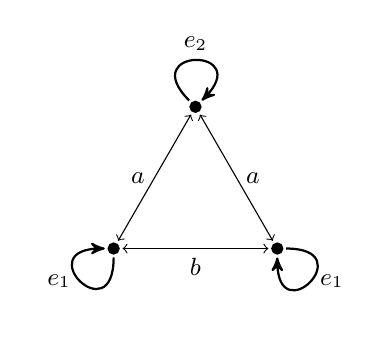
\begin{tikzpicture}[<->,shorten <=1pt,shorten >=1pt,label distance=0mm, font=\small]
\tikzstyle{vertex}=[circle, fill=black, draw=black, inner sep = 0.05cm]

\node[vertex] (1) at (90:1.2cm) {};
\node[vertex] (2) at (210:1.2cm) {};
\node[vertex] (3) at (-30:1.2cm) {};

\draw (1) to node[midway, right] {$a$} (3);
\draw (3) to node[midway, below] {$b$} (2);
\draw (1) to node[midway, left] {$a$} (2);

\Loop[dist=1cm,dir=NO,label=$e_2$,labelstyle=above](1);
\Loop[dist=1cm,dir=SOWE,label=$e_1$,labelstyle=left](2);
\Loop[dist=1cm,dir=SOEA,label=$e_1$,labelstyle=right](3);

\end{tikzpicture}
}      \\[15mm]

$
\begin{array}{|c|cccc|} \hline
\#13 & e_1 & e_2 & a & b \\ \hline
e_1 & e_1 & 0 & a & b \\
e_2 & 0 & e_2 & 0 & b \\
a & a & 0 & e_1 \join b & a \\
b & b & b & a & \id \\ \hline
\end{array}
$
%identity: {'a', 'b'}
%[('c', 'c'), ('b', 'b'), ('d', 'd')]
 & no  
 & no      \\[15mm]

$
\begin{array}{|c|cccc|} \hline
\#14 & e_1 & e_2 & a & b \\ \hline
e_1 & e_1 & 0 & a & b \\
e_2 & 0 & e_2 & a & b \\
a & a & a & -a & a \\
b & b & b & a & \id \\ \hline
\end{array}
$
%identity: {'a', 'b'}
%[('c', 'c'), ('b', 'b'), ('d', 'd')]
 & no  
 & \adjustbox{valign=c, max height=1.7cm}{
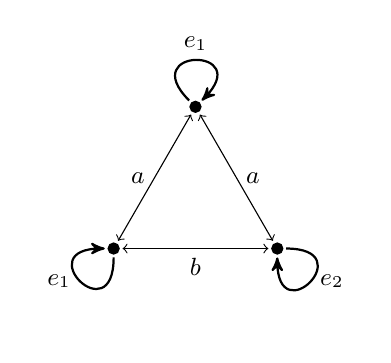
\begin{tikzpicture}[<->,shorten <=1pt,shorten >=1pt,label distance=0mm, font=\small]
\tikzstyle{vertex}=[circle, fill=black, draw=black, inner sep = 0.05cm]

\node[vertex] (1) at (90:1.2cm) {};
\node[vertex] (2) at (210:1.2cm) {};
\node[vertex] (3) at (-30:1.2cm) {};

\draw (1) to node[midway, right] {$a$} (3);
\draw (3) to node[midway, below] {$b$} (2);
\draw (1) to node[midway, left] {$a$} (2);

\Loop[dist=1cm,dir=NO,label=$e_1$,labelstyle=above](1);
\Loop[dist=1cm,dir=SOWE,label=$e_1$,labelstyle=left](2);
\Loop[dist=1cm,dir=SOEA,label=$e_2$,labelstyle=right](3);

\end{tikzpicture}
}      \\[15mm]

$
\begin{array}{|c|cccc|} \hline
\#15 & e_1 & e_2 & a & b \\ \hline
e_1 & e_1 & 0 & a & b \\
e_2 & 0 & e_2 & 0 & 0 \\
a & a & 0 & -e_2 & a \\
b & b & 0 & a & e_1 \\ \hline
\end{array}
$
 & yes
 & \begin{tabular}{c} not simple: \\ $\#2_{\le 3} \times \#14_{\le 3}$ \end{tabular}      \\[15mm]

$
\begin{array}{|c|cccc|} \hline
\#16 & e_1 & e_2 & a & b \\ \hline
e_1 & e_1 & 0 & 0 & b \\
e_2 & 0 & e_2 & a & 0 \\
a & 0 & a & -e_1 & a \\
b & b & 0 & a & e_1 \\ \hline
\end{array}
$
 & no  
 & no      \\[15mm]

$
\begin{array}{|c|cccc|} \hline
\#17 & e_1 & e_2 & a & b \\ \hline
e_1 & e_1 & 0 & a & b \\
e_2 & 0 & e_2 & a & 0 \\
a & a & a & \top & a \\
b & b & 0 & a & e_1 \\ \hline
\end{array}
$
%identity: {'a', 'b'}
%[('c', 'c'), ('b', 'b'), ('d', 'd')]
 & no  
 & \adjustbox{valign=c, max height=1.7cm}{
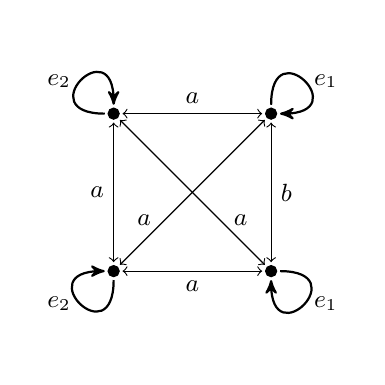
\begin{tikzpicture}[<->,shorten <=1pt,shorten >=1pt,label distance=0mm, font=\small]
\tikzstyle{vertex}=[circle, fill=black, draw=black, inner sep = 0.05cm]

\node[vertex] (1) at (-1,1cm) {};
\node[vertex] (2) at (1,1cm) {};
\node[vertex] (3) at (1,-1cm) {};
\node[vertex] (4) at (-1,-1cm) {};

\draw (1) to node[midway, above] {$a$} (2);
\draw (2) to node[midway, right] {$b$} (3);
\draw (3) to node[midway, below] {$a$} (4);
\draw (1) to node[midway, left] {$a$} (4);
\draw (1) to node[label={[label distance=-1mm, pos=0.75]45:$a$}] {} (3);
\draw (2) to node[label={[label distance=-1mm, pos=0.75]135:$a$}] {} (4);

\Loop[dist=1cm,dir=NOWE,label=$e_2$,labelstyle=left](1);
\Loop[dist=1cm,dir=NOEA,label=$e_1$,labelstyle=right](2);
\Loop[dist=1cm,dir=SOEA,label=$e_1$,labelstyle=right](3);
\Loop[dist=1cm,dir=SOWE,label=$e_2$,labelstyle=left](4);

\end{tikzpicture}
}      \\[15mm]

$
\begin{array}{|c|cccc|} \hline
\#18 & e_1 & e_2 & a & b \\ \hline
e_1 & e_1 & 0 & a & b \\
e_2 & 0 & e_2 & 0 & b \\
a & a & 0 & -e_2 & a \\
b & b & b & a & \id \\ \hline
\end{array}
$
%identity: {'a', 'b'}
%[('c', 'c'), ('b', 'b'), ('d', 'd')]
 & no  
 & no      \\[15mm]

$
\begin{array}{|c|cccc|} \hline
\#19 & e_1 & e_2 & a & b \\ \hline
e_1 & e_1 & 0 & a & b \\
e_2 & 0 & e_2 & a & b \\
a & a & a & \top & a \\
b & b & b & a & \id \\ \hline
\end{array}
$
%identity: {'a', 'b'}
%[('c', 'c'), ('b', 'b'), ('d', 'd')]
 & no  
 & \adjustbox{valign=c, max height=1.7cm}{
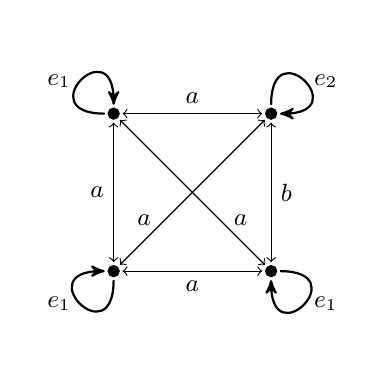
\begin{tikzpicture}[<->,shorten <=1pt,shorten >=1pt,label distance=0mm, font=\small]
\tikzstyle{vertex}=[circle, fill=black, draw=black, inner sep = 0.05cm]

\node[vertex] (1) at (-1,1cm) {};
\node[vertex] (2) at (1,1cm) {};
\node[vertex] (3) at (1,-1cm) {};
\node[vertex] (4) at (-1,-1cm) {};

\draw (1) to node[midway, above] {$a$} (2);
\draw (2) to node[midway, right] {$b$} (3);
\draw (3) to node[midway, below] {$a$} (4);
\draw (1) to node[midway, left] {$a$} (4);
\draw (1) to node[label={[label distance=-1mm, pos=0.75]45:$a$}] {} (3);
\draw (2) to node[label={[label distance=-1mm, pos=0.75]135:$a$}] {} (4);

\Loop[dist=1cm,dir=NOWE,label=$e_1$,labelstyle=left](1);
\Loop[dist=1cm,dir=NOEA,label=$e_2$,labelstyle=right](2);
\Loop[dist=1cm,dir=SOEA,label=$e_1$,labelstyle=right](3);
\Loop[dist=1cm,dir=SOWE,label=$e_1$,labelstyle=left](4);

\end{tikzpicture}
}      \\[15mm]

$
\begin{array}{|c|cccc|} \hline
\#20 & e_1 & e_2 & a & b \\ \hline
e_1 & e_1 & 0 & a & b \\
e_2 & 0 & e_2 & 0 & 0 \\
a & a & 0 & e_1 \join a & b \\
b & b & 0 & b & e_1 \join a \\ \hline
\end{array}
$
%identity: {'a', 'b'}
%[('c', 'c'), ('b', 'b'), ('d', 'd')]
 & yes
 & \begin{tabular}{c} not simple: \\ $\#2_{\le 3} \times \#13_{\le 3}$ \end{tabular}      \\[15mm]

$
\begin{array}{|c|cccc|} \hline
\#21 & e_1 & e_2 & a & b \\ \hline
e_1 & e_1 & 0 & 0 & b \\
e_2 & 0 & e_2 & a & 0 \\
a & 0 & a & e_2 \join a & b \\
b & b & 0 & b & e_1 \join a \\ \hline
\end{array}
$
%identity: {'a', 'b'}
%[('c', 'c'), ('b', 'b'), ('d', 'd')]
 & no  
 & no      \\[15mm]

$
\begin{array}{|c|cccc|} \hline
\#22 & e_1 & e_2 & a & b \\ \hline
e_1 & e_1 & 0 & a & b \\
e_2 & 0 & e_2 & a & 0 \\
a & a & a & -b & b \\
b & b & 0 & b & e_1 \join a \\ \hline
\end{array}
$
%identity: {'a', 'b'}
%[('c', 'c'), ('b', 'b'), ('d', 'd')]
 & no  
 & no      \\[15mm]

$
\begin{array}{|c|cccc|} \hline
\#23 & e_1 & e_2 & a & b \\ \hline
e_1 & e_1 & 0 & a & b \\
e_2 & 0 & e_2 & 0 & b \\
a & a & 0 & e_1 \join a & b \\
b & b & b & b & -b \\ \hline
\end{array}
$
%identity: {'a', 'b'}
%[('c', 'c'), ('b', 'b'), ('d', 'd')]
 & no  
 & \adjustbox{valign=c, max height=1.7cm}{
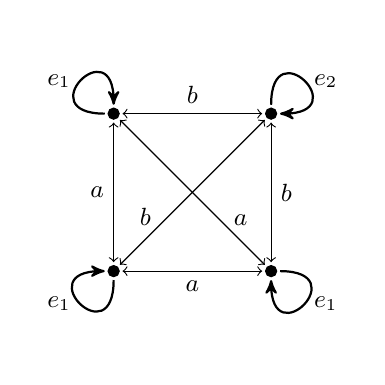
\begin{tikzpicture}[<->,shorten <=1pt,shorten >=1pt,label distance=0mm, font=\small]
\tikzstyle{vertex}=[circle, fill=black, draw=black, inner sep = 0.05cm]

\node[vertex] (1) at (-1,1cm) {};
\node[vertex] (2) at (1,1cm) {};
\node[vertex] (3) at (1,-1cm) {};
\node[vertex] (4) at (-1,-1cm) {};

\draw (1) to node[midway, above] {$b$} (2);
\draw (2) to node[midway, right] {$b$} (3);
\draw (3) to node[midway, below] {$a$} (4);
\draw (1) to node[midway, left] {$a$} (4);
\draw (1) to node[label={[label distance=-1mm, pos=0.75]45:$a$}] {} (3);
\draw (2) to node[label={[label distance=-1mm, pos=0.75]135:$b$}] {} (4);

\Loop[dist=1cm,dir=NOWE,label=$e_1$,labelstyle=left](1);
\Loop[dist=1cm,dir=NOEA,label=$e_2$,labelstyle=right](2);
\Loop[dist=1cm,dir=SOEA,label=$e_1$,labelstyle=right](3);
\Loop[dist=1cm,dir=SOWE,label=$e_1$,labelstyle=left](4);

\end{tikzpicture}
}      \\[15mm]

$
\begin{array}{|c|cccc|} \hline
\#24 & e_1 & e_2 & a & b \\ \hline
e_1 & e_1 & 0 & a & b \\
e_2 & 0 & e_2 & a & b \\
a & a & a & -b & b \\
b & b & b & b & -b \\ \hline
\end{array}
$
%identity: {'a', 'b'}
%[('c', 'c'), ('b', 'b'), ('d', 'd')]
 & no  
 & \adjustbox{valign=c, max height=1.7cm}{
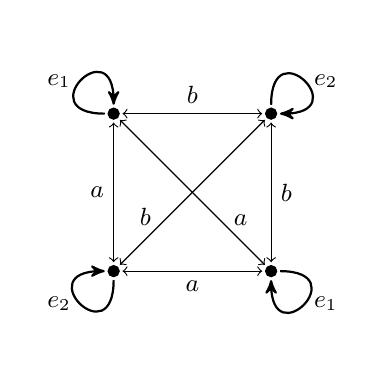
\begin{tikzpicture}[<->,shorten <=1pt,shorten >=1pt,label distance=0mm, font=\small]
\tikzstyle{vertex}=[circle, fill=black, draw=black, inner sep = 0.05cm]

\node[vertex] (1) at (-1,1cm) {};
\node[vertex] (2) at (1,1cm) {};
\node[vertex] (3) at (1,-1cm) {};
\node[vertex] (4) at (-1,-1cm) {};

\draw (1) to node[midway, above] {$b$} (2);
\draw (2) to node[midway, right] {$b$} (3);
\draw (3) to node[midway, below] {$a$} (4);
\draw (1) to node[midway, left] {$a$} (4);
\draw (1) to node[label={[label distance=-1mm, pos=0.75]45:$a$}] {} (3);
\draw (2) to node[label={[label distance=-1mm, pos=0.75]135:$b$}] {} (4);

\Loop[dist=1cm,dir=NOWE,label=$e_1$,labelstyle=left](1);
\Loop[dist=1cm,dir=NOEA,label=$e_2$,labelstyle=right](2);
\Loop[dist=1cm,dir=SOEA,label=$e_1$,labelstyle=right](3);
\Loop[dist=1cm,dir=SOWE,label=$e_2$,labelstyle=left](4);

\end{tikzpicture}
}      \\[15mm]

$
\begin{array}{|c|cccc|} \hline
\#25 & e_1 & e_2 & a & b \\ \hline
e_1 & e_1 & 0 & a & b \\
e_2 & 0 & e_2 & 0 & 0 \\
a & a & 0 & e_1 \join b & a \join b \\
b & b & 0 & a \join b & e_1 \join a \\ \hline
\end{array}
$
%identity: {'a', 'b'}
%[('c', 'c'), ('b', 'b'), ('d', 'd')]
 & yes
 & \begin{tabular}{c} not simple: \\ $\#2_{\le 3} \times \#16_{\le 3}$ \end{tabular}      \\[15mm]

$
\begin{array}{|c|cccc|} \hline
\#26 & e_1 & e_2 & a & b \\ \hline
e_1 & e_1 & 0 & 0 & b \\
e_2 & 0 & e_2 & a & 0 \\
a & 0 & a & e_2 \join b & a \join b \\
b & b & 0 & a \join b & e_1 \join a \\ \hline
\end{array}
$
%identity: {'a', 'b'}
%[('c', 'c'), ('b', 'b'), ('d', 'd')]
 & no  
 & no      \\[15mm]

$
\begin{array}{|c|cccc|} \hline
\#27 & e_1 & e_2 & a & b \\ \hline
e_1 & e_1 & 0 & a & b \\
e_2 & 0 & e_2 & a & 0 \\
a & a & a & -a & a \join b \\
b & b & 0 & a \join b & e_1 \join a \\ \hline
\end{array}
$
%identity: {'a', 'b'}
%[('c', 'c'), ('b', 'b'), ('d', 'd')]
 & no  
 & \adjustbox{valign=c, max height=1.7cm}{
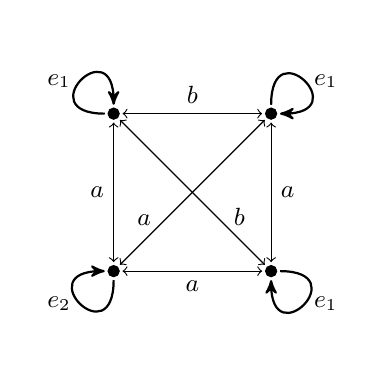
\begin{tikzpicture}[<->,shorten <=1pt,shorten >=1pt,label distance=0mm, font=\small]
\tikzstyle{vertex}=[circle, fill=black, draw=black, inner sep = 0.05cm]

\node[vertex] (1) at (-1,1cm) {};
\node[vertex] (2) at (1,1cm) {};
\node[vertex] (3) at (1,-1cm) {};
\node[vertex] (4) at (-1,-1cm) {};

\draw (1) to node[midway, above] {$b$} (2);
\draw (2) to node[midway, right] {$a$} (3);
\draw (3) to node[midway, below] {$a$} (4);
\draw (1) to node[midway, left] {$a$} (4);
\draw (1) to node[label={[label distance=-1mm, pos=0.75]45:$b$}] {} (3);
\draw (2) to node[label={[label distance=-1mm, pos=0.75]135:$a$}] {} (4);

\Loop[dist=1cm,dir=NOWE,label=$e_1$,labelstyle=left](1);
\Loop[dist=1cm,dir=NOEA,label=$e_1$,labelstyle=right](2);
\Loop[dist=1cm,dir=SOEA,label=$e_1$,labelstyle=right](3);
\Loop[dist=1cm,dir=SOWE,label=$e_2$,labelstyle=left](4);

\end{tikzpicture}
}      \\[15mm]

$
\begin{array}{|c|cccc|} \hline
\#28 & e_1 & e_2 & a & b \\ \hline
e_1 & e_1 & 0 & a & b \\
e_2 & 0 & e_2 & a & b \\
a & a & a & -a & a \join b \\
b & b & b & a \join b & -b \\ \hline
\end{array}
$
%identity: {'a', 'b'}
%[('c', 'c'), ('b', 'b'), ('d', 'd')]
 & no  
 & \adjustbox{valign=c, max height=1.7cm}{
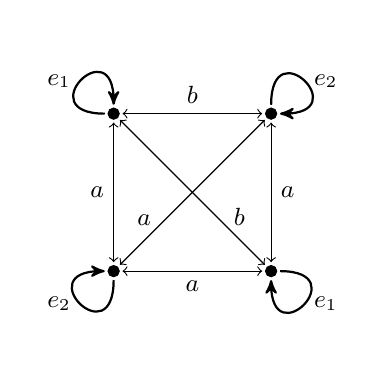
\begin{tikzpicture}[<->,shorten <=1pt,shorten >=1pt,label distance=0mm, font=\small]
\tikzstyle{vertex}=[circle, fill=black, draw=black, inner sep = 0.05cm]

\node[vertex] (1) at (-1,1cm) {};
\node[vertex] (2) at (1,1cm) {};
\node[vertex] (3) at (1,-1cm) {};
\node[vertex] (4) at (-1,-1cm) {};

\draw (1) to node[midway, above] {$b$} (2);
\draw (2) to node[midway, right] {$a$} (3);
\draw (3) to node[midway, below] {$a$} (4);
\draw (1) to node[midway, left] {$a$} (4);
\draw (1) to node[label={[label distance=-1mm, pos=0.75]45:$b$}] {} (3);
\draw (2) to node[label={[label distance=-1mm, pos=0.75]135:$a$}] {} (4);

\Loop[dist=1cm,dir=NOWE,label=$e_1$,labelstyle=left](1);
\Loop[dist=1cm,dir=NOEA,label=$e_2$,labelstyle=right](2);
\Loop[dist=1cm,dir=SOEA,label=$e_1$,labelstyle=right](3);
\Loop[dist=1cm,dir=SOWE,label=$e_2$,labelstyle=left](4);

\end{tikzpicture}
}     \\[15mm]

$
\begin{array}{|c|cccc|} \hline
\#29 & e_1 & e_2 & a & b \\ \hline
e_1 & e_1 & 0 & a & b \\
e_2 & 0 & e_2 & 0 & 0 \\
a & a & 0 & -e_2 & a \join b \\
b & b & 0 & a \join b & e_1 \join a \\ \hline
\end{array}
$
%identity: {'a', 'b'}
%[('c', 'c'), ('b', 'b'), ('d', 'd')]
 & yes
 & \begin{tabular}{c} not simple: \\ $\#2_{\le 3} \times \#17_{\le 3}$ \end{tabular}      \\[15mm]

$
\begin{array}{|c|cccc|} \hline
\#30 & e_1 & e_2 & a & b \\ \hline
e_1 & e_1 & 0 & 0 & b \\
e_2 & 0 & e_2 & a & 0 \\
a & 0 & a & -e_1 & a \join b \\
b & b & 0 & a \join b & e_1 \join a \\ \hline
\end{array}
$
%identity: {'a', 'b'}
%[('c', 'c'), ('b', 'b'), ('d', 'd')]
 & no  
 & no      \\[15mm]

$
\begin{array}{|c|cccc|} \hline
\#31 & e_1 & e_2 & a & b \\ \hline
e_1 & e_1 & 0 & a & b \\
e_2 & 0 & e_2 & a & 0 \\
a & a & a & \top & a \join b \\
b & b & 0 & a \join b & e_1 \join a \\ \hline
\end{array}
$
%identity: {'a', 'b'}
%[('c', 'c'), ('b', 'b'), ('d', 'd')]
 & no  
 & \adjustbox{valign=c, max height=1.7cm}{
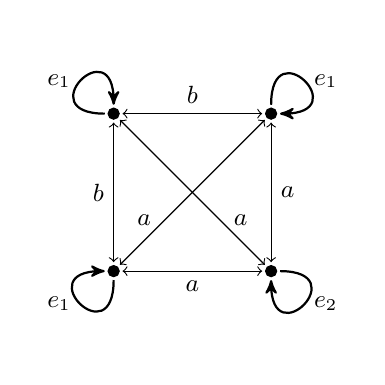
\begin{tikzpicture}[<->,shorten <=1pt,shorten >=1pt,label distance=0mm, font=\small]
\tikzstyle{vertex}=[circle, fill=black, draw=black, inner sep = 0.05cm]

\node[vertex] (1) at (-1,1cm) {};
\node[vertex] (2) at (1,1cm) {};
\node[vertex] (3) at (1,-1cm) {};
\node[vertex] (4) at (-1,-1cm) {};

\draw (1) to node[midway, above] {$b$} (2);
\draw (2) to node[midway, right] {$a$} (3);
\draw (3) to node[midway, below] {$a$} (4);
\draw (1) to node[midway, left] {$b$} (4);
\draw (1) to node[label={[label distance=-1mm, pos=0.75]45:$a$}] {} (3);
\draw (2) to node[label={[label distance=-1mm, pos=0.75]135:$a$}] {} (4);

\Loop[dist=1cm,dir=NOWE,label=$e_1$,labelstyle=left](1);
\Loop[dist=1cm,dir=NOEA,label=$e_1$,labelstyle=right](2);
\Loop[dist=1cm,dir=SOEA,label=$e_2$,labelstyle=right](3);
\Loop[dist=1cm,dir=SOWE,label=$e_1$,labelstyle=left](4);

\end{tikzpicture}
}       \\[15mm]

$
\begin{array}{|c|cccc|} \hline
\#32 & e_1 & e_2 & a & b \\ \hline
e_1 & e_1 & 0 & a & b \\
e_2 & 0 & e_2 & 0 & b \\
a & a & 0 & -e_2 & a \join b \\
b & b & b & a \join b & -b \\ \hline
\end{array}
$
%identity: {'a', 'b'}
%[('c', 'c'), ('b', 'b'), ('d', 'd')]
 & no  
 & no      \\[15mm]

$
\begin{array}{|c|cccc|} \hline
\#33 & e_1 & e_2 & a & b \\ \hline
e_1 & e_1 & 0 & a & b \\
e_2 & 0 & e_2 & a & b \\
a & a & a & \top & a \join b \\
b & b & b & a \join b & -b \\ \hline
\end{array}
$
%identity: {'a', 'b'}
%[('c', 'c'), ('b', 'b'), ('d', 'd')]
 & no  
 & \adjustbox{valign=c, max height=1.7cm}{
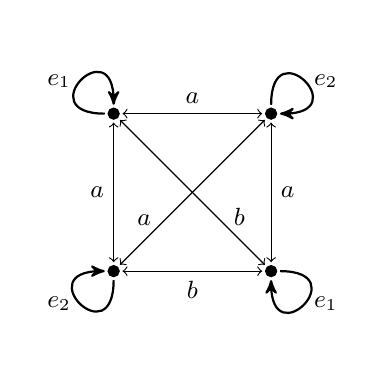
\begin{tikzpicture}[<->,shorten <=1pt,shorten >=1pt,label distance=0mm, font=\small]
\tikzstyle{vertex}=[circle, fill=black, draw=black, inner sep = 0.05cm]

\node[vertex] (1) at (-1,1cm) {};
\node[vertex] (2) at (1,1cm) {};
\node[vertex] (3) at (1,-1cm) {};
\node[vertex] (4) at (-1,-1cm) {};

\draw (1) to node[midway, above] {$a$} (2);
\draw (2) to node[midway, right] {$a$} (3);
\draw (3) to node[midway, below] {$b$} (4);
\draw (1) to node[midway, left] {$a$} (4);
\draw (1) to node[label={[label distance=-1mm, pos=0.75]45:$b$}] {} (3);
\draw (2) to node[label={[label distance=-1mm, pos=0.75]135:$a$}] {} (4);

\Loop[dist=1cm,dir=NOWE,label=$e_1$,labelstyle=left](1);
\Loop[dist=1cm,dir=NOEA,label=$e_2$,labelstyle=right](2);
\Loop[dist=1cm,dir=SOEA,label=$e_1$,labelstyle=right](3);
\Loop[dist=1cm,dir=SOWE,label=$e_2$,labelstyle=left](4);

\end{tikzpicture}
}      \\[15mm]

$
\begin{array}{|c|cccc|} \hline
\#34 & e_1 & e_2 & a & b \\ \hline
e_1 & e_1 & 0 & a & b \\
e_2 & 0 & e_2 & 0 & 0 \\
a & a & 0 & e_1 \join a & 0 \\
b & b & 0 & 0 & e_1 \join b \\ \hline
\end{array}
$
%identity: {'a', 'b'}
%[('c', 'c'), ('b', 'b'), ('d', 'd')]
 & no  
 & \begin{tabular}{c} not simple: \\ $\#2_{\le 3} \times \#24_{\le 3}$ \end{tabular}      \\[15mm]

$
\begin{array}{|c|cccc|} \hline
\#35 & e_1 & e_2 & a & b \\ \hline
e_1 & e_1 & 0 & 0 & b \\
e_2 & 0 & e_2 & a & 0 \\
a & 0 & a & e_2 \join a & 0 \\
b & b & 0 & 0 & e_1 \join b \\ \hline
\end{array}
$
%identity: {'a', 'b'}
%[('c', 'c'), ('b', 'b'), ('d', 'd')]
 & yes
 & \begin{tabular}{c} not simple: \\ $\#5_{\le 3} \times \#5_{\le 3}$ \end{tabular}      \\[15mm]

$
\begin{array}{|c|cccc|} \hline
\#36 & e_1 & e_2 & a & b \\ \hline
e_1 & e_1 & 0 & a & b \\
e_2 & 0 & e_2 & a & 0 \\
a & a & a & -b & 0 \\
b & b & 0 & 0 & e_1 \join b \\ \hline
\end{array}
$
%identity: {'a', 'b'}
%[('c', 'c'), ('b', 'b'), ('d', 'd')]
 & no  
 & no      \\[15mm]

$
\begin{array}{|c|cccc|} \hline
\#37 & e_1 & e_2 & a & b \\ \hline
e_1 & e_1 & 0 & a & b \\
e_2 & 0 & e_2 & a & b \\
a & a & a & -b & 0 \\
b & b & b & 0 & -a \\ \hline
\end{array}
$
%identity: {'a', 'b'}
%[('c', 'c'), ('b', 'b'), ('d', 'd')]
 & no  
 & no      \\[15mm]

$
\begin{array}{|c|cccc|} \hline
\#38 & e_1 & e_2 & a & b \\ \hline
e_1 & e_1 & 0 & a & b \\
e_2 & 0 & e_2 & 0 & 0 \\
a & a & 0 & -e_2 & a \\
b & b & 0 & a & e_1 \join b \\ \hline
\end{array}
$
%identity: {'a', 'b'}
%[('c', 'c'), ('b', 'b'), ('d', 'd')]
 & yes
 & \begin{tabular}{c} not simple: \\ $\#2_{\le 3} \times \#15_{\le 3}$ \end{tabular}      \\[15mm]

$
\begin{array}{|c|cccc|} \hline
\#39 & e_1 & e_2 & a & b \\ \hline
e_1 & e_1 & 0 & 0 & b \\
e_2 & 0 & e_2 & a & 0 \\
a & 0 & a & -e_1 & a \\
b & b & 0 & a & e_1 \join b \\ \hline
\end{array}
$
%identity: {'a', 'b'}
%[('c', 'c'), ('b', 'b'), ('d', 'd')]
 & no  
 & no      \\[15mm]

$
\begin{array}{|c|cccc|} \hline
\#40 & e_1 & e_2 & a & b \\ \hline
e_1 & e_1 & 0 & a & b \\
e_2 & 0 & e_2 & a & 0 \\
a & a & a & \top & a \\
b & b & 0 & a & e_1 \join b \\ \hline
\end{array}
$
 & no  
 & \adjustbox{valign=c, max height=1.7cm}{
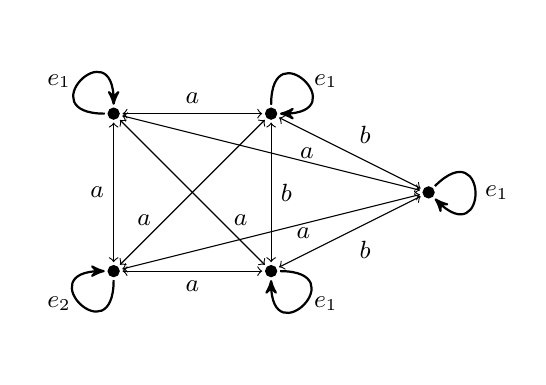
\begin{tikzpicture}[<->,shorten <=1pt,shorten >=1pt,label distance=0mm, font=\small]
\tikzstyle{vertex}=[circle, fill=black, draw=black, inner sep = 0.05cm]

\node[vertex] (1) at (-1,1cm) {};
\node[vertex] (2) at (1,1cm) {};
\node[vertex] (3) at (1,-1cm) {};
\node[vertex] (4) at (-1,-1cm) {};
\node[vertex] (5) at (3,0cm) {};

\draw (1) to node[midway, above] {$a$} (2);
\draw (2) to node[midway, right] {$b$} (3);
\draw (3) to node[midway, below] {$a$} (4);
\draw (1) to node[midway, left] {$a$} (4);
\draw (1) to node[label={[label distance=-1mm, pos=0.75]45:$a$}] {} (3);
\draw (2) to node[label={[label distance=-1mm, pos=0.75]135:$a$}] {} (4);
\draw (5) to node[midway, above right] {$b$} (2);
\draw (5) to node[label={[label distance=-1mm, pos=0.35]150:$a$}] {} (1);
\draw (5) to node[label={[label distance=-0.5mm, pos=0.35]-150:$a$}] {} (4);
\draw (5) to node[midway, below right] {$b$} (3);

\Loop[dist=1cm,dir=NOWE,label=$e_1$,labelstyle=left](1);
\Loop[dist=1cm,dir=NOEA,label=$e_1$,labelstyle=right](2);
\Loop[dist=1cm,dir=SOEA,label=$e_1$,labelstyle=right](3);
\Loop[dist=1cm,dir=SOWE,label=$e_2$,labelstyle=left](4);
\Loop[dist=1cm,dir=EA,label=$e_1$,labelstyle=right](5);

\end{tikzpicture}
}       \\[15mm]

$
\begin{array}{|c|cccc|} \hline
\#41 & e_1 & e_2 & a & b \\ \hline
e_1 & e_1 & 0 & a & b \\
e_2 & 0 & e_2 & 0 & b \\
a & a & 0 & -e_2 & a \\
b & b & b & a & -a \\ \hline
\end{array}
$
 & no  
 & no      \\[15mm]

$
\begin{array}{|c|cccc|} \hline
\#42 & e_1 & e_2 & a & b \\ \hline
e_1 & e_1 & 0 & a & b \\
e_2 & 0 & e_2 & a & b \\
a & a & a & \top & a \\
b & b & b & a & -a \\ \hline
\end{array}
$
 & no  
 & \adjustbox{valign=c, max height=1.7cm}{
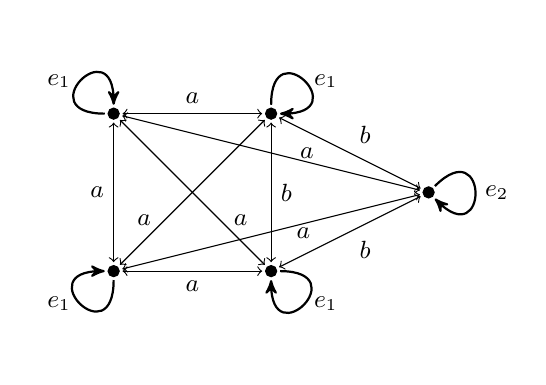
\begin{tikzpicture}[<->,shorten <=1pt,shorten >=1pt,label distance=0mm, font=\small]
\tikzstyle{vertex}=[circle, fill=black, draw=black, inner sep = 0.05cm]

\node[vertex] (1) at (-1,1cm) {};
\node[vertex] (2) at (1,1cm) {};
\node[vertex] (3) at (1,-1cm) {};
\node[vertex] (4) at (-1,-1cm) {};
\node[vertex] (5) at (3,0cm) {};

\draw (1) to node[midway, above] {$a$} (2);
\draw (2) to node[midway, right] {$b$} (3);
\draw (3) to node[midway, below] {$a$} (4);
\draw (1) to node[midway, left] {$a$} (4);
\draw (1) to node[label={[label distance=-1mm, pos=0.75]45:$a$}] {} (3);
\draw (2) to node[label={[label distance=-1mm, pos=0.75]135:$a$}] {} (4);
\draw (5) to node[midway, above right] {$b$} (2);
\draw (5) to node[label={[label distance=-1mm, pos=0.35]150:$a$}] {} (1);
\draw (5) to node[label={[label distance=-0.5mm, pos=0.35]-150:$a$}] {} (4);
\draw (5) to node[midway, below right] {$b$} (3);

\Loop[dist=1cm,dir=NOWE,label=$e_1$,labelstyle=left](1);
\Loop[dist=1cm,dir=NOEA,label=$e_1$,labelstyle=right](2);
\Loop[dist=1cm,dir=SOEA,label=$e_1$,labelstyle=right](3);
\Loop[dist=1cm,dir=SOWE,label=$e_1$,labelstyle=left](4);
\Loop[dist=1cm,dir=EA,label=$e_2$,labelstyle=right](5);

\end{tikzpicture}
}      \\[15mm]

$
\begin{array}{|c|cccc|} \hline
\#43 & e_1 & e_2 & a & b \\ \hline
e_1 & e_1 & 0 & a & b \\
e_2 & 0 & e_2 & 0 & 0 \\
a & a & 0 & -e_2 & a \join b \\
b & b & 0 & a \join b & -e_2 \\ \hline
\end{array}
$
 & yes
 & \begin{tabular}{c} not simple: \\ $\#2_{\le 3} \times \#18_{\le 3}$ \end{tabular}      \\[15mm]

$
\begin{array}{|c|cccc|} \hline
\#44 & e_1 & e_2 & a & b \\ \hline
e_1 & e_1 & 0 & 0 & b \\
e_2 & 0 & e_2 & a & 0 \\
a & 0 & a & -e_1 & a \join b \\
b & b & 0 & a \join b & -e_2 \\ \hline
\end{array}
$
 & no  
 & no      \\[15mm]

$
\begin{array}{|c|cccc|} \hline
\#45 & e_1 & e_2 & a & b \\ \hline
e_1 & e_1 & 0 & a & b \\
e_2 & 0 & e_2 & a & 0 \\
a & a & a & \top & a \join b \\
b & b & 0 & a \join b & -e_2 \\ \hline
\end{array}
$
 & no  
 & \adjustbox{valign=c, max height=1.7cm}{
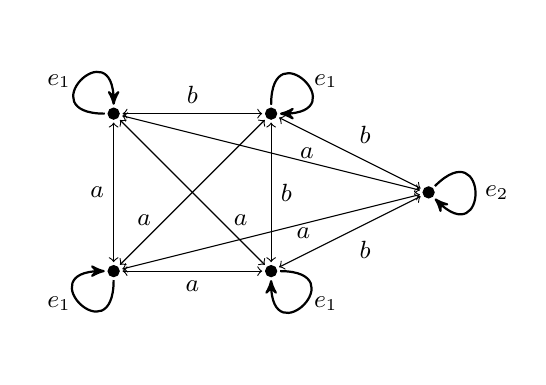
\begin{tikzpicture}[<->,shorten <=1pt,shorten >=1pt,label distance=0mm, font=\small]
\tikzstyle{vertex}=[circle, fill=black, draw=black, inner sep = 0.05cm]

\node[vertex] (1) at (-1,1cm) {};
\node[vertex] (2) at (1,1cm) {};
\node[vertex] (3) at (1,-1cm) {};
\node[vertex] (4) at (-1,-1cm) {};
\node[vertex] (5) at (3,0cm) {};

\draw (1) to node[midway, above] {$b$} (2);
\draw (2) to node[midway, right] {$b$} (3);
\draw (3) to node[midway, below] {$a$} (4);
\draw (1) to node[midway, left] {$a$} (4);
\draw (1) to node[label={[label distance=-1mm, pos=0.75]45:$a$}] {} (3);
\draw (2) to node[label={[label distance=-1mm, pos=0.75]135:$a$}] {} (4);
\draw (5) to node[midway, above right] {$b$} (2);
\draw (5) to node[label={[label distance=-1mm, pos=0.35]150:$a$}] {} (1);
\draw (5) to node[label={[label distance=-0.5mm, pos=0.35]-150:$a$}] {} (4);
\draw (5) to node[midway, below right] {$b$} (3);

\Loop[dist=1cm,dir=NOWE,label=$e_1$,labelstyle=left](1);
\Loop[dist=1cm,dir=NOEA,label=$e_1$,labelstyle=right](2);
\Loop[dist=1cm,dir=SOEA,label=$e_1$,labelstyle=right](3);
\Loop[dist=1cm,dir=SOWE,label=$e_1$,labelstyle=left](4);
\Loop[dist=1cm,dir=EA,label=$e_2$,labelstyle=right](5);

\end{tikzpicture}
}      \\[15mm]

$
\begin{array}{|c|cccc|} \hline
\#46 & e_1 & e_2 & a & b \\ \hline
e_1 & e_1 & 0 & a & b \\
e_2 & 0 & e_2 & a & b \\
a & a & a & \top & a \join b \\
b & b & b & a \join b & \top \\ \hline
\end{array}
$
 & no  
 & \adjustbox{valign=c, max height=1.7cm}{
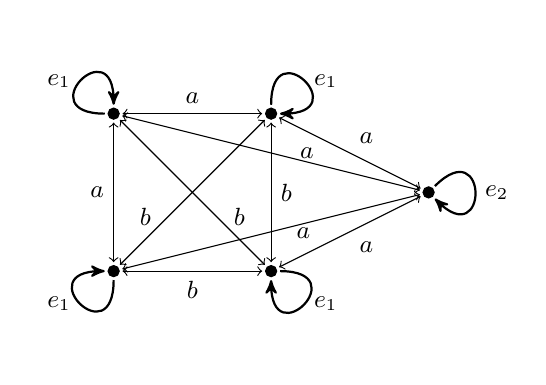
\begin{tikzpicture}[<->,shorten <=1pt,shorten >=1pt,label distance=0mm, font=\small]
\tikzstyle{vertex}=[circle, fill=black, draw=black, inner sep = 0.05cm]

\node[vertex] (1) at (-1,1cm) {};
\node[vertex] (2) at (1,1cm) {};
\node[vertex] (3) at (1,-1cm) {};
\node[vertex] (4) at (-1,-1cm) {};
\node[vertex] (5) at (3,0cm) {};

\draw (1) to node[midway, above] {$a$} (2);
\draw (2) to node[midway, right] {$b$} (3);
\draw (3) to node[midway, below] {$b$} (4);
\draw (1) to node[midway, left] {$a$} (4);
\draw (1) to node[label={[label distance=-1mm, pos=0.75]45:$b$}] {} (3);
\draw (2) to node[label={[label distance=-1mm, pos=0.75]135:$b$}] {} (4);
\draw (5) to node[midway, above right] {$a$} (2);
\draw (5) to node[label={[label distance=-1mm, pos=0.35]150:$a$}] {} (1);
\draw (5) to node[label={[label distance=-0.5mm, pos=0.35]-150:$a$}] {} (4);
\draw (5) to node[midway, below right] {$a$} (3);

\Loop[dist=1cm,dir=NOWE,label=$e_1$,labelstyle=left](1);
\Loop[dist=1cm,dir=NOEA,label=$e_1$,labelstyle=right](2);
\Loop[dist=1cm,dir=SOEA,label=$e_1$,labelstyle=right](3);
\Loop[dist=1cm,dir=SOWE,label=$e_1$,labelstyle=left](4);
\Loop[dist=1cm,dir=EA,label=$e_2$,labelstyle=right](5);

\end{tikzpicture}
}      \\[15mm]

\end{longtable}
\end{center}

\section[Two fragment identity and one nonsymmetric]{Atoms: two fragment identity and one nonsymmetric}

\begin{center}
\begin{longtable}{l|c|c}
  atom table & RA  & QRNA \\ \hline && \\[-4mm]  \endhead 
  \hline \endfoot

$
\begin{array}{|c|cccc|} \hline
\#47 & e_1 & e_2 & r & \con{r} \\ \hline
e_1 & e_1 & 0 & r & \con{r} \\
e_2 & 0 & e_2 & 0 & 0 \\
r & r & 0 & 0 & e_1 \\
\con{r} & \con{r} & 0 & e_1 & 0 \\ \hline
\end{array}
$
 & no  
 & \begin{tabular}{c} not simple: \\ $\#2_{\le 3} \times \#21_{\le 3}$ \end{tabular}      \\[15mm]

$
\begin{array}{|c|cccc|} \hline
\#48 & e_1 & e_2 & r & \con{r} \\ \hline
e_1 & e_1 & 0 & 0 & \con{r} \\
e_2 & 0 & e_2 & r & 0 \\
r & r & 0 & 0 & e_2 \\
\con{r} & 0 & \con{r} & e_1 & 0 \\ \hline
\end{array}
$
 & yes
 & \adjustbox{valign=c, max height=1.7cm}{
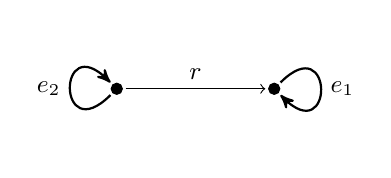
\begin{tikzpicture}[->,shorten <=1pt,shorten >=1pt,label distance=0mm, font=\small]
\tikzstyle{vertex}=[circle, fill=black, draw=black, inner sep = 0.05cm]

\node[vertex] (1) at (-1,1cm) {};
\node[vertex] (2) at (1,1cm) {};

\draw (1) to node[midway, above] {$r$} (2);

\Loop[dist=1cm,dir=WE,label=$e_2$,labelstyle=left](1);
\Loop[dist=1cm,dir=EA,label=$e_1$,labelstyle=right](2);

\end{tikzpicture}
}      \\[15mm]

$
\begin{array}{|c|cccc|} \hline
\#49 & e_1 & e_2 & r & \con{r} \\ \hline
e_1 & e_1 & 0 & r & \con{r} \\
e_2 & 0 & e_2 & r & 0 \\
r & r & 0 & 0 & \id \\
\con{r} & \con{r} & \con{r} & e_1 & 0 \\ \hline
\end{array}
$
 & no  
 & no      \\[15mm]

$
\begin{array}{|c|cccc|} \hline
\#50 & e_1 & e_2 & r & \con{r} \\ \hline
e_1 & e_1 & 0 & r & \con{r} \\
e_2 & 0 & e_2 & r & \con{r} \\
r & r & r & 0 & \id \\
\con{r} & \con{r} & \con{r} & \id & 0 \\ \hline
\end{array}
$
 & no  
 & no      \\[15mm]

$
\begin{array}{|c|cccc|} \hline
\#51 & e_1 & e_2 & r & \con{r} \\ \hline
e_1 & e_1 & 0 & r & \con{r} \\
e_2 & 0 & e_2 & 0 & 0 \\
r & r & 0 & r & -e_2 \\
\con{r} & \con{r} & 0 & -e_2 & \con{r} \\ \hline
\end{array}
$
 & yes
 & \begin{tabular}{c} not simple: \\ $\#2_{\le 3} \times \#10_{\le 3}$ \end{tabular}       \\[15mm]

$
\begin{array}{|c|cccc|} \hline
\#52 & e_1 & e_2 & r & \con{r} \\ \hline
e_1 & e_1 & 0 & 0 & \con{r} \\
e_2 & 0 & e_2 & r & 0 \\
r & r & 0 & r & -e_1 \\
\con{r} & 0 & \con{r} & -e_2 & \con{r} \\ \hline
\end{array}
$
 & no  
 & no      \\[15mm]

$
\begin{array}{|c|cccc|} \hline
\#53 & e_1 & e_2 & r & \con{r} \\ \hline
e_1 & e_1 & 0 & r & \con{r} \\
e_2 & 0 & e_2 & r & 0 \\
r & r & 0 & r & \top \\
\con{r} & \con{r} & \con{r} & -e_2 & \con{r} \\ \hline
\end{array}
$
 & no  
 & \adjustbox{valign=c, max height=1.7cm}{
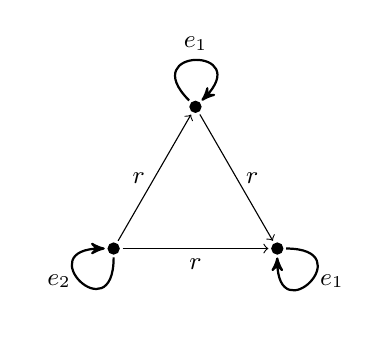
\begin{tikzpicture}[->,shorten <=1pt,shorten >=1pt,label distance=0mm, font=\small]
\tikzstyle{vertex}=[circle, fill=black, draw=black, inner sep = 0.05cm]

\node[vertex] (1) at (90:1.2cm) {};
\node[vertex] (2) at (210:1.2cm) {};
\node[vertex] (3) at (-30:1.2cm) {};

\draw (1) to node[midway, right] {$r$} (3);
\draw (2) to node[midway, below] {$r$} (3);
\draw (2) to node[midway, left] {$r$} (1);

\Loop[dist=1cm,dir=NO,label=$e_1$,labelstyle=above](1);
\Loop[dist=1cm,dir=SOWE,label=$e_2$,labelstyle=left](2);
\Loop[dist=1cm,dir=SOEA,label=$e_1$,labelstyle=right](3);

\end{tikzpicture}
}      \\[15mm]

$
\begin{array}{|c|cccc|} \hline
\#54 & e_1 & e_2 & r & \con{r} \\ \hline
e_1 & e_1 & 0 & r & \con{r} \\
e_2 & 0 & e_2 & r & \con{r} \\
r & r & r & r & \top \\
\con{r} & \con{r} & \con{r} & \top & \con{r} \\ \hline
\end{array}
$
 & no  
 & \adjustbox{valign=c, max height=1.7cm}{
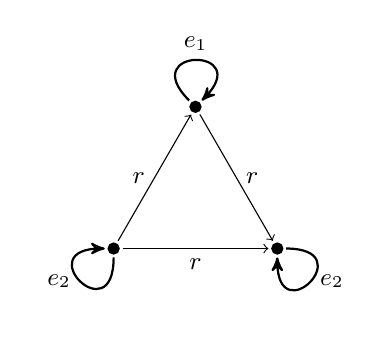
\begin{tikzpicture}[->,shorten <=1pt,shorten >=1pt,label distance=0mm, font=\small]
\tikzstyle{vertex}=[circle, fill=black, draw=black, inner sep = 0.05cm]

\node[vertex] (1) at (90:1.2cm) {};
\node[vertex] (2) at (210:1.2cm) {};
\node[vertex] (3) at (-30:1.2cm) {};

\draw (1) to node[midway, right] {$r$} (3);
\draw (2) to node[midway, below] {$r$} (3);
\draw (2) to node[midway, left] {$r$} (1);

\Loop[dist=1cm,dir=NO,label=$e_1$,labelstyle=above](1);
\Loop[dist=1cm,dir=SOWE,label=$e_2$,labelstyle=left](2);
\Loop[dist=1cm,dir=SOEA,label=$e_2$,labelstyle=right](3);

\end{tikzpicture}
}      \\[15mm]

$
\begin{array}{|c|cccc|} \hline
\#55 & e_1 & e_2 & r & \con{r} \\ \hline
e_1 & e_1 & 0 & r & \con{r} \\
e_2 & 0 & e_2 & 0 & 0 \\
r & r & 0 & \con{r} & e_1 \\
\con{r} & \con{r} & 0 & e_1 & r \\ \hline
\end{array}
$
%identity: {'a', 'b'}
%[('c', 'd'), ('b', 'b')]
 & yes
 & \begin{tabular}{c} not simple: \\ $\#2_{\le 3} \times \#9_{\le 3}$ \end{tabular}      \\[15mm]

$
\begin{array}{|c|cccc|} \hline
\#56 & e_1 & e_2 & r & \con{r} \\ \hline
e_1 & e_1 & 0 & 0 & \con{r} \\
e_2 & 0 & e_2 & r & 0 \\
r & r & 0 & \con{r} & e_2 \\
\con{r} & 0 & \con{r} & e_1 & r \\ \hline
\end{array}
$
%identity: {'a', 'b'}
%[('c', 'd'), ('b', 'b')]
 & no  
 & no      \\[15mm]

$
\begin{array}{|c|cccc|} \hline
\#57 & e_1 & e_2 & r & \con{r} \\ \hline
e_1 & e_1 & 0 & r & \con{r} \\
e_2 & 0 & e_2 & r & 0 \\
r & r & 0 & \con{r} & \id \\
\con{r} & \con{r} & \con{r} & e_1 & r \\ \hline
\end{array}
$
%identity: {'a', 'b'}
%[('c', 'd'), ('b', 'b')]
 & no  
 & no      \\[15mm]

$
\begin{array}{|c|cccc|} \hline
\#58 & e_1 & e_2 & r & \con{r} \\ \hline
e_1 & e_1 & 0 & r & \con{r} \\
e_2 & 0 & e_2 & r & \con{r} \\
r & r & r & \con{r} & \id \\
\con{r} & \con{r} & \con{r} & \id & r \\ \hline
\end{array}
$
%identity: {'a', 'b'}
%[('c', 'd'), ('b', 'b')]
 & no  
 & \adjustbox{valign=c, max height=1.7cm}{
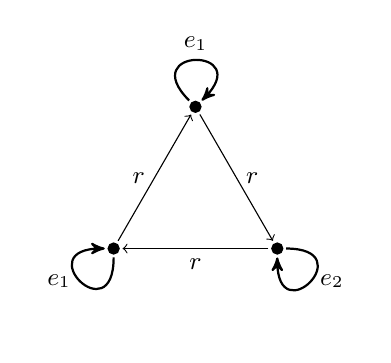
\begin{tikzpicture}[->,shorten <=1pt,shorten >=1pt,label distance=0mm, font=\small]
\tikzstyle{vertex}=[circle, fill=black, draw=black, inner sep = 0.05cm]

\node[vertex] (1) at (90:1.2cm) {};
\node[vertex] (2) at (210:1.2cm) {};
\node[vertex] (3) at (-30:1.2cm) {};

\draw (1) to node[midway, right] {$r$} (3);
\draw (3) to node[midway, below] {$r$} (2);
\draw (2) to node[midway, left] {$r$} (1);

\Loop[dist=1cm,dir=NO,label=$e_1$,labelstyle=above](1);
\Loop[dist=1cm,dir=SOWE,label=$e_1$,labelstyle=left](2);
\Loop[dist=1cm,dir=SOEA,label=$e_2$,labelstyle=right](3);

\end{tikzpicture}
}      \\[15mm]

$
\begin{array}{|c|cccc|} \hline
\#59 & e_1 & e_2 & r & \con{r} \\ \hline
e_1 & e_1 & 0 & r & \con{r} \\
e_2 & 0 & e_2 & 0 & 0 \\
r & r & 0 & r \join \con{r} & -e_2 \\
\con{r} & \con{r} & 0 & -e_2 & r \join \con{r} \\ \hline
\end{array}
$
%identity: {'a', 'b'}
%[('c', 'd'), ('b', 'b')]
 & yes
 & \begin{tabular}{c} not simple: \\ $\#2_{\le 3} \times \#11_{\le 3}$ \end{tabular}      \\[15mm]

$
\begin{array}{|c|cccc|} \hline
\#60 & e_1 & e_2 & r & \con{r} \\ \hline
e_1 & e_1 & 0 & 0 & \con{r} \\
e_2 & 0 & e_2 & r & 0 \\
r & r & 0 & r \join \con{r} & -e_1 \\
\con{r} & 0 & \con{r} & -e_2 & r \join \con{r} \\ \hline
\end{array}
$
%identity: {'a', 'b'}
%[('c', 'd'), ('b', 'b')]
 & no  
 & no      \\[15mm]

$
\begin{array}{|c|cccc|} \hline
\#61 & e_1 & e_2 & r & \con{r} \\ \hline
e_1 & e_1 & 0 & r & \con{r} \\
e_2 & 0 & e_2 & r & 0 \\
r & r & 0 & r \join \con{r} & \top \\
\con{r} & \con{r} & \con{r} & -e_2 & r \join \con{r} \\ \hline
\end{array}
$
%identity: {'a', 'b'}
%[('c', 'd'), ('b', 'b')]
 & no  
 & \adjustbox{valign=c, max height=1.7cm}{
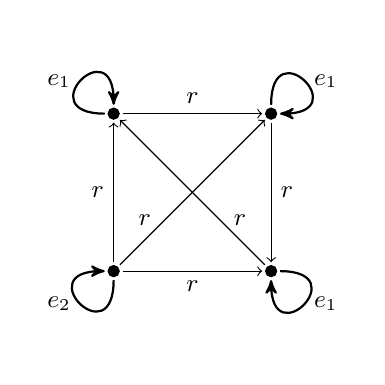
\begin{tikzpicture}[->,shorten <=1pt,shorten >=1pt,label distance=0mm, font=\small]
\tikzstyle{vertex}=[circle, fill=black, draw=black, inner sep = 0.05cm]

\node[vertex] (1) at (-1,1cm) {};
\node[vertex] (2) at (1,1cm) {};
\node[vertex] (3) at (1,-1cm) {};
\node[vertex] (4) at (-1,-1cm) {};

\draw (1) to node[midway, above] {$r$} (2);
\draw (2) to node[midway, right] {$r$} (3);
\draw (4) to node[midway, below] {$r$} (3);
\draw (4) to node[midway, left] {$r$} (1);
\draw (3) to node[label={[label distance=-1mm, pos=0.25]45:$r$}] {} (1);
\draw (4) to node[label={[label distance=-1mm, pos=0.25]135:$r$}] {} (2);

\Loop[dist=1cm,dir=NOWE,label=$e_1$,labelstyle=left](1);
\Loop[dist=1cm,dir=NOEA,label=$e_1$,labelstyle=right](2);
\Loop[dist=1cm,dir=SOEA,label=$e_1$,labelstyle=right](3);
\Loop[dist=1cm,dir=SOWE,label=$e_2$,labelstyle=left](4);

\end{tikzpicture}
}      \\[15mm]

$
\begin{array}{|c|cccc|} \hline
\#62 & e_1 & e_2 & r & \con{r} \\ \hline
e_1 & e_1 & 0 & r & \con{r} \\
e_2 & 0 & e_2 & r & \con{r} \\
r & r & r & r \join \con{r} & \top \\
\con{r} & \con{r} & \con{r} & \top & r \join \con{r} \\ \hline
\end{array}
$
%identity: {'a', 'b'}
%[('c', 'd'), ('b', 'b')]
 & no  
 & \adjustbox{valign=c, max height=1.7cm}{
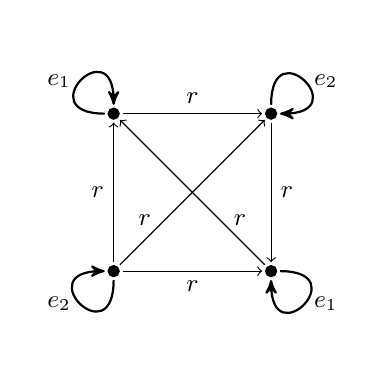
\begin{tikzpicture}[->,shorten <=1pt,shorten >=1pt,label distance=0mm, font=\small]
\tikzstyle{vertex}=[circle, fill=black, draw=black, inner sep = 0.05cm]

\node[vertex] (1) at (-1,1cm) {};
\node[vertex] (2) at (1,1cm) {};
\node[vertex] (3) at (1,-1cm) {};
\node[vertex] (4) at (-1,-1cm) {};

\draw (1) to node[midway, above] {$r$} (2);
\draw (2) to node[midway, right] {$r$} (3);
\draw (4) to node[midway, below] {$r$} (3);
\draw (4) to node[midway, left] {$r$} (1);
\draw (3) to node[label={[label distance=-1mm, pos=0.25]45:$r$}] {} (1);
\draw (4) to node[label={[label distance=-1mm, pos=0.25]135:$r$}] {} (2);

\Loop[dist=1cm,dir=NOWE,label=$e_1$,labelstyle=left](1);
\Loop[dist=1cm,dir=NOEA,label=$e_2$,labelstyle=right](2);
\Loop[dist=1cm,dir=SOEA,label=$e_1$,labelstyle=right](3);
\Loop[dist=1cm,dir=SOWE,label=$e_2$,labelstyle=left](4);

\end{tikzpicture}
}      \\[15mm]

\end{longtable}
\end{center}

\section[Three fragment identity]{Atoms: three fragment identity}

\begin{center}
\begin{longtable}{l|c|c}
  atom table & RA  & QRNA \\ \hline && \\[-4mm]  \endhead 
  \hline \endfoot

$
\begin{array}{|c|cccc|} \hline
\#63 & e_1 & e_2 & e_3 & a \\ \hline
e_1 & e_1 & 0 & 0 & a \\
e_2 & 0 & e_2 & 0 & 0 \\
e_3 & 0 & 0 & e_3 & 0 \\
a & a & 0 & 0 & e_1 \\ \hline
\end{array}
$
%identity: {'a', 'c', 'b'}
%[('c', 'c'), ('b', 'b'), ('d', 'd')]
 & yes
 & \begin{tabular}{c} not simple: \\ $\#2_{\le 3} \times \#2_{\le 3} \times \#4_{\le 3}$ \end{tabular}      \\[15mm]

$
\begin{array}{|c|cccc|} \hline
\#64 & e_1 & e_2 & e_3 & a \\ \hline
e_1 & e_1 & 0 & 0 & a \\
e_2 & 0 & e_2 & 0 & a \\
e_3 & 0 & 0 & e_3 & 0 \\
a & a & a & 0 & e_1 \join e_2 \\ \hline
\end{array}
$
%identity: {'a', 'c', 'b'}
%[('c', 'c'), ('b', 'b'), ('d', 'd')]
 & no  
 & \begin{tabular}{c} not simple: \\ $\#2_{\le 3} \times \#19_{\le 3}$ \end{tabular}      \\[15mm]

$
\begin{array}{|c|cccc|} \hline
\#65 & e_1 & e_2 & e_3 & a \\ \hline
e_1 & e_1 & 0 & 0 & a \\
e_2 & 0 & e_2 & 0 & a \\
e_3 & 0 & 0 & e_3 & a \\
a & a & a & a & \id \\ \hline
\end{array}
$
%identity: {'a', 'c', 'b'}
%[('c', 'c'), ('b', 'b'), ('d', 'd')]
 & no  
 & no      \\[15mm]

$
\begin{array}{|c|cccc|} \hline
\#66 & e_1 & e_2 & e_3 & a \\ \hline
e_1 & e_1 & 0 & 0 & a \\
e_2 & 0 & e_2 & 0 & 0 \\
e_3 & 0 & 0 & e_3 & 0 \\
a & a & 0 & 0 & e_1 \join a \\ \hline
\end{array}
$
%identity: {'a', 'c', 'b'}
%[('c', 'c'), ('b', 'b'), ('d', 'd')]
 & yes
 & \begin{tabular}{c} not simple: \\ $\#2_{\le 3} \times \#2_{\le 3} \times \#5_{\le 3}$ \end{tabular}      \\[15mm]

$
\begin{array}{|c|cccc|} \hline
\#67 & e_1 & e_2 & e_3 & a \\ \hline
e_1 & e_1 & 0 & 0 & a \\
e_2 & 0 & e_2 & 0 & a \\
e_3 & 0 & 0 & e_3 & 0 \\
a & a & a & 0 & -e_3 \\ \hline
\end{array}
$
%identity: {'a', 'c', 'b'}
%[('c', 'c'), ('b', 'b'), ('d', 'd')]
 & no  
 & \begin{tabular}{c} not simple: \\ $\#2_{\le 3} \times \#20_{\le 3}$ \end{tabular}      \\[15mm]

$
\begin{array}{|c|cccc|} \hline
\#68 & e_1 & e_2 & e_3 & a \\ \hline
e_1 & e_1 & 0 & 0 & a \\
e_2 & 0 & e_2 & 0 & a \\
e_3 & 0 & 0 & e_3 & a \\
a & a & a & a & \top \\ \hline
\end{array}
$
%identity: {'a', 'c', 'b'}
%[('c', 'c'), ('b', 'b'), ('d', 'd')]
 & no  
 & \adjustbox{valign=c, max height=1.7cm}{
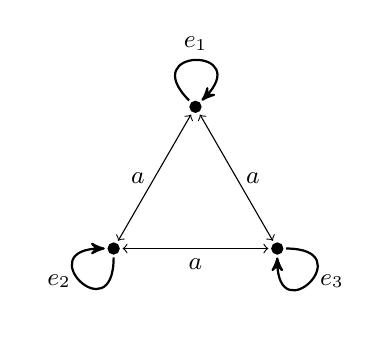
\begin{tikzpicture}[<->,shorten <=1pt,shorten >=1pt,label distance=0mm, font=\small]
\tikzstyle{vertex}=[circle, fill=black, draw=black, inner sep = 0.05cm]

\node[vertex] (1) at (90:1.2cm) {};
\node[vertex] (2) at (210:1.2cm) {};
\node[vertex] (3) at (-30:1.2cm) {};

\draw (1) to node[midway, right] {$a$} (3);
\draw (2) to node[midway, below] {$a$} (3);
\draw (2) to node[midway, left] {$a$} (1);

\Loop[dist=1cm,dir=NO,label=$e_1$,labelstyle=above](1);
\Loop[dist=1cm,dir=SOWE,label=$e_2$,labelstyle=left](2);
\Loop[dist=1cm,dir=SOEA,label=$e_3$,labelstyle=right](3);

\end{tikzpicture}
}      \\[15mm]

\end{longtable}
\end{center}

\section[Four fragment identity]{Atoms: four fragment identity}

\begin{center}
\begin{longtable}{l|c|c}
  atom table & RA  & QRNA \\ \hline && \\[-4mm]  \endhead 
  \hline \endfoot

$
\begin{array}{|c|cccc|} \hline
\#69 & e_1 & e_2 & e_3 & e_4 \\ \hline
e_1 & e_1 & 0 & 0 & 0 \\
e_2 & 0 & e_2 & 0 & 0 \\
e_3 & 0 & 0 & e_3 & 0 \\
e_4 & 0 & 0 & 0 & e_4 \\ \hline
\end{array}
$
%identity: {'a', 'c', 'b', 'd'}
%[('c', 'c'), ('b', 'b'), ('d', 'd')]
 & yes
 & \begin{tabular}{c} not simple: \\ $\#2_{\le 3} \times \#2_{\le 3} \times \#2_{\le 3} \times \#2_{\le 3}$ \end{tabular}       \\[15mm]

\end{longtable}
\end{center}

\section[Atomic identity and three symmetric]{Atoms: atomic identity and three symmetric}

\begin{center}
\begin{longtable}{l|c|c}
  atom table & RA  & QRNA \\ \hline && \\[-4mm]  \endhead 
  \hline \endfoot 
 
$
\begin{array}{|c|cccc|} \hline
\#70 & \id & a & b & c \\ \hline
\id & \id & a & b & c \\
a & a & \id & 0 & 0 \\
b & b & 0 & \id & 0 \\
c & c & 0 & 0 & \id \\ \hline
\end{array}
$
%identity: {'a'}
%[('c', 'c'), ('b', 'b'), ('d', 'd')]
 & no  
 & no      \\[15mm]

$
\begin{array}{|c|cccc|} \hline
\#71 & \id & a & b & c \\ \hline
\id & \id & a & b & c \\
a & a & \id \join a & 0 & 0 \\
b & b & 0 & \id & 0 \\
c & c & 0 & 0 & \id \\ \hline
\end{array}
$
%identity: {'a'}
%[('c', 'c'), ('b', 'b'), ('d', 'd')]
 & no  
 & no      \\[15mm]

$
\begin{array}{|c|cccc|} \hline
\#72 & \id & a & b & c \\ \hline
\id & \id & a & b & c \\
a & a & \id \join b & a & 0 \\
b & b & a & \id & 0 \\
c & c & 0 & 0 & \id \\ \hline
\end{array}
$
%identity: {'a'}
%[('c', 'c'), ('b', 'b'), ('d', 'd')]
 & no  
 & no      \\[15mm]

$
\begin{array}{|c|cccc|} \hline
\#73 & \id & a & b & c \\ \hline
\id & \id & a & b & c \\
a & a & -c & a & 0 \\
b & b & a & \id & 0 \\
c & c & 0 & 0 & \id \\ \hline
\end{array}
$
%identity: {'a'}
%[('c', 'c'), ('b', 'b'), ('d', 'd')]
 & no  
 & no      \\[15mm]

$
\begin{array}{|c|cccc|} \hline
\#74 & \id & a & b & c \\ \hline
\id & \id & a & b & c \\
a & a & -a & a & a \\
b & b & a & \id & 0 \\
c & c & a & 0 & \id \\ \hline
\end{array}
$
%identity: {'a'}
%[('c', 'c'), ('b', 'b'), ('d', 'd')]
 & no  
 & \adjustbox{valign=c, max height=1.7cm}{
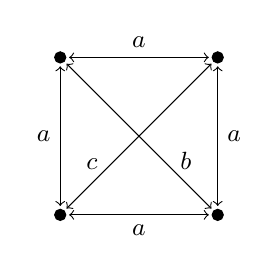
\begin{tikzpicture}[<->,shorten <=1pt,shorten >=1pt,label distance=0mm, font=\small]
\tikzstyle{vertex}=[circle, fill=black, draw=black, inner sep = 0.05cm]

\node[vertex] (1) at (-1,1cm) {};
\node[vertex] (2) at (1,1cm) {};
\node[vertex] (3) at (1,-1cm) {};
\node[vertex] (4) at (-1,-1cm) {};

\draw (1) to node[midway, above] {$a$} (2);
\draw (2) to node[midway, right] {$a$} (3);
\draw (3) to node[midway, below] {$a$} (4);
\draw (1) to node[midway, left] {$a$} (4);
\draw (1) to node[label={[label distance=-1mm, pos=0.75]45:$b$}] {} (3);
\draw (2) to node[label={[label distance=-1mm, pos=0.75]135:$c$}] {} (4);

\end{tikzpicture}
}     \\[15mm]

$
\begin{array}{|c|cccc|} \hline
\#75 & \id & a & b & c \\ \hline
\id & \id & a & b & c \\
a & a & \top & a & a \\
b & b & a & \id & 0 \\
c & c & a & 0 & \id \\ \hline
\end{array}
$
%identity: {'a'}
%[('c', 'c'), ('b', 'b'), ('d', 'd')]
 & no  
 & \adjustbox{valign=c, max height=1.7cm}{
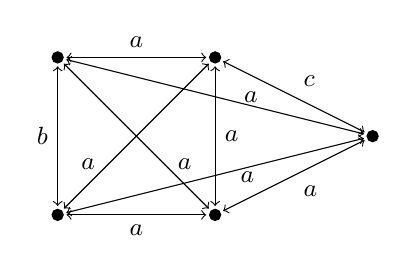
\begin{tikzpicture}[<->,shorten <=1pt,shorten >=1pt,label distance=0mm, font=\small]
\tikzstyle{vertex}=[circle, fill=black, draw=black, inner sep = 0.05cm]

\node[vertex] (1) at (-1,1cm) {};
\node[vertex] (2) at (1,1cm) {};
\node[vertex] (3) at (1,-1cm) {};
\node[vertex] (4) at (-1,-1cm) {};
\node[vertex] (5) at (3,0cm) {};

\draw (1) to node[midway, above] {$a$} (2);
\draw (2) to node[midway, right] {$a$} (3);
\draw (3) to node[midway, below] {$a$} (4);
\draw (1) to node[midway, left] {$b$} (4);
\draw (1) to node[label={[label distance=-1mm, pos=0.75]45:$a$}] {} (3);
\draw (2) to node[label={[label distance=-1mm, pos=0.75]135:$a$}] {} (4);
\draw (5) to node[midway, above right] {$c$} (2);
\draw (5) to node[label={[label distance=-1mm, pos=0.35]150:$a$}] {} (1);
\draw (5) to node[label={[label distance=-0.5mm, pos=0.35]-150:$a$}] {} (4);
\draw (5) to node[midway, below right] {$a$} (3);

\end{tikzpicture}
}     \\[15mm]

$
\begin{array}{|c|cccc|} \hline
\#76 & \id & a & b & c \\ \hline
\id & \id & a & b & c \\
a & a & \id \join a & b & 0 \\
b & b & b & \id \join a & 0 \\
c & c & 0 & 0 & \id \\ \hline
\end{array}
$
%identity: {'a'}
%[('c', 'c'), ('b', 'b'), ('d', 'd')]
 & no  
 & no      \\[15mm]

$
\begin{array}{|c|cccc|} \hline
\#77 & \id & a & b & c \\ \hline
\id & \id & a & b & c \\
a & a & \id \join b & a \join b & 0 \\
b & b & a \join b & \id \join a & 0 \\
c & c & 0 & 0 & \id \\ \hline
\end{array}
$
%identity: {'a'}
%[('c', 'c'), ('b', 'b'), ('d', 'd')]
 & no  
 & no      \\[15mm]

$
\begin{array}{|c|cccc|} \hline
\#78 & \id & a & b & c \\ \hline
\id & \id & a & b & c \\
a & a & -c & a \join b & 0 \\
b & b & a \join b & \id \join a & 0 \\
c & c & 0 & 0 & \id \\ \hline
\end{array}
$
%identity: {'a'}
%[('c', 'c'), ('b', 'b'), ('d', 'd')]
 & no  
 & no      \\[15mm]

$
\begin{array}{|c|cccc|} \hline
\#79 & \id & a & b & c \\ \hline
\id & \id & a & b & c \\
a & a & \id \join c & b & a \\
b & b & b & \id \join a & 0 \\
c & c & a & 0 & \id \\ \hline
\end{array}
$
%identity: {'a'}
%[('c', 'c'), ('b', 'b'), ('d', 'd')]
 & no  
 & no      \\[15mm]

$
\begin{array}{|c|cccc|} \hline
\#80 & \id & a & b & c \\ \hline
\id & \id & a & b & c \\
a & a & -b & b & a \\
b & b & b & \id \join a & 0 \\
c & c & a & 0 & \id \\ \hline
\end{array}
$
%identity: {'a'}
%[('c', 'c'), ('b', 'b'), ('d', 'd')]
 & no  
 & no      \\[15mm]

$
\begin{array}{|c|cccc|} \hline
\#81 & \id & a & b & c \\ \hline
\id & \id & a & b & c \\
a & a & -a & a \join b & a \\
b & b & a \join b & \id \join a & 0 \\
c & c & a & 0 & \id \\ \hline
\end{array}
$
%identity: {'a'}
%[('c', 'c'), ('b', 'b'), ('d', 'd')]
 & no  
 & no      \\[15mm]

$
\begin{array}{|c|cccc|} \hline
\#82 & \id & a & b & c \\ \hline
\id & \id & a & b & c \\
a & a & \top & a \join b & a \\
b & b & a \join b & \id \join a & 0 \\
c & c & a & 0 & \id \\ \hline
\end{array}
$
%identity: {'a'}
%[('c', 'c'), ('b', 'b'), ('d', 'd')]
 & no  
 & \adjustbox{valign=c, max height=1.7cm}{
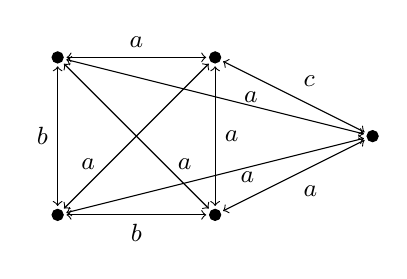
\begin{tikzpicture}[<->,shorten <=1pt,shorten >=1pt,label distance=0mm, font=\small]
\tikzstyle{vertex}=[circle, fill=black, draw=black, inner sep = 0.05cm]

\node[vertex] (1) at (-1,1cm) {};
\node[vertex] (2) at (1,1cm) {};
\node[vertex] (3) at (1,-1cm) {};
\node[vertex] (4) at (-1,-1cm) {};
\node[vertex] (5) at (3,0cm) {};

\draw (1) to node[midway, above] {$a$} (2);
\draw (2) to node[midway, right] {$a$} (3);
\draw (3) to node[midway, below] {$b$} (4);
\draw (1) to node[midway, left] {$b$} (4);
\draw (1) to node[label={[label distance=-1mm, pos=0.75]45:$a$}] {} (3);
\draw (2) to node[label={[label distance=-1mm, pos=0.75]135:$a$}] {} (4);
\draw (5) to node[midway, above right] {$c$} (2);
\draw (5) to node[label={[label distance=-1mm, pos=0.35]150:$a$}] {} (1);
\draw (5) to node[label={[label distance=-0.5mm, pos=0.35]-150:$a$}] {} (4);
\draw (5) to node[midway, below right] {$a$} (3);

\end{tikzpicture}
}      \\[15mm]

$
\begin{array}{|c|cccc|} \hline
\#83 & \id & a & b & c \\ \hline
\id & \id & a & b & c \\
a & a & \id & c & b \\
b & b & c & \id & a \\
c & c & b & a & \id \\ \hline
\end{array}
$
%identity: {'a'}
%[('c', 'c'), ('b', 'b'), ('d', 'd')]
 & \begin{tabular}{c} yes \\ $25_{65}$ \\ $\RRA$ \end{tabular} 
 & \adjustbox{valign=c, max height=1.7cm}{
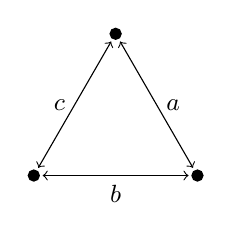
\begin{tikzpicture}[<->,shorten <=1pt,shorten >=1pt,label distance=0mm, font=\small]
\tikzstyle{vertex}=[circle, fill=black, draw=black, inner sep = 0.05cm]

\node[vertex] (1) at (90:1.2cm) {};
\node[vertex] (2) at (210:1.2cm) {};
\node[vertex] (3) at (-30:1.2cm) {};

\draw (1) to node[midway, right] {$a$} (3);
\draw (3) to node[midway, below] {$b$} (2);
\draw (1) to node[midway, left] {$c$} (2);

\end{tikzpicture}
}      \\[15mm]

$
\begin{array}{|c|cccc|} \hline
\#84 & \id & a & b & c \\ \hline
\id & \id & a & b & c \\
a & a & \id \join a & c & b \\
b & b & c & \id & a \\
c & c & b & a & \id \\ \hline
\end{array}
$
%identity: {'a'}
%[('c', 'c'), ('b', 'b'), ('d', 'd')]
 & no  
 & no     \\[15mm]

$
\begin{array}{|c|cccc|} \hline
\#85 & \id & a & b & c \\ \hline
\id & \id & a & b & c \\
a & a & \id \join b & a \join c & b \\
b & b & a \join c & \id & a \\
c & c & b & a & \id \\ \hline
\end{array}
$
%identity: {'a'}
%[('c', 'c'), ('b', 'b'), ('d', 'd')]
 & no  
 & \adjustbox{valign=c, max height=1.7cm}{
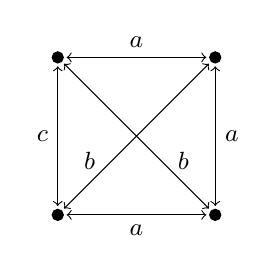
\begin{tikzpicture}[<->,shorten <=1pt,shorten >=1pt,label distance=0mm, font=\small]
\tikzstyle{vertex}=[circle, fill=black, draw=black, inner sep = 0.05cm]

\node[vertex] (1) at (-1,1cm) {};
\node[vertex] (2) at (1,1cm) {};
\node[vertex] (3) at (1,-1cm) {};
\node[vertex] (4) at (-1,-1cm) {};

\draw (1) to node[midway, above] {$a$} (2);
\draw (2) to node[midway, right] {$a$} (3);
\draw (3) to node[midway, below] {$a$} (4);
\draw (1) to node[midway, left] {$c$} (4);
\draw (1) to node[label={[label distance=-1mm, pos=0.75]45:$b$}] {} (3);
\draw (2) to node[label={[label distance=-1mm, pos=0.75]135:$b$}] {} (4);

\end{tikzpicture}
}      \\[15mm]

$
\begin{array}{|c|cccc|} \hline
\#86 & \id & a & b & c \\ \hline
\id & \id & a & b & c \\
a & a & -c & a \join c & b \\
b & b & a \join c & \id & a \\
c & c & b & a & \id \\ \hline
\end{array}
$
%identity: {'a'}
%[('c', 'c'), ('b', 'b'), ('d', 'd')]
 & no  
 & no      \\[15mm]

$
\begin{array}{|c|cccc|} \hline
\#87 & \id & a & b & c \\ \hline
\id & \id & a & b & c \\
a & a & -a & a \join c & a \join b \\
b & b & a \join c & \id & a \\
c & c & a \join b & a & \id \\ \hline
\end{array}
$
%identity: {'a'}
%[('c', 'c'), ('b', 'b'), ('d', 'd')]
 & no  
 & no      \\[15mm]

$
\begin{array}{|c|cccc|} \hline
\#88 & \id & a & b & c \\ \hline
\id & \id & a & b & c \\
a & a & \top & a \join c & a \join b \\
b & b & a \join c & \id & a \\
c & c & a \join b & a & \id \\ \hline
\end{array}
$
%identity: {'a'}
%[('c', 'c'), ('b', 'b'), ('d', 'd')]
 & no  
 & \adjustbox{valign=c, max height=1.7cm}{
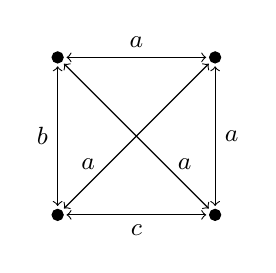
\begin{tikzpicture}[<->,shorten <=1pt,shorten >=1pt,label distance=0mm, font=\small]
\tikzstyle{vertex}=[circle, fill=black, draw=black, inner sep = 0.05cm]

\node[vertex] (1) at (-1,1cm) {};
\node[vertex] (2) at (1,1cm) {};
\node[vertex] (3) at (1,-1cm) {};
\node[vertex] (4) at (-1,-1cm) {};

\draw (1) to node[midway, above] {$a$} (2);
\draw (2) to node[midway, right] {$a$} (3);
\draw (3) to node[midway, below] {$c$} (4);
\draw (1) to node[midway, left] {$b$} (4);
\draw (1) to node[label={[label distance=-1mm, pos=0.75]45:$a$}] {} (3);
\draw (2) to node[label={[label distance=-1mm, pos=0.75]135:$a$}] {} (4);

\end{tikzpicture}
}      \\[15mm]

$
\begin{array}{|c|cccc|} \hline
\#89 & \id & a & b & c \\ \hline
\id & \id & a & b & c \\
a & a & \id \join a & b \join c & b \\
b & b & b \join c & \id \join a & a \\
c & c & b & a & \id \\ \hline
\end{array}
$
%identity: {'a'}
%[('c', 'c'), ('b', 'b'), ('d', 'd')]
 & \begin{tabular}{c} yes \\ $26_{65}$ \\ $\RRA$ \end{tabular} 
 & \adjustbox{valign=c, max height=1.7cm}{
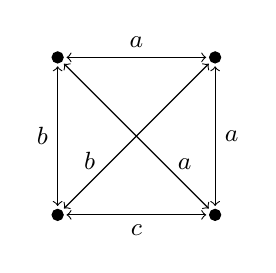
\begin{tikzpicture}[<->,shorten <=1pt,shorten >=1pt,label distance=0mm, font=\small]
\tikzstyle{vertex}=[circle, fill=black, draw=black, inner sep = 0.05cm]

\node[vertex] (1) at (-1,1cm) {};
\node[vertex] (2) at (1,1cm) {};
\node[vertex] (3) at (1,-1cm) {};
\node[vertex] (4) at (-1,-1cm) {};

\draw (1) to node[midway, above] {$a$} (2);
\draw (2) to node[midway, right] {$a$} (3);
\draw (3) to node[midway, below] {$c$} (4);
\draw (1) to node[midway, left] {$b$} (4);
\draw (1) to node[label={[label distance=-1mm, pos=0.75]45:$a$}] {} (3);
\draw (2) to node[label={[label distance=-1mm, pos=0.75]135:$b$}] {} (4);

\end{tikzpicture}
}      \\[15mm]

$
\begin{array}{|c|cccc|} \hline
\#90 & \id & a & b & c \\ \hline
\id & \id & a & b & c \\
a & a & \id \join b & \div & b \\
b & b & \div & \id \join a & a \\
c & c & b & a & \id \\ \hline
\end{array}
$
%identity: {'a'}
%[('c', 'c'), ('b', 'b'), ('d', 'd')]
 & no  
 & no       \\[15mm]

$
\begin{array}{|c|cccc|} \hline
\#91 & \id & a & b & c \\ \hline
\id & \id & a & b & c \\
a & a & -c & \div & b \\
b & b & \div & \id \join a & a \\
c & c & b & a & \id \\ \hline
\end{array}
$
%identity: {'a'}
%[('c', 'c'), ('b', 'b'), ('d', 'd')]
 & no  
 & \adjustbox{valign=c, max height=1.7cm}{
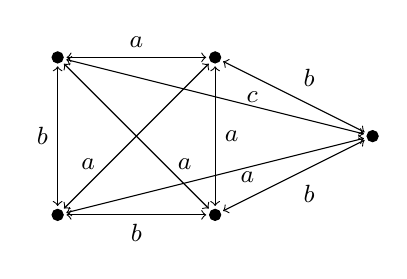
\begin{tikzpicture}[<->,shorten <=1pt,shorten >=1pt,label distance=0mm, font=\small]
\tikzstyle{vertex}=[circle, fill=black, draw=black, inner sep = 0.05cm]

\node[vertex] (1) at (-1,1cm) {};
\node[vertex] (2) at (1,1cm) {};
\node[vertex] (3) at (1,-1cm) {};
\node[vertex] (4) at (-1,-1cm) {};
\node[vertex] (5) at (3,0cm) {};

\draw (1) to node[midway, above] {$a$} (2);
\draw (2) to node[midway, right] {$a$} (3);
\draw (3) to node[midway, below] {$b$} (4);
\draw (1) to node[midway, left] {$b$} (4);
\draw (1) to node[label={[label distance=-1mm, pos=0.75]45:$a$}] {} (3);
\draw (2) to node[label={[label distance=-1mm, pos=0.75]135:$a$}] {} (4);
\draw (5) to node[midway, above right] {$b$} (2);
\draw (5) to node[label={[label distance=-1mm, pos=0.35]150:$c$}] {} (1);
\draw (5) to node[label={[label distance=-0.5mm, pos=0.35]-150:$a$}] {} (4);
\draw (5) to node[midway, below right] {$b$} (3);

\end{tikzpicture}
}      \\[15mm]

$
\begin{array}{|c|cccc|} \hline
\#92 & \id & a & b & c \\ \hline
\id & \id & a & b & c \\
a & a & \id \join c & b \join c & a \join b \\
b & b & b \join c & \id \join a & a \\
c & c & a \join b & a & \id \\ \hline
\end{array}
$
%identity: {'a'}
%[('c', 'c'), ('b', 'b'), ('d', 'd')]
 & no  
 & no      \\[15mm]

$
\begin{array}{|c|cccc|} \hline
\#93 & \id & a & b & c \\ \hline
\id & \id & a & b & c \\
a & a & -b & b \join c & a \join b \\
b & b & b \join c & \id \join a & a \\
c & c & a \join b & a & \id \\ \hline
\end{array}
$
%identity: {'a'}
%[('c', 'c'), ('b', 'b'), ('d', 'd')]
 & no  
 & no      \\[15mm]

$
\begin{array}{|c|cccc|} \hline
\#94 & \id & a & b & c \\ \hline
\id & \id & a & b & c \\
a & a & -a & \div & a \join b \\
b & b & \div & \id \join a & a \\
c & c & a \join b & a & \id \\ \hline
\end{array}
$
%identity: {'a'}
%[('c', 'c'), ('b', 'b'), ('d', 'd')]
 & no  
 & \adjustbox{valign=c, max height=1.7cm}{
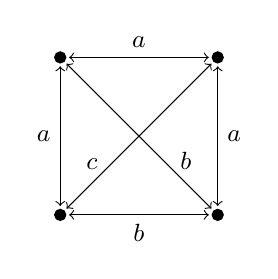
\begin{tikzpicture}[<->,shorten <=1pt,shorten >=1pt,label distance=0mm, font=\small]
\tikzstyle{vertex}=[circle, fill=black, draw=black, inner sep = 0.05cm]

\node[vertex] (1) at (-1,1cm) {};
\node[vertex] (2) at (1,1cm) {};
\node[vertex] (3) at (1,-1cm) {};
\node[vertex] (4) at (-1,-1cm) {};

\draw (1) to node[midway, above] {$a$} (2);
\draw (2) to node[midway, right] {$a$} (3);
\draw (3) to node[midway, below] {$b$} (4);
\draw (1) to node[midway, left] {$a$} (4);
\draw (1) to node[label={[label distance=-1mm, pos=0.75]45:$b$}] {} (3);
\draw (2) to node[label={[label distance=-1mm, pos=0.75]135:$c$}] {} (4);

\end{tikzpicture}
}      \\[15mm]

$
\begin{array}{|c|cccc|} \hline
\#95 & \id & a & b & c \\ \hline
\id & \id & a & b & c \\
a & a & \top & \div & a \join b \\
b & b & \div & \id \join a & a \\
c & c & a \join b & a & \id \\ \hline
\end{array}
$
%identity: {'a'}
%[('c', 'c'), ('b', 'b'), ('d', 'd')]
 & no  
 & \adjustbox{valign=c, max height=1.7cm}{
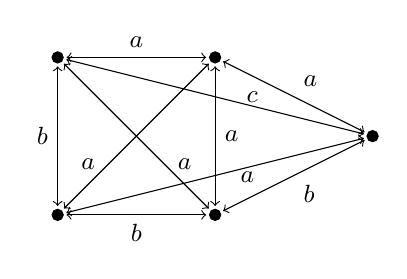
\begin{tikzpicture}[<->,shorten <=1pt,shorten >=1pt,label distance=0mm, font=\small]
\tikzstyle{vertex}=[circle, fill=black, draw=black, inner sep = 0.05cm]

\node[vertex] (1) at (-1,1cm) {};
\node[vertex] (2) at (1,1cm) {};
\node[vertex] (3) at (1,-1cm) {};
\node[vertex] (4) at (-1,-1cm) {};
\node[vertex] (5) at (3,0cm) {};

\draw (1) to node[midway, above] {$a$} (2);
\draw (2) to node[midway, right] {$a$} (3);
\draw (3) to node[midway, below] {$b$} (4);
\draw (1) to node[midway, left] {$b$} (4);
\draw (1) to node[label={[label distance=-1mm, pos=0.75]45:$a$}] {} (3);
\draw (2) to node[label={[label distance=-1mm, pos=0.75]135:$a$}] {} (4);
\draw (5) to node[midway, above right] {$a$} (2);
\draw (5) to node[label={[label distance=-1mm, pos=0.35]150:$c$}] {} (1);
\draw (5) to node[label={[label distance=-0.5mm, pos=0.35]-150:$a$}] {} (4);
\draw (5) to node[midway, below right] {$b$} (3);

\end{tikzpicture}
}      \\[15mm]

$
\begin{array}{|c|cccc|} \hline
\#96 & \id & a & b & c \\ \hline
\id & \id & a & b & c \\
a & a & \id & b & c \\
b & b & b & \id \join a & 0 \\
c & c & c & 0 & \id \join a \\ \hline
\end{array}
$
%identity: {'a'}
%[('c', 'c'), ('b', 'b'), ('d', 'd')]
 & no  
 & no      \\[15mm]

$
\begin{array}{|c|cccc|} \hline
\#97 & \id & a & b & c \\ \hline
\id & \id & a & b & c \\
a & a & \id \join a & b & c \\
b & b & b & \id \join a & 0 \\
c & c & c & 0 & \id \join a \\ \hline
\end{array}
$
%identity: {'a'}
%[('c', 'c'), ('b', 'b'), ('d', 'd')]
 & no  
 & no      \\[15mm]

$
\begin{array}{|c|cccc|} \hline
\#98 & \id & a & b & c \\ \hline
\id & \id & a & b & c \\
a & a & \id \join b & a \join b & c \\
b & b & a \join b & \id \join a & 0 \\
c & c & c & 0 & \id \join a \\ \hline
\end{array}
$
%identity: {'a'}
%[('c', 'c'), ('b', 'b'), ('d', 'd')]
 & no  
 & no      \\[15mm]

$
\begin{array}{|c|cccc|} \hline
\#99 & \id & a & b & c \\ \hline
\id & \id & a & b & c \\
a & a & -c & a \join b & c \\
b & b & a \join b & \id \join a & 0 \\
c & c & c & 0 & \id \join a \\ \hline
\end{array}
$
%identity: {'a'}
%[('c', 'c'), ('b', 'b'), ('d', 'd')]
 & no  
 & no      \\[15mm]

$
\begin{array}{|c|cccc|} \hline
\#100 & \id & a & b & c \\ \hline
\id & \id & a & b & c \\
a & a & -a & a \join b & a \join c \\
b & b & a \join b & \id \join a & 0 \\
c & c & a \join c & 0 & \id \join a \\ \hline
\end{array}
$
%identity: {'a'}
%[('c', 'c'), ('b', 'b'), ('d', 'd')]
 & no  
 & no      \\[15mm]

$
\begin{array}{|c|cccc|} \hline
\#101 & \id & a & b & c \\ \hline
\id & \id & a & b & c \\
a & a & \top & a \join b & a \join c \\
b & b & a \join b & \id \join a & 0 \\
c & c & a \join c & 0 & \id \join a \\ \hline
\end{array}
$
%identity: {'a'}
%[('c', 'c'), ('b', 'b'), ('d', 'd')]
 & no  
 & \adjustbox{valign=c, max height=1.6cm}{$
\left[ \begin{array}{cccccc}
\id & a & a & b & a & a \\ 
a & \id & a & a & c & a \\ 
a & a & \id & b & a & a \\ 
b & a & b & \id & a & a \\ 
a & c & a & a & \id & c \\ 
a & a & a & a & c & \id
\end{array}\right]
$}      \\[15mm]

$
\begin{array}{|c|cccc|} \hline
\#102 & \id & a & b & c \\ \hline
\id & \id & a & b & c \\
a & a & \id & b \join c & b \join c \\
b & b & b \join c & \id \join a & a \\
c & c & b \join c & a & \id \join a \\ \hline
\end{array}
$
%identity: {'a'}
%[('c', 'c'), ('b', 'b'), ('d', 'd')]
 & no  
 & \adjustbox{valign=c, max height=1.7cm}{
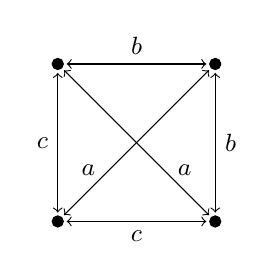
\begin{tikzpicture}[<->,shorten <=1pt,shorten >=1pt,label distance=0mm, font=\small]
\tikzstyle{vertex}=[circle, fill=black, draw=black, inner sep = 0.05cm]

\node[vertex] (1) at (-1,1cm) {};
\node[vertex] (2) at (1,1cm) {};
\node[vertex] (3) at (1,-1cm) {};
\node[vertex] (4) at (-1,-1cm) {};

\draw (1) to node[midway, above] {$b$} (2);
\draw (2) to node[midway, right] {$b$} (3);
\draw (3) to node[midway, below] {$c$} (4);
\draw (1) to node[midway, left] {$c$} (4);
\draw (1) to node[label={[label distance=-1mm, pos=0.75]45:$a$}] {} (3);
\draw (2) to node[label={[label distance=-1mm, pos=0.75]135:$a$}] {} (4);

\end{tikzpicture}
}      \\[15mm]

$
\begin{array}{|c|cccc|} \hline
\#103 & \id & a & b & c \\ \hline
\id & \id & a & b & c \\
a & a & \id \join a & b \join c & b \join c \\
b & b & b \join c & \id \join a & a \\
c & c & b \join c & a & \id \join a \\ \hline
\end{array}
$
%identity: {'a'}
%[('c', 'c'), ('b', 'b'), ('d', 'd')]
 & \begin{tabular}{c} yes \\ $28_{65}$ \\ $\RRA$ \end{tabular} 
 & \adjustbox{valign=c, max height=1.7cm}{
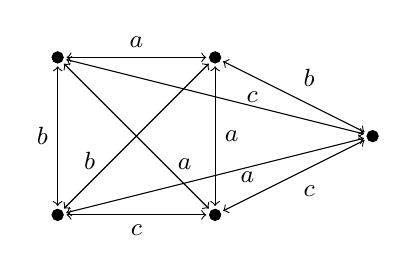
\begin{tikzpicture}[<->,shorten <=1pt,shorten >=1pt,label distance=0mm, font=\small]
\tikzstyle{vertex}=[circle, fill=black, draw=black, inner sep = 0.05cm]

\node[vertex] (1) at (-1,1cm) {};
\node[vertex] (2) at (1,1cm) {};
\node[vertex] (3) at (1,-1cm) {};
\node[vertex] (4) at (-1,-1cm) {};
\node[vertex] (5) at (3,0cm) {};

\draw (1) to node[midway, above] {$a$} (2);
\draw (2) to node[midway, right] {$a$} (3);
\draw (3) to node[midway, below] {$c$} (4);
\draw (1) to node[midway, left] {$b$} (4);
\draw (1) to node[label={[label distance=-1mm, pos=0.75]45:$a$}] {} (3);
\draw (2) to node[label={[label distance=-1mm, pos=0.75]135:$b$}] {} (4);
\draw (5) to node[midway, above right] {$b$} (2);
\draw (5) to node[label={[label distance=-1mm, pos=0.35]150:$c$}] {} (1);
\draw (5) to node[label={[label distance=-0.5mm, pos=0.35]-150:$a$}] {} (4);
\draw (5) to node[midway, below right] {$c$} (3);

\end{tikzpicture}
}      \\[15mm]

$
\begin{array}{|c|cccc|} \hline
\#104 & \id & a & b & c \\ \hline
\id & \id & a & b & c \\
a & a & \id \join b & \div & b \join c \\
b & b & \div & \id \join a & a \\
c & c & b \join c & a & \id \join a \\ \hline
\end{array}
$
%identity: {'a'}
%[('c', 'c'), ('b', 'b'), ('d', 'd')]
 & no  
 & no      \\[15mm]

$
\begin{array}{|c|cccc|} \hline
\#105 & \id & a & b & c \\ \hline
\id & \id & a & b & c \\
a & a & -c & \div & b \join c \\
b & b & \div & \id \join a & a \\
c & c & b \join c & a & \id \join a \\ \hline
\end{array}
$
%identity: {'a'}
%[('c', 'c'), ('b', 'b'), ('d', 'd')]
 & no  
 & \adjustbox{valign=c, max height=1.7cm}{
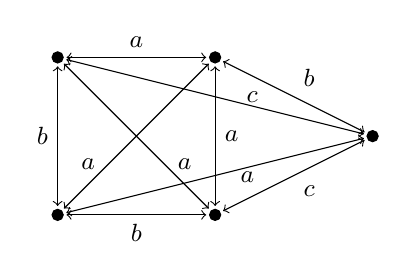
\begin{tikzpicture}[<->,shorten <=1pt,shorten >=1pt,label distance=0mm, font=\small]
\tikzstyle{vertex}=[circle, fill=black, draw=black, inner sep = 0.05cm]

\node[vertex] (1) at (-1,1cm) {};
\node[vertex] (2) at (1,1cm) {};
\node[vertex] (3) at (1,-1cm) {};
\node[vertex] (4) at (-1,-1cm) {};
\node[vertex] (5) at (3,0cm) {};

\draw (1) to node[midway, above] {$a$} (2);
\draw (2) to node[midway, right] {$a$} (3);
\draw (3) to node[midway, below] {$b$} (4);
\draw (1) to node[midway, left] {$b$} (4);
\draw (1) to node[label={[label distance=-1mm, pos=0.75]45:$a$}] {} (3);
\draw (2) to node[label={[label distance=-1mm, pos=0.75]135:$a$}] {} (4);
\draw (5) to node[midway, above right] {$b$} (2);
\draw (5) to node[label={[label distance=-1mm, pos=0.35]150:$c$}] {} (1);
\draw (5) to node[label={[label distance=-0.5mm, pos=0.35]-150:$a$}] {} (4);
\draw (5) to node[midway, below right] {$c$} (3);

\end{tikzpicture}
}      \\[15mm]

$
\begin{array}{|c|cccc|} \hline
\#106 & \id & a & b & c \\ \hline
\id & \id & a & b & c \\
a & a & -a & \div & \div \\
b & b & \div & \id \join a & a \\
c & c & \div & a & \id \join a \\ \hline
\end{array}
$
%identity: {'a'}
%[('c', 'c'), ('b', 'b'), ('d', 'd')]
 & no  
 & \adjustbox{valign=c, max height=1.7cm}{
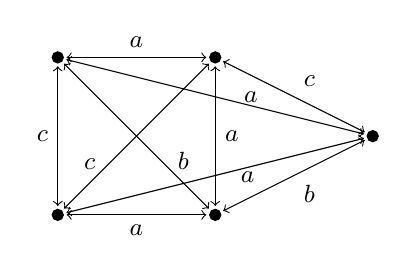
\begin{tikzpicture}[<->,shorten <=1pt,shorten >=1pt,label distance=0mm, font=\small]
\tikzstyle{vertex}=[circle, fill=black, draw=black, inner sep = 0.05cm]

\node[vertex] (1) at (-1,1cm) {};
\node[vertex] (2) at (1,1cm) {};
\node[vertex] (3) at (1,-1cm) {};
\node[vertex] (4) at (-1,-1cm) {};
\node[vertex] (5) at (3,0cm) {};

\draw (1) to node[midway, above] {$a$} (2);
\draw (2) to node[midway, right] {$a$} (3);
\draw (3) to node[midway, below] {$a$} (4);
\draw (1) to node[midway, left] {$c$} (4);
\draw (1) to node[label={[label distance=-1mm, pos=0.75]45:$b$}] {} (3);
\draw (2) to node[label={[label distance=-1mm, pos=0.75]135:$c$}] {} (4);
\draw (5) to node[midway, above right] {$c$} (2);
\draw (5) to node[label={[label distance=-1mm, pos=0.35]150:$a$}] {} (1);
\draw (5) to node[label={[label distance=-0.5mm, pos=0.35]-150:$a$}] {} (4);
\draw (5) to node[midway, below right] {$b$} (3);

\end{tikzpicture}
}      \\[15mm]

$
\begin{array}{|c|cccc|} \hline
\#107 & \id & a & b & c \\ \hline
\id & \id & a & b & c \\
a & a & \top & \div & \div \\
b & b & \div & \id \join a & a \\
c & c & \div & a & \id \join a \\ \hline
\end{array}
$
%identity: {'a'}
%[('c', 'c'), ('b', 'b'), ('d', 'd')]
 & \begin{tabular}{c} yes \\ $32_{65}$ \\ $\RRA$ \end{tabular} 
 & \adjustbox{valign=c, max height=1.7cm}{
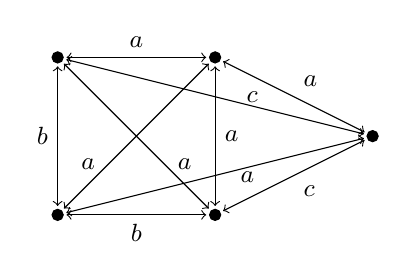
\begin{tikzpicture}[<->,shorten <=1pt,shorten >=1pt,label distance=0mm, font=\small]
\tikzstyle{vertex}=[circle, fill=black, draw=black, inner sep = 0.05cm]

\node[vertex] (1) at (-1,1cm) {};
\node[vertex] (2) at (1,1cm) {};
\node[vertex] (3) at (1,-1cm) {};
\node[vertex] (4) at (-1,-1cm) {};
\node[vertex] (5) at (3,0cm) {};

\draw (1) to node[midway, above] {$a$} (2);
\draw (2) to node[midway, right] {$a$} (3);
\draw (3) to node[midway, below] {$b$} (4);
\draw (1) to node[midway, left] {$b$} (4);
\draw (1) to node[label={[label distance=-1mm, pos=0.75]45:$a$}] {} (3);
\draw (2) to node[label={[label distance=-1mm, pos=0.75]135:$a$}] {} (4);
\draw (5) to node[midway, above right] {$a$} (2);
\draw (5) to node[label={[label distance=-1mm, pos=0.35]150:$c$}] {} (1);
\draw (5) to node[label={[label distance=-0.5mm, pos=0.35]-150:$a$}] {} (4);
\draw (5) to node[midway, below right] {$c$} (3);

\end{tikzpicture}
}      \\[15mm]

$
\begin{array}{|c|cccc|} \hline
\#108 & \id & a & b & c \\ \hline
\id & \id & a & b & c \\
a & a & \id \join a & 0 & 0 \\
b & b & 0 & \id \join b & 0 \\
c & c & 0 & 0 & \id \\ \hline
\end{array}
$
%identity: {'a'}
%[('c', 'c'), ('b', 'b'), ('d', 'd')]
 & no  
 & no      \\[15mm]

$
\begin{array}{|c|cccc|} \hline
\#109 & \id & a & b & c \\ \hline
\id & \id & a & b & c \\
a & a & -c & a & 0 \\
b & b & a & \id \join b & 0 \\
c & c & 0 & 0 & \id \\ \hline
\end{array}
$
%identity: {'a'}
%[('c', 'c'), ('b', 'b'), ('d', 'd')]
 & no  
 & no      \\[15mm]

$
\begin{array}{|c|cccc|} \hline
\#110 & \id & a & b & c \\ \hline
\id & \id & a & b & c \\
a & a & \id \join c & 0 & a \\
b & b & 0 & \id \join b & 0 \\
c & c & a & 0 & \id \\ \hline
\end{array}
$
%identity: {'a'}
%[('c', 'c'), ('b', 'b'), ('d', 'd')]
 & no  
 & no      \\[15mm]

$
\begin{array}{|c|cccc|} \hline
\#111 & \id & a & b & c \\ \hline
\id & \id & a & b & c \\
a & a & -b & 0 & a \\
b & b & 0 & \id \join b & 0 \\
c & c & a & 0 & \id \\ \hline
\end{array}
$
%identity: {'a'}
%[('c', 'c'), ('b', 'b'), ('d', 'd')]
 & no  
 & no      \\[15mm]

$
\begin{array}{|c|cccc|} \hline
\#112 & \id & a & b & c \\ \hline
\id & \id & a & b & c \\
a & a & -a & a & a \\
b & b & a & \id \join b & 0 \\
c & c & a & 0 & \id \\ \hline
\end{array}
$
%identity: {'a'}
%[('c', 'c'), ('b', 'b'), ('d', 'd')]
 & no  
 & \adjustbox{valign=c, max height=1.7cm}{
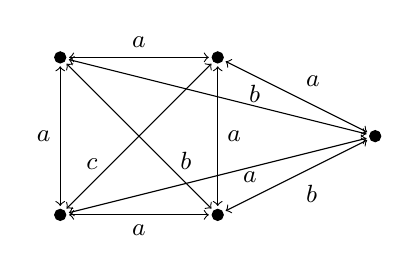
\begin{tikzpicture}[<->,shorten <=1pt,shorten >=1pt,label distance=0mm, font=\small]
\tikzstyle{vertex}=[circle, fill=black, draw=black, inner sep = 0.05cm]

\node[vertex] (1) at (-1,1cm) {};
\node[vertex] (2) at (1,1cm) {};
\node[vertex] (3) at (1,-1cm) {};
\node[vertex] (4) at (-1,-1cm) {};
\node[vertex] (5) at (3,0cm) {};

\draw (1) to node[midway, above] {$a$} (2);
\draw (2) to node[midway, right] {$a$} (3);
\draw (3) to node[midway, below] {$a$} (4);
\draw (1) to node[midway, left] {$a$} (4);
\draw (1) to node[label={[label distance=-1mm, pos=0.75]45:$b$}] {} (3);
\draw (2) to node[label={[label distance=-1mm, pos=0.75]135:$c$}] {} (4);
\draw (5) to node[midway, above right] {$a$} (2);
\draw (5) to node[label={[label distance=-1mm, pos=0.35]150:$b$}] {} (1);
\draw (5) to node[label={[label distance=-0.5mm, pos=0.35]-150:$a$}] {} (4);
\draw (5) to node[midway, below right] {$b$} (3);

\end{tikzpicture}
}      \\[15mm]

$
\begin{array}{|c|cccc|} \hline
\#113 & \id & a & b & c \\ \hline
\id & \id & a & b & c \\
a & a & \top & a & a \\
b & b & a & \id \join b & 0 \\
c & c & a & 0 & \id \\ \hline
\end{array}
$
%identity: {'a'}
%[('c', 'c'), ('b', 'b'), ('d', 'd')]
 & no  
 & \adjustbox{valign=c, max height=1.6cm}{$
\left[ \begin{array}{cccccc}
\id & a & a & b & a & b \\ 
a & \id & a & a & c & a \\ 
a & a & \id & a & a & a \\ 
b & a & a & \id & a & b \\ 
a & c & a & a & \id & a \\ 
b & a & a & b & a & \id
\end{array}\right]
$}
      \\[15mm]

$
\begin{array}{|c|cccc|} \hline
\#114 & \id & a & b & c \\ \hline
\id & \id & a & b & c \\
a & a & -c & a \join b & 0 \\
b & b & a \join b & -c & 0 \\
c & c & 0 & 0 & \id \\ \hline
\end{array}
$
%identity: {'a'}
%[('c', 'c'), ('b', 'b'), ('d', 'd')]
 & no  
 & \adjustbox{valign=c, max height=1.7cm}{
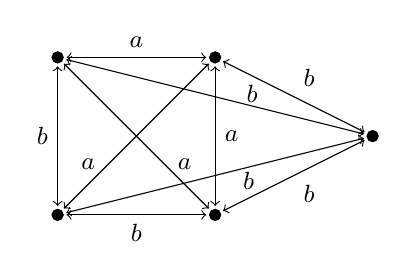
\begin{tikzpicture}[<->,shorten <=1pt,shorten >=1pt,label distance=0mm, font=\small]
\tikzstyle{vertex}=[circle, fill=black, draw=black, inner sep = 0.05cm]

\node[vertex] (1) at (-1,1cm) {};
\node[vertex] (2) at (1,1cm) {};
\node[vertex] (3) at (1,-1cm) {};
\node[vertex] (4) at (-1,-1cm) {};
\node[vertex] (5) at (3,0cm) {};

\draw (1) to node[midway, above] {$a$} (2);
\draw (2) to node[midway, right] {$a$} (3);
\draw (3) to node[midway, below] {$b$} (4);
\draw (1) to node[midway, left] {$b$} (4);
\draw (1) to node[label={[label distance=-1mm, pos=0.75]45:$a$}] {} (3);
\draw (2) to node[label={[label distance=-1mm, pos=0.75]135:$a$}] {} (4);
\draw (5) to node[midway, above right] {$b$} (2);
\draw (5) to node[label={[label distance=-1mm, pos=0.35]150:$b$}] {} (1);
\draw (5) to node[label={[label distance=-0.5mm, pos=0.35]-150:$b$}] {} (4);
\draw (5) to node[midway, below right] {$b$} (3);

\end{tikzpicture}
}      \\[15mm]

$
\begin{array}{|c|cccc|} \hline
\#115 & \id & a & b & c \\ \hline
\id & \id & a & b & c \\
a & a & \id \join c & b & a \\
b & b & b & -c & 0 \\
c & c & a & 0 & \id \\ \hline
\end{array}
$
%identity: {'a'}
%[('c', 'c'), ('b', 'b'), ('d', 'd')]
 & no  
 & no      \\[15mm]

$
\begin{array}{|c|cccc|} \hline
\#116 & \id & a & b & c \\ \hline
\id & \id & a & b & c \\
a & a & -b & b & a \\
b & b & b & -c & 0 \\
c & c & a & 0 & \id \\ \hline
\end{array}
$
%identity: {'a'}
%[('c', 'c'), ('b', 'b'), ('d', 'd')]
 & no  
 & no      \\[15mm]

$
\begin{array}{|c|cccc|} \hline
\#117 & \id & a & b & c \\ \hline
\id & \id & a & b & c \\
a & a & -a & a \join b & a \\
b & b & a \join b & -c & 0 \\
c & c & a & 0 & \id \\ \hline
\end{array}
$
%identity: {'a'}
%[('c', 'c'), ('b', 'b'), ('d', 'd')]
 & no  
 & no      \\[15mm]

$
\begin{array}{|c|cccc|} \hline
\#118 & \id & a & b & c \\ \hline
\id & \id & a & b & c \\
a & a & \top & a \join b & a \\
b & b & a \join b & -c & 0 \\
c & c & a & 0 & \id \\ \hline
\end{array}
$
%identity: {'a'}
%[('c', 'c'), ('b', 'b'), ('d', 'd')]
 & no  
 & \adjustbox{valign=c, max height=1.6cm}{$
\left[ \begin{array}{cccccc}
\id & a & a & b & a & b \\ 
a & \id & a & a & c & a \\ 
a & a & \id & b & a & b \\ 
b & a & b & \id & a & b \\ 
a & c & a & a & \id & a \\ 
b & a & b & b & a & \id
\end{array}\right]
$}     \\[15mm]

$
\begin{array}{|c|cccc|} \hline
\#119 & \id & a & b & c \\ \hline
\id & \id & a & b & c \\
a & a & \id \join a & c & b \\
b & b & c & \id \join b & a \\
c & c & b & a & \id \\ \hline
\end{array}
$
%identity: {'a'}
%[('c', 'c'), ('b', 'b'), ('d', 'd')]
 & no  
 & no      \\[15mm]

$
\begin{array}{|c|cccc|} \hline
\#120 & \id & a & b & c \\ \hline
\id & \id & a & b & c \\
a & a & -c & a \join c & b \\
b & b & a \join c & \id \join b & a \\
c & c & b & a & \id \\ \hline
\end{array}
$
%identity: {'a'}
%[('c', 'c'), ('b', 'b'), ('d', 'd')]
 & no  
 & no      \\[15mm]

$
\begin{array}{|c|cccc|} \hline
\#121 & \id & a & b & c \\ \hline
\id & \id & a & b & c \\
a & a & \id \join c & c & a \join b \\
b & b & c & \id \join b & a \\
c & c & a \join b & a & \id \\ \hline
\end{array}
$
%identity: {'a'}
%[('c', 'c'), ('b', 'b'), ('d', 'd')]
 & no  
 & no      \\[15mm]

$
\begin{array}{|c|cccc|} \hline
\#122 & \id & a & b & c \\ \hline
\id & \id & a & b & c \\
a & a & -b & c & a \join b \\
b & b & c & \id \join b & a \\
c & c & a \join b & a & \id \\ \hline
\end{array}
$
%identity: {'a'}
%[('c', 'c'), ('b', 'b'), ('d', 'd')]
 & no  
 & no      \\[15mm]

$
\begin{array}{|c|cccc|} \hline
\#123 & \id & a & b & c \\ \hline
\id & \id & a & b & c \\
a & a & -a & a \join c & a \join b \\
b & b & a \join c & \id \join b & a \\
c & c & a \join b & a & \id \\ \hline
\end{array}
$
%identity: {'a'}
%[('c', 'c'), ('b', 'b'), ('d', 'd')]
 & no  
 & no       \\[15mm]

$
\begin{array}{|c|cccc|} \hline
\#124 & \id & a & b & c \\ \hline
\id & \id & a & b & c \\
a & a & \top & a \join c & a \join b \\
b & b & a \join c & \id \join b & a \\
c & c & a \join b & a & \id \\ \hline
\end{array}
$
%identity: {'a'}
%[('c', 'c'), ('b', 'b'), ('d', 'd')]
 & no  
 & \adjustbox{valign=c, max height=1.7cm}{
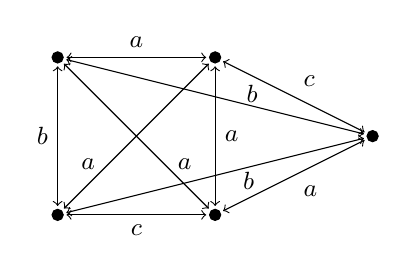
\begin{tikzpicture}[<->,shorten <=1pt,shorten >=1pt,label distance=0mm, font=\small]
\tikzstyle{vertex}=[circle, fill=black, draw=black, inner sep = 0.05cm]

\node[vertex] (1) at (-1,1cm) {};
\node[vertex] (2) at (1,1cm) {};
\node[vertex] (3) at (1,-1cm) {};
\node[vertex] (4) at (-1,-1cm) {};
\node[vertex] (5) at (3,0cm) {};

\draw (1) to node[midway, above] {$a$} (2);
\draw (2) to node[midway, right] {$a$} (3);
\draw (3) to node[midway, below] {$c$} (4);
\draw (1) to node[midway, left] {$b$} (4);
\draw (1) to node[label={[label distance=-1mm, pos=0.75]45:$a$}] {} (3);
\draw (2) to node[label={[label distance=-1mm, pos=0.75]135:$a$}] {} (4);
\draw (5) to node[midway, above right] {$c$} (2);
\draw (5) to node[label={[label distance=-1mm, pos=0.35]150:$b$}] {} (1);
\draw (5) to node[label={[label distance=-0.5mm, pos=0.35]-150:$b$}] {} (4);
\draw (5) to node[midway, below right] {$a$} (3);

\end{tikzpicture}
}      \\[15mm]

$
\begin{array}{|c|cccc|} \hline
\#125 & \id & a & b & c \\ \hline
\id & \id & a & b & c \\
a & a & -c & \div & b \\
b & b & \div & -c & a \\
c & c & b & a & \id \\ \hline
\end{array}
$
%identity: {'a'}
%[('c', 'c'), ('b', 'b'), ('d', 'd')]
 & \begin{tabular}{c} yes \\ $27_{65}$ \\ $\RRA$ \end{tabular} 
 & \adjustbox{valign=c, max height=1.7cm}{
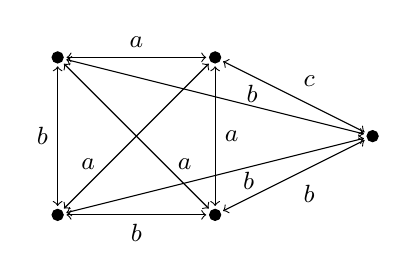
\begin{tikzpicture}[<->,shorten <=1pt,shorten >=1pt,label distance=0mm, font=\small]
\tikzstyle{vertex}=[circle, fill=black, draw=black, inner sep = 0.05cm]

\node[vertex] (1) at (-1,1cm) {};
\node[vertex] (2) at (1,1cm) {};
\node[vertex] (3) at (1,-1cm) {};
\node[vertex] (4) at (-1,-1cm) {};
\node[vertex] (5) at (3,0cm) {};

\draw (1) to node[midway, above] {$a$} (2);
\draw (2) to node[midway, right] {$a$} (3);
\draw (3) to node[midway, below] {$b$} (4);
\draw (1) to node[midway, left] {$b$} (4);
\draw (1) to node[label={[label distance=-1mm, pos=0.75]45:$a$}] {} (3);
\draw (2) to node[label={[label distance=-1mm, pos=0.75]135:$a$}] {} (4);
\draw (5) to node[midway, above right] {$c$} (2);
\draw (5) to node[label={[label distance=-1mm, pos=0.35]150:$b$}] {} (1);
\draw (5) to node[label={[label distance=-0.5mm, pos=0.35]-150:$b$}] {} (4);
\draw (5) to node[midway, below right] {$b$} (3);

\end{tikzpicture}
}      \\[15mm]

$
\begin{array}{|c|cccc|} \hline
\#126 & \id & a & b & c \\ \hline
\id & \id & a & b & c \\
a & a & \id \join c & b \join c & a \join b \\
b & b & b \join c & -c & a \\
c & c & a \join b & a & \id \\ \hline
\end{array}
$
%identity: {'a'}
%[('c', 'c'), ('b', 'b'), ('d', 'd')]
 & no  
 & no      \\[15mm]

$
\begin{array}{|c|cccc|} \hline
\#127 & \id & a & b & c \\ \hline
\id & \id & a & b & c \\
a & a & -b & b \join c & a \join b \\
b & b & b \join c & -c & a \\
c & c & a \join b & a & \id \\ \hline
\end{array}
$
%identity: {'a'}
%[('c', 'c'), ('b', 'b'), ('d', 'd')]
 & no  
 & no       \\[15mm]

$
\begin{array}{|c|cccc|} \hline
\#128 & \id & a & b & c \\ \hline
\id & \id & a & b & c \\
a & a & -a & \div & a \join b \\
b & b & \div & -c & a \\
c & c & a \join b & a & \id \\ \hline
\end{array}
$
%identity: {'a'}
%[('c', 'c'), ('b', 'b'), ('d', 'd')]
 & no  
 & \adjustbox{valign=c, max height=1.7cm}{
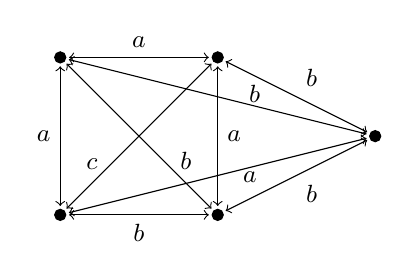
\begin{tikzpicture}[<->,shorten <=1pt,shorten >=1pt,label distance=0mm, font=\small]
\tikzstyle{vertex}=[circle, fill=black, draw=black, inner sep = 0.05cm]

\node[vertex] (1) at (-1,1cm) {};
\node[vertex] (2) at (1,1cm) {};
\node[vertex] (3) at (1,-1cm) {};
\node[vertex] (4) at (-1,-1cm) {};
\node[vertex] (5) at (3,0cm) {};

\draw (1) to node[midway, above] {$a$} (2);
\draw (2) to node[midway, right] {$a$} (3);
\draw (3) to node[midway, below] {$b$} (4);
\draw (1) to node[midway, left] {$a$} (4);
\draw (1) to node[label={[label distance=-1mm, pos=0.75]45:$b$}] {} (3);
\draw (2) to node[label={[label distance=-1mm, pos=0.75]135:$c$}] {} (4);
\draw (5) to node[midway, above right] {$b$} (2);
\draw (5) to node[label={[label distance=-1mm, pos=0.35]150:$b$}] {} (1);
\draw (5) to node[label={[label distance=-0.5mm, pos=0.35]-150:$a$}] {} (4);
\draw (5) to node[midway, below right] {$b$} (3);

\end{tikzpicture}
}      \\[15mm]

$
\begin{array}{|c|cccc|} \hline
\#129 & \id & a & b & c \\ \hline
\id & \id & a & b & c \\
a & a & \top & \div & a \join b \\
b & b & \div & -c & a \\
c & c & a \join b & a & \id \\ \hline
\end{array}
$
%identity: {'a'}
%[('c', 'c'), ('b', 'b'), ('d', 'd')]
 & no  
 & \adjustbox{valign=c, max height=1.7cm}{
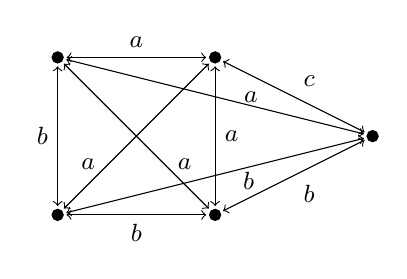
\begin{tikzpicture}[<->,shorten <=1pt,shorten >=1pt,label distance=0mm, font=\small]
\tikzstyle{vertex}=[circle, fill=black, draw=black, inner sep = 0.05cm]

\node[vertex] (1) at (-1,1cm) {};
\node[vertex] (2) at (1,1cm) {};
\node[vertex] (3) at (1,-1cm) {};
\node[vertex] (4) at (-1,-1cm) {};
\node[vertex] (5) at (3,0cm) {};

\draw (1) to node[midway, above] {$a$} (2);
\draw (2) to node[midway, right] {$a$} (3);
\draw (3) to node[midway, below] {$b$} (4);
\draw (1) to node[midway, left] {$b$} (4);
\draw (1) to node[label={[label distance=-1mm, pos=0.75]45:$a$}] {} (3);
\draw (2) to node[label={[label distance=-1mm, pos=0.75]135:$a$}] {} (4);
\draw (5) to node[midway, above right] {$c$} (2);
\draw (5) to node[label={[label distance=-1mm, pos=0.35]150:$a$}] {} (1);
\draw (5) to node[label={[label distance=-0.5mm, pos=0.35]-150:$b$}] {} (4);
\draw (5) to node[midway, below right] {$b$} (3);

\end{tikzpicture}
}      \\[15mm]

$
\begin{array}{|c|cccc|} \hline
\#130 & \id & a & b & c \\ \hline
\id & \id & a & b & c \\
a & a & \id \join a & 0 & c \\
b & b & 0 & \id \join b & 0 \\
c & c & c & 0 & \id \join a \\ \hline
\end{array}
$
%identity: {'a'}
%[('c', 'c'), ('b', 'b'), ('d', 'd')]
 & no  
 & no     \\[15mm]

$
\begin{array}{|c|cccc|} \hline
\#131 & \id & a & b & c \\ \hline
\id & \id & a & b & c \\
a & a & \id \join b & a & c \\
b & b & a & \id \join b & 0 \\
c & c & c & 0 & \id \join a \\ \hline
\end{array}
$
%identity: {'a'}
%[('c', 'c'), ('b', 'b'), ('d', 'd')]
 & no  
 & no      \\[15mm]

$
\begin{array}{|c|cccc|} \hline
\#132 & \id & a & b & c \\ \hline
\id & \id & a & b & c \\
a & a & -c & a & c \\
b & b & a & \id \join b & 0 \\
c & c & c & 0 & \id \join a \\ \hline
\end{array}
$
%identity: {'a'}
%[('c', 'c'), ('b', 'b'), ('d', 'd')]
 & no  
 & no      \\[15mm]

$
\begin{array}{|c|cccc|} \hline
\#133 & \id & a & b & c \\ \hline
\id & \id & a & b & c \\
a & a & \id \join c & 0 & a \join c \\
b & b & 0 & \id \join b & 0 \\
c & c & a \join c & 0 & \id \join a \\ \hline
\end{array}
$
%identity: {'a'}
%[('c', 'c'), ('b', 'b'), ('d', 'd')]
 & no  
 & no      \\[15mm]

$
\begin{array}{|c|cccc|} \hline
\#134 & \id & a & b & c \\ \hline
\id & \id & a & b & c \\
a & a & -b & 0 & a \join c \\
b & b & 0 & \id \join b & 0 \\
c & c & a \join c & 0 & \id \join a \\ \hline
\end{array}
$
%identity: {'a'}
%[('c', 'c'), ('b', 'b'), ('d', 'd')]
 & no  
 & no      \\[15mm]

$
\begin{array}{|c|cccc|} \hline
\#135 & \id & a & b & c \\ \hline
\id & \id & a & b & c \\
a & a & -a & a & a \join c \\
b & b & a & \id \join b & 0 \\
c & c & a \join c & 0 & \id \join a \\ \hline
\end{array}
$
%identity: {'a'}
%[('c', 'c'), ('b', 'b'), ('d', 'd')]
 & no  
 & no      \\[15mm]

$
\begin{array}{|c|cccc|} \hline
\#136 & \id & a & b & c \\ \hline
\id & \id & a & b & c \\
a & a & \top & a & a \join c \\
b & b & a & \id \join b & 0 \\
c & c & a \join c & 0 & \id \join a \\ \hline
\end{array}
$
%identity: {'a'}
%[('c', 'c'), ('b', 'b'), ('d', 'd')]
 & no  
 & \adjustbox{valign=c, max height=1.6cm}{$
\left[ \begin{array}{cccccc}
\id & a & b & a & a & b \\ 
a & \id & a & c & a & a \\ 
b & a & \id & a & a & b \\ 
a & c & a & \id & c & a \\ 
a & a & a & c & \id & a \\ 
b & a & b & a & a & \id
\end{array}\right]
$}      \\[15mm]

$
\begin{array}{|c|cccc|} \hline
\#137 & \id & a & b & c \\ \hline
\id & \id & a & b & c \\
a & a & \id & b & c \\
b & b & b & -c & 0 \\
c & c & c & 0 & \id \join a \\ \hline
\end{array}
$
%identity: {'a'}
%[('c', 'c'), ('b', 'b'), ('d', 'd')]
 & no  
 & no      \\[15mm]

$
\begin{array}{|c|cccc|} \hline
\#138 & \id & a & b & c \\ \hline
\id & \id & a & b & c \\
a & a & \id \join a & b & c \\
b & b & b & -c & 0 \\
c & c & c & 0 & \id \join a \\ \hline
\end{array}
$
%identity: {'a'}
%[('c', 'c'), ('b', 'b'), ('d', 'd')]
 & no  
 & no      \\[15mm]

$
\begin{array}{|c|cccc|} \hline
\#139 & \id & a & b & c \\ \hline
\id & \id & a & b & c \\
a & a & \id \join b & a \join b & c \\
b & b & a \join b & -c & 0 \\
c & c & c & 0 & \id \join a \\ \hline
\end{array}
$
%identity: {'a'}
%[('c', 'c'), ('b', 'b'), ('d', 'd')]
 & no  
 & no      \\[15mm]

$
\begin{array}{|c|cccc|} \hline
\#140 & \id & a & b & c \\ \hline
\id & \id & a & b & c \\
a & a & -c & a \join b & c \\
b & b & a \join b & -c & 0 \\
c & c & c & 0 & \id \join a \\ \hline
\end{array}
$
%identity: {'a'}
%[('c', 'c'), ('b', 'b'), ('d', 'd')]
 & no  
 & no      \\[15mm]

$
\begin{array}{|c|cccc|} \hline
\#141 & \id & a & b & c \\ \hline
\id & \id & a & b & c \\
a & a & \id \join c & b & a \join c \\
b & b & b & -c & 0 \\
c & c & a \join c & 0 & \id \join a \\ \hline
\end{array}
$
%identity: {'a'}
%[('c', 'c'), ('b', 'b'), ('d', 'd')]
 & no  
 & no      \\[15mm]

$
\begin{array}{|c|cccc|} \hline
\#142 & \id & a & b & c \\ \hline
\id & \id & a & b & c \\
a & a & -b & b & a \join c \\
b & b & b & -c & 0 \\
c & c & a \join c & 0 & \id \join a \\ \hline
\end{array}
$
%identity: {'a'}
%[('c', 'c'), ('b', 'b'), ('d', 'd')]
 & no  
 & no      \\[15mm]

$
\begin{array}{|c|cccc|} \hline
\#143 & \id & a & b & c \\ \hline
\id & \id & a & b & c \\
a & a & -a & a \join b & a \join c \\
b & b & a \join b & -c & 0 \\
c & c & a \join c & 0 & \id \join a \\ \hline
\end{array}
$
%identity: {'a'}
%[('c', 'c'), ('b', 'b'), ('d', 'd')]
 & no  
 & no      \\[15mm]

$
\begin{array}{|c|cccc|} \hline
\#144 & \id & a & b & c \\ \hline
\id & \id & a & b & c \\
a & a & \top & a \join b & a \join c \\
b & b & a \join b & -c & 0 \\
c & c & a \join c & 0 & \id \join a \\ \hline
\end{array}
$
%identity: {'a'}
%[('c', 'c'), ('b', 'b'), ('d', 'd')]
 & no  
 & \adjustbox{valign=c, max height=1.6cm}{$
\left[ \begin{array}{ccccccc}
\id & a & a & b & a & a & b \\ 
a & \id & a & a & c & a & a \\ 
a & a & \id & b & a & a & b \\ 
b & a & b & \id & a & a & b \\ 
a & c & a & a & \id & c & a \\ 
a & a & a & a & c & \id & a \\ 
b & a & b & b & a & a & \id
\end{array}\right]
$}      \\[15mm]

$
\begin{array}{|c|cccc|} \hline
\#145 & \id & a & b & c \\ \hline
\id & \id & a & b & c \\
a & a & \id \join a & c & b \join c \\
b & b & c & \id \join b & a \\
c & c & b \join c & a & \id \join a \\ \hline
\end{array}
$
%identity: {'a'}
%[('c', 'c'), ('b', 'b'), ('d', 'd')]
 & no  
 & no      \\[15mm]

$
\begin{array}{|c|cccc|} \hline
\#146 & \id & a & b & c \\ \hline
\id & \id & a & b & c \\
a & a & \id \join b & a \join c & b \join c \\
b & b & a \join c & \id \join b & a \\
c & c & b \join c & a & \id \join a \\ \hline
\end{array}
$
%identity: {'a'}
%[('c', 'c'), ('b', 'b'), ('d', 'd')]
 & no  
 & no      \\[15mm]

$
\begin{array}{|c|cccc|} \hline
\#147 & \id & a & b & c \\ \hline
\id & \id & a & b & c \\
a & a & -c & a \join c & b \join c \\
b & b & a \join c & \id \join b & a \\
c & c & b \join c & a & \id \join a \\ \hline
\end{array}
$
%identity: {'a'}
%[('c', 'c'), ('b', 'b'), ('d', 'd')]
 & no  
 & \adjustbox{valign=c, max height=1.7cm}{
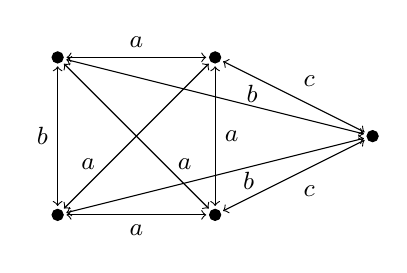
\begin{tikzpicture}[<->,shorten <=1pt,shorten >=1pt,label distance=0mm, font=\small]
\tikzstyle{vertex}=[circle, fill=black, draw=black, inner sep = 0.05cm]

\node[vertex] (1) at (-1,1cm) {};
\node[vertex] (2) at (1,1cm) {};
\node[vertex] (3) at (1,-1cm) {};
\node[vertex] (4) at (-1,-1cm) {};
\node[vertex] (5) at (3,0cm) {};

\draw (1) to node[midway, above] {$a$} (2);
\draw (2) to node[midway, right] {$a$} (3);
\draw (3) to node[midway, below] {$a$} (4);
\draw (1) to node[midway, left] {$b$} (4);
\draw (1) to node[label={[label distance=-1mm, pos=0.75]45:$a$}] {} (3);
\draw (2) to node[label={[label distance=-1mm, pos=0.75]135:$a$}] {} (4);
\draw (5) to node[midway, above right] {$c$} (2);
\draw (5) to node[label={[label distance=-1mm, pos=0.35]150:$b$}] {} (1);
\draw (5) to node[label={[label distance=-0.5mm, pos=0.35]-150:$b$}] {} (4);
\draw (5) to node[midway, below right] {$c$} (3);

\end{tikzpicture}
}      \\[15mm]

$
\begin{array}{|c|cccc|} \hline
\#148 & \id & a & b & c \\ \hline
\id & \id & a & b & c \\
a & a & \id \join c & c & \div \\
b & b & c & \id \join b & a \\
c & c & \div & a & \id \join a \\ \hline
\end{array}
$
%identity: {'a'}
%[('c', 'c'), ('b', 'b'), ('d', 'd')]
 & no  
 & no      \\[15mm]

$
\begin{array}{|c|cccc|} \hline
\#149 & \id & a & b & c \\ \hline
\id & \id & a & b & c \\
a & a & -b & c & \div \\
b & b & c & \id \join b & a \\
c & c & \div & a & \id \join a \\ \hline
\end{array}
$
%identity: {'a'}
%[('c', 'c'), ('b', 'b'), ('d', 'd')]
 & no  
 & no      \\[15mm]

$
\begin{array}{|c|cccc|} \hline
\#150 & \id & a & b & c \\ \hline
\id & \id & a & b & c \\
a & a & -a & a \join c & \div \\
b & b & a \join c & \id \join b & a \\
c & c & \div & a & \id \join a \\ \hline
\end{array}
$
%identity: {'a'}
%[('c', 'c'), ('b', 'b'), ('d', 'd')]
 & no  
 & \adjustbox{valign=c, max height=1.7cm}{
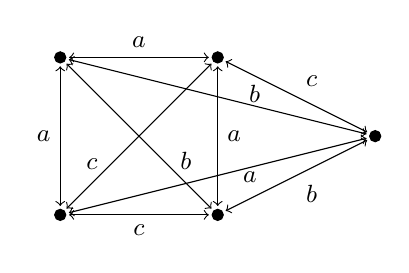
\begin{tikzpicture}[<->,shorten <=1pt,shorten >=1pt,label distance=0mm, font=\small]
\tikzstyle{vertex}=[circle, fill=black, draw=black, inner sep = 0.05cm]

\node[vertex] (1) at (-1,1cm) {};
\node[vertex] (2) at (1,1cm) {};
\node[vertex] (3) at (1,-1cm) {};
\node[vertex] (4) at (-1,-1cm) {};
\node[vertex] (5) at (3,0cm) {};

\draw (1) to node[midway, above] {$a$} (2);
\draw (2) to node[midway, right] {$a$} (3);
\draw (3) to node[midway, below] {$c$} (4);
\draw (1) to node[midway, left] {$a$} (4);
\draw (1) to node[label={[label distance=-1mm, pos=0.75]45:$b$}] {} (3);
\draw (2) to node[label={[label distance=-1mm, pos=0.75]135:$c$}] {} (4);
\draw (5) to node[midway, above right] {$c$} (2);
\draw (5) to node[label={[label distance=-1mm, pos=0.35]150:$b$}] {} (1);
\draw (5) to node[label={[label distance=-0.5mm, pos=0.35]-150:$a$}] {} (4);
\draw (5) to node[midway, below right] {$b$} (3);

\end{tikzpicture}
}      \\[15mm]

$
\begin{array}{|c|cccc|} \hline
\#151 & \id & a & b & c \\ \hline
\id & \id & a & b & c \\
a & a & \top & a \join c & \div \\
b & b & a \join c & \id \join b & a \\
c & c & \div & a & \id \join a \\ \hline
\end{array}
$
%identity: {'a'}
%[('c', 'c'), ('b', 'b'), ('d', 'd')]
 & \begin{tabular}{c} yes \\ $30_{65}$ \\ $\RRA$ \end{tabular} 
 & \adjustbox{valign=c, max height=1.6cm}{$
\left[ \begin{array}{cccccc}
\id & a & a & b & c & b \\ 
a & \id & a & a & a & c \\ 
a & a & \id & a & b & c \\ 
b & a & a & \id & a & b \\ 
c & a & b & a & \id & a \\ 
b & c & c & b & a & \id
\end{array}\right]
$}     \\[15mm]

$
\begin{array}{|c|cccc|} \hline
\#152 & \id & a & b & c \\ \hline
\id & \id & a & b & c \\
a & a & \id & b \join c & b \join c \\
b & b & b \join c & -c & a \\
c & c & b \join c & a & \id \join a \\ \hline
\end{array}
$
%identity: {'a'}
%[('c', 'c'), ('b', 'b'), ('d', 'd')]
 & no  
 & no      \\[15mm]

$
\begin{array}{|c|cccc|} \hline
\#153 & \id & a & b & c \\ \hline
\id & \id & a & b & c \\
a & a & \id \join a & b \join c & b \join c \\
b & b & b \join c & -c & a \\
c & c & b \join c & a & \id \join a \\ \hline
\end{array}
$
%identity: {'a'}
%[('c', 'c'), ('b', 'b'), ('d', 'd')]
 & no  
 & \adjustbox{valign=c, max height=1.7cm}{
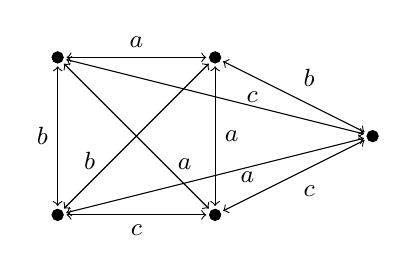
\begin{tikzpicture}[<->,shorten <=1pt,shorten >=1pt,label distance=0mm, font=\small]
\tikzstyle{vertex}=[circle, fill=black, draw=black, inner sep = 0.05cm]

\node[vertex] (1) at (-1,1cm) {};
\node[vertex] (2) at (1,1cm) {};
\node[vertex] (3) at (1,-1cm) {};
\node[vertex] (4) at (-1,-1cm) {};
\node[vertex] (5) at (3,0cm) {};

\draw (1) to node[midway, above] {$a$} (2);
\draw (2) to node[midway, right] {$a$} (3);
\draw (3) to node[midway, below] {$c$} (4);
\draw (1) to node[midway, left] {$b$} (4);
\draw (1) to node[label={[label distance=-1mm, pos=0.75]45:$a$}] {} (3);
\draw (2) to node[label={[label distance=-1mm, pos=0.75]135:$b$}] {} (4);
\draw (5) to node[midway, above right] {$b$} (2);
\draw (5) to node[label={[label distance=-1mm, pos=0.35]150:$c$}] {} (1);
\draw (5) to node[label={[label distance=-0.5mm, pos=0.35]-150:$a$}] {} (4);
\draw (5) to node[midway, below right] {$c$} (3);

\end{tikzpicture}
}      \\[15mm]

$
\begin{array}{|c|cccc|} \hline
\#154 & \id & a & b & c \\ \hline
\id & \id & a & b & c \\
a & a & \id \join b & \div & b \join c \\
b & b & \div & -c & a \\
c & c & b \join c & a & \id \join a \\ \hline
\end{array}
$
%identity: {'a'}
%[('c', 'c'), ('b', 'b'), ('d', 'd')]
 & no  
 & \adjustbox{valign=c, max height=1.7cm}{
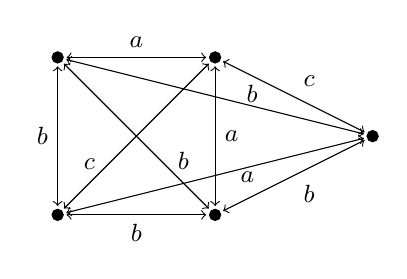
\begin{tikzpicture}[<->,shorten <=1pt,shorten >=1pt,label distance=0mm, font=\small]
\tikzstyle{vertex}=[circle, fill=black, draw=black, inner sep = 0.05cm]

\node[vertex] (1) at (-1,1cm) {};
\node[vertex] (2) at (1,1cm) {};
\node[vertex] (3) at (1,-1cm) {};
\node[vertex] (4) at (-1,-1cm) {};
\node[vertex] (5) at (3,0cm) {};

\draw (1) to node[midway, above] {$a$} (2);
\draw (2) to node[midway, right] {$a$} (3);
\draw (3) to node[midway, below] {$b$} (4);
\draw (1) to node[midway, left] {$b$} (4);
\draw (1) to node[label={[label distance=-1mm, pos=0.75]45:$b$}] {} (3);
\draw (2) to node[label={[label distance=-1mm, pos=0.75]135:$c$}] {} (4);
\draw (5) to node[midway, above right] {$c$} (2);
\draw (5) to node[label={[label distance=-1mm, pos=0.35]150:$b$}] {} (1);
\draw (5) to node[label={[label distance=-0.5mm, pos=0.35]-150:$a$}] {} (4);
\draw (5) to node[midway, below right] {$b$} (3);

\end{tikzpicture}
}      \\[15mm]

$
\begin{array}{|c|cccc|} \hline
\#155 & \id & a & b & c \\ \hline
\id & \id & a & b & c \\
a & a & -c & \div & b \join c \\
b & b & \div & -c & a \\
c & c & b \join c & a & \id \join a \\ \hline
\end{array}
$
%identity: {'a'}
%[('c', 'c'), ('b', 'b'), ('d', 'd')]
 & no  
 & \adjustbox{valign=c, max height=1.6cm}{$
\left[ \begin{array}{cccccc}
\id & a & a & b & c & b \\ 
a & \id & a & a & b & c \\ 
a & a & \id & b & c & b \\ 
b & a & b & \id & a & b \\ 
c & b & c & a & \id & a \\ 
b & c & b & b & a & \id
\end{array}\right]
$}      \\[15mm]

$
\begin{array}{|c|cccc|} \hline
\#156 & \id & a & b & c \\ \hline
\id & \id & a & b & c \\
a & a & \id \join c & b \join c & \div \\
b & b & b \join c & -c & a \\
c & c & \div & a & \id \join a \\ \hline
\end{array}
$
%identity: {'a'}
%[('c', 'c'), ('b', 'b'), ('d', 'd')]
 & no  
 & no      \\[15mm]

$
\begin{array}{|c|cccc|} \hline
\#157 & \id & a & b & c \\ \hline
\id & \id & a & b & c \\
a & a & -b & b \join c & \div \\
b & b & b \join c & -c & a \\
c & c & \div & a & \id \join a \\ \hline
\end{array}
$
%identity: {'a'}
%[('c', 'c'), ('b', 'b'), ('d', 'd')]
 & no  
 & no      \\[15mm]

$
\begin{array}{|c|cccc|} \hline
\#158 & \id & a & b & c \\ \hline
\id & \id & a & b & c \\
a & a & -a & \div & \div \\
b & b & \div & -c & a \\
c & c & \div & a & \id \join a \\ \hline
\end{array}
$
%identity: {'a'}
%[('c', 'c'), ('b', 'b'), ('d', 'd')]
 & no  
 & \adjustbox{valign=c, max height=1.7cm}{
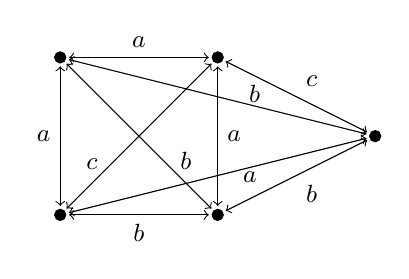
\begin{tikzpicture}[<->,shorten <=1pt,shorten >=1pt,label distance=0mm, font=\small]
\tikzstyle{vertex}=[circle, fill=black, draw=black, inner sep = 0.05cm]

\node[vertex] (1) at (-1,1cm) {};
\node[vertex] (2) at (1,1cm) {};
\node[vertex] (3) at (1,-1cm) {};
\node[vertex] (4) at (-1,-1cm) {};
\node[vertex] (5) at (3,0cm) {};

\draw (1) to node[midway, above] {$a$} (2);
\draw (2) to node[midway, right] {$a$} (3);
\draw (3) to node[midway, below] {$b$} (4);
\draw (1) to node[midway, left] {$a$} (4);
\draw (1) to node[label={[label distance=-1mm, pos=0.75]45:$b$}] {} (3);
\draw (2) to node[label={[label distance=-1mm, pos=0.75]135:$c$}] {} (4);
\draw (5) to node[midway, above right] {$c$} (2);
\draw (5) to node[label={[label distance=-1mm, pos=0.35]150:$b$}] {} (1);
\draw (5) to node[label={[label distance=-0.5mm, pos=0.35]-150:$a$}] {} (4);
\draw (5) to node[midway, below right] {$b$} (3);

\end{tikzpicture}
}      \\[15mm]

$
\begin{array}{|c|cccc|} \hline
\#159 & \id & a & b & c \\ \hline
\id & \id & a & b & c \\
a & a & \top & \div & \div \\
b & b & \div & -c & a \\
c & c & \div & a & \id \join a \\ \hline
\end{array}
$
%identity: {'a'}
%[('c', 'c'), ('b', 'b'), ('d', 'd')]
 & \begin{tabular}{c} yes \\ $33_{65}$ \\ $\RRA$ \end{tabular} 
 & \adjustbox{valign=c, max height=1.6cm}{$
\left[ \begin{array}{cccccc}
\id & a & a & b & c & b \\ 
a & \id & a & a & a & c \\ 
a & a & \id & b & c & b \\ 
b & a & b & \id & a & b \\ 
c & a & c & a & \id & a \\ 
b & c & b & b & a & \id
\end{array}\right]
$}      \\[15mm]

$
\begin{array}{|c|cccc|} \hline
\#160 & \id & a & b & c \\ \hline
\id & \id & a & b & c \\
a & a & -a & a & a \\
b & b & a & \id \join c & b \\
c & c & a & b & \id \\ \hline
\end{array}
$
%identity: {'a'}
%[('c', 'c'), ('b', 'b'), ('d', 'd')]
 & \begin{tabular}{c} yes \\ $1_{65}$ \\ $\RRA$ \end{tabular} 
 & \adjustbox{valign=c, max height=1.7cm}{
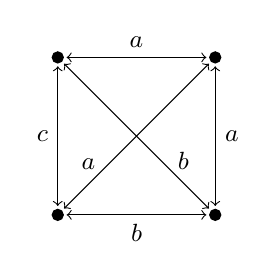
\begin{tikzpicture}[<->,shorten <=1pt,shorten >=1pt,label distance=0mm, font=\small]
\tikzstyle{vertex}=[circle, fill=black, draw=black, inner sep = 0.05cm]

\node[vertex] (1) at (-1,1cm) {};
\node[vertex] (2) at (1,1cm) {};
\node[vertex] (3) at (1,-1cm) {};
\node[vertex] (4) at (-1,-1cm) {};

\draw (1) to node[midway, above] {$a$} (2);
\draw (2) to node[midway, right] {$a$} (3);
\draw (3) to node[midway, below] {$b$} (4);
\draw (1) to node[midway, left] {$c$} (4);
\draw (1) to node[label={[label distance=-1mm, pos=0.75]45:$b$}] {} (3);
\draw (2) to node[label={[label distance=-1mm, pos=0.75]135:$a$}] {} (4);

\end{tikzpicture}
}      \\[15mm]

$
\begin{array}{|c|cccc|} \hline
\#161 & \id & a & b & c \\ \hline
\id & \id & a & b & c \\
a & a & \top & a & a \\
b & b & a & \id \join c & b \\
c & c & a & b & \id \\ \hline
\end{array}
$
%identity: {'a'}
%[('c', 'c'), ('b', 'b'), ('d', 'd')]
 & \begin{tabular}{c} yes \\ $5_{65}$ \\ $\RRA$ \end{tabular} 
 & \adjustbox{valign=c, max height=1.7cm}{
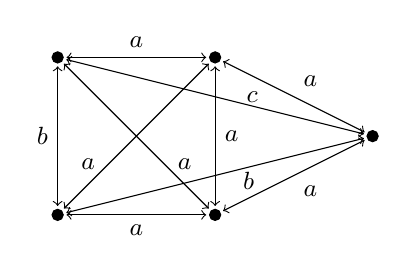
\begin{tikzpicture}[<->,shorten <=1pt,shorten >=1pt,label distance=0mm, font=\small]
\tikzstyle{vertex}=[circle, fill=black, draw=black, inner sep = 0.05cm]

\node[vertex] (1) at (-1,1cm) {};
\node[vertex] (2) at (1,1cm) {};
\node[vertex] (3) at (1,-1cm) {};
\node[vertex] (4) at (-1,-1cm) {};
\node[vertex] (5) at (3,0cm) {};

\draw (1) to node[midway, above] {$a$} (2);
\draw (2) to node[midway, right] {$a$} (3);
\draw (3) to node[midway, below] {$a$} (4);
\draw (1) to node[midway, left] {$b$} (4);
\draw (1) to node[label={[label distance=-1mm, pos=0.75]45:$a$}] {} (3);
\draw (2) to node[label={[label distance=-1mm, pos=0.75]135:$a$}] {} (4);
\draw (5) to node[midway, above right] {$a$} (2);
\draw (5) to node[label={[label distance=-1mm, pos=0.35]150:$c$}] {} (1);
\draw (5) to node[label={[label distance=-0.5mm, pos=0.35]-150:$b$}] {} (4);
\draw (5) to node[midway, below right] {$a$} (3);

\end{tikzpicture}
}      \\[15mm]

$
\begin{array}{|c|cccc|} \hline
\#162 & \id & a & b & c \\ \hline
\id & \id & a & b & c \\
a & a & -b & b & a \\
b & b & b & -b & b \\
c & c & a & b & \id \\ \hline
\end{array}
$
%identity: {'a'}
%[('c', 'c'), ('b', 'b'), ('d', 'd')]
 & \begin{tabular}{c} yes \\ $3_{65}$ \\ $\RRA$ \end{tabular} 
 & \adjustbox{valign=c, max height=1.7cm}{
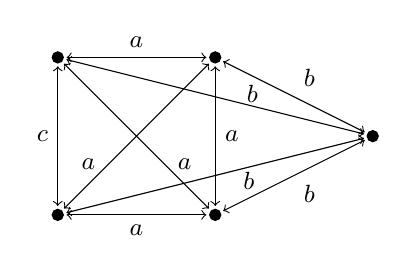
\begin{tikzpicture}[<->,shorten <=1pt,shorten >=1pt,label distance=0mm, font=\small]
\tikzstyle{vertex}=[circle, fill=black, draw=black, inner sep = 0.05cm]

\node[vertex] (1) at (-1,1cm) {};
\node[vertex] (2) at (1,1cm) {};
\node[vertex] (3) at (1,-1cm) {};
\node[vertex] (4) at (-1,-1cm) {};
\node[vertex] (5) at (3,0cm) {};

\draw (1) to node[midway, above] {$a$} (2);
\draw (2) to node[midway, right] {$a$} (3);
\draw (3) to node[midway, below] {$a$} (4);
\draw (1) to node[midway, left] {$c$} (4);
\draw (1) to node[label={[label distance=-1mm, pos=0.75]45:$a$}] {} (3);
\draw (2) to node[label={[label distance=-1mm, pos=0.75]135:$a$}] {} (4);
\draw (5) to node[midway, above right] {$b$} (2);
\draw (5) to node[label={[label distance=-1mm, pos=0.35]150:$b$}] {} (1);
\draw (5) to node[label={[label distance=-0.5mm, pos=0.35]-150:$b$}] {} (4);
\draw (5) to node[midway, below right] {$b$} (3);

\end{tikzpicture}
}      \\[15mm]

$
\begin{array}{|c|cccc|} \hline
\#163 & \id & a & b & c \\ \hline
\id & \id & a & b & c \\
a & a & -a & a \join b & a \\
b & b & a \join b & -b & b \\
c & c & a & b & \id \\ \hline
\end{array}
$
%identity: {'a'}
%[('c', 'c'), ('b', 'b'), ('d', 'd')]
 & \begin{tabular}{c} yes \\ $15_{65}$ \\ $\RRA$ \end{tabular} 
 & \adjustbox{valign=c, max height=1.7cm}{
\begin{tikzpicture}[<->,shorten <=1pt,shorten >=1pt,label distance=0mm, font=\small]
\tikzstyle{vertex}=[circle, fill=black, draw=black, inner sep = 0.05cm]

\node[vertex] (1) at (-1,1cm) {};
\node[vertex] (2) at (1,1cm) {};
\node[vertex] (3) at (1,-1cm) {};
\node[vertex] (4) at (-1,-1cm) {};
\node[vertex] (5) at (3,0cm) {};

\draw (1) to node[midway, above] {$a$} (2);
\draw (2) to node[midway, right] {$a$} (3);
\draw (3) to node[midway, below] {$b$} (4);
\draw (1) to node[midway, left] {$c$} (4);
\draw (1) to node[label={[label distance=-1mm, pos=0.75]45:$b$}] {} (3);
\draw (2) to node[label={[label distance=-1mm, pos=0.75]135:$a$}] {} (4);
\draw (5) to node[midway, above right] {$b$} (2);
\draw (5) to node[label={[label distance=-1mm, pos=0.35]150:$a$}] {} (1);
\draw (5) to node[label={[label distance=-0.5mm, pos=0.35]-150:$a$}] {} (4);
\draw (5) to node[midway, below right] {$b$} (3);

\end{tikzpicture}
}      \\[15mm]

$
\begin{array}{|c|cccc|} \hline
\#164 & \id & a & b & c \\ \hline
\id & \id & a & b & c \\
a & a & \top & a \join b & a \\
b & b & a \join b & -b & b \\
c & c & a & b & \id \\ \hline
\end{array}
$
%identity: {'a'}
%[('c', 'c'), ('b', 'b'), ('d', 'd')]
 & \begin{tabular}{c} yes \\ $16_{65}$ \\ $\RRA$ \end{tabular} 
 & \adjustbox{valign=c, max height=1.7cm}{
\begin{tikzpicture}[<->,shorten <=1pt,shorten >=1pt,label distance=0mm, font=\small]
\tikzstyle{vertex}=[circle, fill=black, draw=black, inner sep = 0.05cm]

\node[vertex] (1) at (-1,1cm) {};
\node[vertex] (2) at (1,1cm) {};
\node[vertex] (3) at (1,-1cm) {};
\node[vertex] (4) at (-1,-1cm) {};
\node[vertex] (5) at (3,0cm) {};

\draw (1) to node[midway, above] {$a$} (2);
\draw (2) to node[midway, right] {$a$} (3);
\draw (3) to node[midway, below] {$b$} (4);
\draw (1) to node[midway, left] {$b$} (4);
\draw (1) to node[label={[label distance=-1mm, pos=0.75]45:$a$}] {} (3);
\draw (2) to node[label={[label distance=-1mm, pos=0.75]135:$a$}] {} (4);
\draw (5) to node[midway, above right] {$a$} (2);
\draw (5) to node[label={[label distance=-1mm, pos=0.35]150:$c$}] {} (1);
\draw (5) to node[label={[label distance=-0.5mm, pos=0.35]-150:$b$}] {} (4);
\draw (5) to node[midway, below right] {$a$} (3);

\end{tikzpicture}
}      \\[15mm]

$
\begin{array}{|c|cccc|} \hline
\#165 & \id & a & b & c \\ \hline
\id & \id & a & b & c \\
a & a & -a & a \join c & a \join b \\
b & b & a \join c & \id \join c & a \join b \\
c & c & a \join b & a \join b & \id \\ \hline
\end{array}
$
%identity: {'a'}
%[('c', 'c'), ('b', 'b'), ('d', 'd')]
 & no  
 & \adjustbox{valign=c, max height=1.7cm}{
\begin{tikzpicture}[<->,shorten <=1pt,shorten >=1pt,label distance=0mm, font=\small]
\tikzstyle{vertex}=[circle, fill=black, draw=black, inner sep = 0.05cm]

\node[vertex] (1) at (-1,1cm) {};
\node[vertex] (2) at (1,1cm) {};
\node[vertex] (3) at (1,-1cm) {};
\node[vertex] (4) at (-1,-1cm) {};
\node[vertex] (5) at (3,0cm) {};

\draw (1) to node[midway, above] {$a$} (2);
\draw (2) to node[midway, right] {$a$} (3);
\draw (3) to node[midway, below] {$b$} (4);
\draw (1) to node[midway, left] {$c$} (4);
\draw (1) to node[label={[label distance=-1mm, pos=0.75]45:$b$}] {} (3);
\draw (2) to node[label={[label distance=-1mm, pos=0.75]135:$a$}] {} (4);
\draw (5) to node[midway, above right] {$b$} (2);
\draw (5) to node[label={[label distance=-1mm, pos=0.35]150:$a$}] {} (1);
\draw (5) to node[label={[label distance=-0.5mm, pos=0.35]-150:$a$}] {} (4);
\draw (5) to node[midway, below right] {$c$} (3);

\end{tikzpicture}
}      \\[15mm]

$
\begin{array}{|c|cccc|} \hline
\#166 & \id & a & b & c \\ \hline
\id & \id & a & b & c \\
a & a & \top & a \join c & a \join b \\
b & b & a \join c & \id \join c & a \join b \\
c & c & a \join b & a \join b & \id \\ \hline
\end{array}
$
%identity: {'a'}
%[('c', 'c'), ('b', 'b'), ('d', 'd')]
 & no  
 & \adjustbox{valign=c, max height=1.7cm}{
\begin{tikzpicture}[<->,shorten <=1pt,shorten >=1pt,label distance=0mm, font=\small]
\tikzstyle{vertex}=[circle, fill=black, draw=black, inner sep = 0.05cm]

\node[vertex] (1) at (-1,1cm) {};
\node[vertex] (2) at (1,1cm) {};
\node[vertex] (3) at (1,-1cm) {};
\node[vertex] (4) at (-1,-1cm) {};
\node[vertex] (5) at (3,0cm) {};

\draw (1) to node[midway, above] {$a$} (2);
\draw (2) to node[midway, right] {$a$} (3);
\draw (3) to node[midway, below] {$c$} (4);
\draw (1) to node[midway, left] {$b$} (4);
\draw (1) to node[label={[label distance=-1mm, pos=0.75]45:$a$}] {} (3);
\draw (2) to node[label={[label distance=-1mm, pos=0.75]135:$a$}] {} (4);
\draw (5) to node[midway, above right] {$a$} (2);
\draw (5) to node[label={[label distance=-1mm, pos=0.35]150:$c$}] {} (1);
\draw (5) to node[label={[label distance=-0.5mm, pos=0.35]-150:$b$}] {} (4);
\draw (5) to node[midway, below right] {$b$} (3);

\end{tikzpicture}
}      \\[15mm]

$
\begin{array}{|c|cccc|} \hline
\#167 & \id & a & b & c \\ \hline
\id & \id & a & b & c \\
a & a & -b & b \join c & a \join b \\
b & b & b \join c & -b & a \join b \\
c & c & a \join b & a \join b & \id \\ \hline
\end{array}
$
%identity: {'a'}
%[('c', 'c'), ('b', 'b'), ('d', 'd')]
 & no  
 & \adjustbox{valign=c, max height=1.7cm}{
\begin{tikzpicture}[<->,shorten <=1pt,shorten >=1pt,label distance=0mm, font=\small]
\tikzstyle{vertex}=[circle, fill=black, draw=black, inner sep = 0.05cm]

\node[vertex] (1) at (-1,1cm) {};
\node[vertex] (2) at (1,1cm) {};
\node[vertex] (3) at (1,-1cm) {};
\node[vertex] (4) at (-1,-1cm) {};
\node[vertex] (5) at (3,0cm) {};

\draw (1) to node[midway, above] {$a$} (2);
\draw (2) to node[midway, right] {$a$} (3);
\draw (3) to node[midway, below] {$a$} (4);
\draw (1) to node[midway, left] {$c$} (4);
\draw (1) to node[label={[label distance=-1mm, pos=0.75]45:$a$}] {} (3);
\draw (2) to node[label={[label distance=-1mm, pos=0.75]135:$a$}] {} (4);
\draw (5) to node[midway, above right] {$b$} (2);
\draw (5) to node[label={[label distance=-1mm, pos=0.35]150:$b$}] {} (1);
\draw (5) to node[label={[label distance=-0.5mm, pos=0.35]-150:$b$}] {} (4);
\draw (5) to node[midway, below right] {$c$} (3);

\end{tikzpicture}
}      \\[15mm]

$
\begin{array}{|c|cccc|} \hline
\#168 & \id & a & b & c \\ \hline
\id & \id & a & b & c \\
a & a & -a & \div & a \join b \\
b & b & \div & -b & a \join b \\
c & c & a \join b & a \join b & \id \\ \hline
\end{array}
$
%identity: {'a'}
%[('c', 'c'), ('b', 'b'), ('d', 'd')]
 & no  
 & \adjustbox{valign=c, max height=1.7cm}{
\begin{tikzpicture}[<->,shorten <=1pt,shorten >=1pt,label distance=0mm, font=\small]
\tikzstyle{vertex}=[circle, fill=black, draw=black, inner sep = 0.05cm]

\node[vertex] (1) at (-1,1cm) {};
\node[vertex] (2) at (1,1cm) {};
\node[vertex] (3) at (1,-1cm) {};
\node[vertex] (4) at (-1,-1cm) {};
\node[vertex] (5) at (3,0cm) {};

\draw (1) to node[midway, above] {$a$} (2);
\draw (2) to node[midway, right] {$a$} (3);
\draw (3) to node[midway, below] {$b$} (4);
\draw (1) to node[midway, left] {$c$} (4);
\draw (1) to node[label={[label distance=-1mm, pos=0.75]45:$b$}] {} (3);
\draw (2) to node[label={[label distance=-1mm, pos=0.75]135:$a$}] {} (4);
\draw (5) to node[midway, above right] {$c$} (2);
\draw (5) to node[label={[label distance=-1mm, pos=0.35]150:$a$}] {} (1);
\draw (5) to node[label={[label distance=-0.5mm, pos=0.35]-150:$a$}] {} (4);
\draw (5) to node[midway, below right] {$b$} (3);

\end{tikzpicture}
}      \\[15mm]

$
\begin{array}{|c|cccc|} \hline
\#169 & \id & a & b & c \\ \hline
\id & \id & a & b & c \\
a & a & \top & \div & a \join b \\
b & b & \div & -b & a \join b \\
c & c & a \join b & a \join b & \id \\ \hline
\end{array}
$
%identity: {'a'}
%[('c', 'c'), ('b', 'b'), ('d', 'd')]
 & no  
 & \adjustbox{valign=c, max height=1.7cm}{
\begin{tikzpicture}[<->,shorten <=1pt,shorten >=1pt,label distance=0mm, font=\small]
\tikzstyle{vertex}=[circle, fill=black, draw=black, inner sep = 0.05cm]

\node[vertex] (1) at (-1,1cm) {};
\node[vertex] (2) at (1,1cm) {};
\node[vertex] (3) at (1,-1cm) {};
\node[vertex] (4) at (-1,-1cm) {};
\node[vertex] (5) at (3,0cm) {};

\draw (1) to node[midway, above] {$a$} (2);
\draw (2) to node[midway, right] {$a$} (3);
\draw (3) to node[midway, below] {$a$} (4);
\draw (1) to node[midway, left] {$b$} (4);
\draw (1) to node[label={[label distance=-1mm, pos=0.75]45:$a$}] {} (3);
\draw (2) to node[label={[label distance=-1mm, pos=0.75]135:$a$}] {} (4);
\draw (5) to node[midway, above right] {$a$} (2);
\draw (5) to node[label={[label distance=-1mm, pos=0.35]150:$c$}] {} (1);
\draw (5) to node[label={[label distance=-0.5mm, pos=0.35]-150:$b$}] {} (4);
\draw (5) to node[midway, below right] {$b$} (3);

\end{tikzpicture}
}      \\[15mm]

$
\begin{array}{|c|cccc|} \hline
\#170 & \id & a & b & c \\ \hline
\id & \id & a & b & c \\
a & a & \id \join b & a & c \\
b & b & a & \id \join c & b \\
c & c & c & b & \id \join a \\ \hline
\end{array}
$
%identity: {'a'}
%[('c', 'c'), ('b', 'b'), ('d', 'd')]
 & no  
 & no      \\[15mm]

$
\begin{array}{|c|cccc|} \hline
\#171 & \id & a & b & c \\ \hline
\id & \id & a & b & c \\
a & a & -c & a & c \\
b & b & a & \id \join c & b \\
c & c & c & b & \id \join a \\ \hline
\end{array}
$
%identity: {'a'}
%[('c', 'c'), ('b', 'b'), ('d', 'd')]
 & no  
 & no      \\[15mm]

$
\begin{array}{|c|cccc|} \hline
\#172 & \id & a & b & c \\ \hline
\id & \id & a & b & c \\
a & a & -a & a & a \join c \\
b & b & a & \id \join c & b \\
c & c & a \join c & b & \id \join a \\ \hline
\end{array}
$
%identity: {'a'}
%[('c', 'c'), ('b', 'b'), ('d', 'd')]
 & no  
 & no      \\[15mm]

$
\begin{array}{|c|cccc|} \hline
\#173 & \id & a & b & c \\ \hline
\id & \id & a & b & c \\
a & a & \top & a & a \join c \\
b & b & a & \id \join c & b \\
c & c & a \join c & b & \id \join a \\ \hline
\end{array}
$
%identity: {'a'}
%[('c', 'c'), ('b', 'b'), ('d', 'd')]
 & no  
 & \adjustbox{valign=c, max height=1.6cm}{$
\left[ \begin{array}{cccccc}
\id & a & a & b & c & a \\ 
a & \id & a & a & a & c \\ 
a & a & \id & a & a & c \\ 
b & a & a & \id & b & a \\ 
c & a & a & b & \id & a \\ 
a & c & c & a & a & \id
\end{array}\right]
$}      \\[15mm]

$
\begin{array}{|c|cccc|} \hline
\#174 & \id & a & b & c \\ \hline
\id & \id & a & b & c \\
a & a & \id \join a & b & c \\
b & b & b & -b & b \\
c & c & c & b & \id \join a \\ \hline
\end{array}
$
%identity: {'a'}
%[('c', 'c'), ('b', 'b'), ('d', 'd')]
 & \begin{tabular}{c} yes \\ $2_{65}$ \\ $\RRA$ \end{tabular} 
 & \adjustbox{valign=c, max height=1.7cm}{
\begin{tikzpicture}[<->,shorten <=1pt,shorten >=1pt,label distance=0mm, font=\small]
\tikzstyle{vertex}=[circle, fill=black, draw=black, inner sep = 0.05cm]

\node[vertex] (1) at (-1,1cm) {};
\node[vertex] (2) at (1,1cm) {};
\node[vertex] (3) at (1,-1cm) {};
\node[vertex] (4) at (-1,-1cm) {};
\node[vertex] (5) at (3,0cm) {};

\draw (1) to node[midway, above] {$a$} (2);
\draw (2) to node[midway, right] {$a$} (3);
\draw (3) to node[midway, below] {$b$} (4);
\draw (1) to node[midway, left] {$b$} (4);
\draw (1) to node[label={[label distance=-1mm, pos=0.75]45:$a$}] {} (3);
\draw (2) to node[label={[label distance=-1mm, pos=0.75]135:$b$}] {} (4);
\draw (5) to node[midway, above right] {$c$} (2);
\draw (5) to node[label={[label distance=-1mm, pos=0.35]150:$c$}] {} (1);
\draw (5) to node[label={[label distance=-0.5mm, pos=0.35]-150:$b$}] {} (4);
\draw (5) to node[midway, below right] {$c$} (3);

\end{tikzpicture}
}      \\[15mm]

$
\begin{array}{|c|cccc|} \hline
\#175 & \id & a & b & c \\ \hline
\id & \id & a & b & c \\
a & a & -c & a \join b & c \\
b & b & a \join b & -b & b \\
c & c & c & b & \id \join a \\ \hline
\end{array}
$
%identity: {'a'}
%[('c', 'c'), ('b', 'b'), ('d', 'd')]
 & no  
 & no     \\[15mm]

$
\begin{array}{|c|cccc|} \hline
\#176 & \id & a & b & c \\ \hline
\id & \id & a & b & c \\
a & a & \id \join c & b & a \join c \\
b & b & b & -b & b \\
c & c & a \join c & b & \id \join a \\ \hline
\end{array}
$
%identity: {'a'}
%[('c', 'c'), ('b', 'b'), ('d', 'd')]
 & \begin{tabular}{c} yes \\ $9_{65}$ \\ $\RRA$ \end{tabular} 
 & \adjustbox{valign=c, max height=1.7cm}{
\begin{tikzpicture}[<->,shorten <=1pt,shorten >=1pt,label distance=0mm, font=\small]
\tikzstyle{vertex}=[circle, fill=black, draw=black, inner sep = 0.05cm]

\node[vertex] (1) at (-1,1cm) {};
\node[vertex] (2) at (1,1cm) {};
\node[vertex] (3) at (1,-1cm) {};
\node[vertex] (4) at (-1,-1cm) {};
\node[vertex] (5) at (3,0cm) {};

\draw (1) to node[midway, above] {$a$} (2);
\draw (2) to node[midway, right] {$a$} (3);
\draw (3) to node[midway, below] {$b$} (4);
\draw (1) to node[midway, left] {$b$} (4);
\draw (1) to node[label={[label distance=-1mm, pos=0.75]45:$c$}] {} (3);
\draw (2) to node[label={[label distance=-1mm, pos=0.75]135:$b$}] {} (4);
\draw (5) to node[midway, above right] {$c$} (2);
\draw (5) to node[label={[label distance=-1mm, pos=0.35]150:$a$}] {} (1);
\draw (5) to node[label={[label distance=-0.5mm, pos=0.35]-150:$b$}] {} (4);
\draw (5) to node[midway, below right] {$c$} (3);

\end{tikzpicture}
}      \\[15mm]

$
\begin{array}{|c|cccc|} \hline
\#177 & \id & a & b & c \\ \hline
\id & \id & a & b & c \\
a & a & -b & b & a \join c \\
b & b & b & -b & b \\
c & c & a \join c & b & \id \join a \\ \hline
\end{array}
$
%identity: {'a'}
%[('c', 'c'), ('b', 'b'), ('d', 'd')]
 & \begin{tabular}{c} yes \\ $10_{65}$ \\ $\RRA$ \end{tabular} 
 & \adjustbox{valign=c, max height=1.7cm}{
\begin{tikzpicture}[<->,shorten <=1pt,shorten >=1pt,label distance=0mm, font=\small]
\tikzstyle{vertex}=[circle, fill=black, draw=black, inner sep = 0.05cm]

\node[vertex] (1) at (-1,1cm) {};
\node[vertex] (2) at (1,1cm) {};
\node[vertex] (3) at (1,-1cm) {};
\node[vertex] (4) at (-1,-1cm) {};
\node[vertex] (5) at (3,0cm) {};

\draw (1) to node[midway, above] {$a$} (2);
\draw (2) to node[midway, right] {$a$} (3);
\draw (3) to node[midway, below] {$c$} (4);
\draw (1) to node[midway, left] {$c$} (4);
\draw (1) to node[label={[label distance=-1mm, pos=0.75]45:$a$}] {} (3);
\draw (2) to node[label={[label distance=-1mm, pos=0.75]135:$a$}] {} (4);
\draw (5) to node[midway, above right] {$b$} (2);
\draw (5) to node[label={[label distance=-1mm, pos=0.35]150:$b$}] {} (1);
\draw (5) to node[label={[label distance=-0.5mm, pos=0.35]-150:$b$}] {} (4);
\draw (5) to node[midway, below right] {$b$} (3);

\end{tikzpicture}
}      \\[15mm]

$
\begin{array}{|c|cccc|} \hline
\#178 & \id & a & b & c \\ \hline
\id & \id & a & b & c \\
a & a & -a & a \join b & a \join c \\
b & b & a \join b & -b & b \\
c & c & a \join c & b & \id \join a \\ \hline
\end{array}
$
%identity: {'a'}
%[('c', 'c'), ('b', 'b'), ('d', 'd')]
 & no  
 & no       \\[15mm]

$
\begin{array}{|c|cccc|} \hline
\#179 & \id & a & b & c \\ \hline
\id & \id & a & b & c \\
a & a & \top & a \join b & a \join c \\
b & b & a \join b & -b & b \\
c & c & a \join c & b & \id \join a \\ \hline
\end{array}
$
%identity: {'a'}
%[('c', 'c'), ('b', 'b'), ('d', 'd')]
 & no  
 & \adjustbox{valign=c, max height=1.7cm}{
\begin{tikzpicture}[<->,shorten <=1pt,shorten >=1pt,label distance=0mm, font=\small]
\tikzstyle{vertex}=[circle, fill=black, draw=black, inner sep = 0.05cm]

\node[vertex] (1) at (-1,1cm) {};
\node[vertex] (2) at (1,1cm) {};
\node[vertex] (3) at (1,-1cm) {};
\node[vertex] (4) at (-1,-1cm) {};
\node[vertex] (5) at (3,0cm) {};

\draw (1) to node[midway, above] {$a$} (2);
\draw (2) to node[midway, right] {$a$} (3);
\draw (3) to node[midway, below] {$b$} (4);
\draw (1) to node[midway, left] {$b$} (4);
\draw (1) to node[label={[label distance=-1mm, pos=0.75]45:$a$}] {} (3);
\draw (2) to node[label={[label distance=-1mm, pos=0.75]135:$a$}] {} (4);
\draw (5) to node[midway, above right] {$a$} (2);
\draw (5) to node[label={[label distance=-1mm, pos=0.35]150:$c$}] {} (1);
\draw (5) to node[label={[label distance=-0.5mm, pos=0.35]-150:$b$}] {} (4);
\draw (5) to node[midway, below right] {$c$} (3);

\end{tikzpicture}
}      \\[15mm]

$
\begin{array}{|c|cccc|} \hline
\#180 & \id & a & b & c \\ \hline
\id & \id & a & b & c \\
a & a & \id \join b & a \join c & b \join c \\
b & b & a \join c & \id \join c & a \join b \\
c & c & b \join c & a \join b & \id \join a \\ \hline
\end{array}
$
%identity: {'a'}
%[('c', 'c'), ('b', 'b'), ('d', 'd')]
 & \begin{tabular}{c} yes \\ $39_{65}$ \\ $\RRA$ \end{tabular} 
 & \adjustbox{valign=c, max height=1.7cm}{
\begin{tikzpicture}[<->,shorten <=1pt,shorten >=1pt,label distance=0mm, font=\small]
\tikzstyle{vertex}=[circle, fill=black, draw=black, inner sep = 0.05cm]

\node[vertex] (1) at (-1,1cm) {};
\node[vertex] (2) at (1,1cm) {};
\node[vertex] (3) at (1,-1cm) {};
\node[vertex] (4) at (-1,-1cm) {};

\draw (1) to node[midway, above] {$a$} (2);
\draw (2) to node[midway, right] {$a$} (3);
\draw (3) to node[midway, below] {$c$} (4);
\draw (1) to node[midway, left] {$b$} (4);
\draw (1) to node[label={[label distance=-1mm, pos=0.75]45:$b$}] {} (3);
\draw (2) to node[label={[label distance=-1mm, pos=0.75]135:$c$}] {} (4);

\end{tikzpicture}
}      \\[15mm]

$
\begin{array}{|c|cccc|} \hline
\#181 & \id & a & b & c \\ \hline
\id & \id & a & b & c \\
a & a & -c & a \join c & b \join c \\
b & b & a \join c & \id \join c & a \join b \\
c & c & b \join c & a \join b & \id \join a \\ \hline
\end{array}
$
%identity: {'a'}
%[('c', 'c'), ('b', 'b'), ('d', 'd')]
 & \begin{tabular}{c} yes \\ $40_{65}$ \\ \notRRA \end{tabular} 
 & \adjustbox{valign=c, max height=1.7cm}{
\begin{tikzpicture}[<->,shorten <=1pt,shorten >=1pt,label distance=0mm, font=\small]
\tikzstyle{vertex}=[circle, fill=black, draw=black, inner sep = 0.05cm]

\node[vertex] (1) at (-1,1cm) {};
\node[vertex] (2) at (1,1cm) {};
\node[vertex] (3) at (1,-1cm) {};
\node[vertex] (4) at (-1,-1cm) {};
\node[vertex] (5) at (3,0cm) {};

\draw (1) to node[midway, above] {$a$} (2);
\draw (2) to node[midway, right] {$a$} (3);
\draw (3) to node[midway, below] {$a$} (4);
\draw (1) to node[midway, left] {$b$} (4);
\draw (1) to node[label={[label distance=-1mm, pos=0.75]45:$a$}] {} (3);
\draw (2) to node[label={[label distance=-1mm, pos=0.75]135:$a$}] {} (4);
\draw (5) to node[midway, above right] {$c$} (2);
\draw (5) to node[label={[label distance=-1mm, pos=0.35]150:$b$}] {} (1);
\draw (5) to node[label={[label distance=-0.5mm, pos=0.35]-150:$c$}] {} (4);
\draw (5) to node[midway, below right] {$c$} (3);

\end{tikzpicture}
}      \\[15mm]

$
\begin{array}{|c|cccc|} \hline
\#182 & \id & a & b & c \\ \hline
\id & \id & a & b & c \\
a & a & -a & a \join c & \div \\
b & b & a \join c & \id \join c & a \join b \\
c & c & \div & a \join b & \id \join a \\ \hline
\end{array}
$
%identity: {'a'}
%[('c', 'c'), ('b', 'b'), ('d', 'd')]
 & \begin{tabular}{c} yes \\ $43_{65}$ \\ \notRRA \end{tabular} 
 & \adjustbox{valign=c, max height=1.7cm}{
\begin{tikzpicture}[<->,shorten <=1pt,shorten >=1pt,label distance=0mm, font=\small]
\tikzstyle{vertex}=[circle, fill=black, draw=black, inner sep = 0.05cm]

\node[vertex] (1) at (-1,1cm) {};
\node[vertex] (2) at (1,1cm) {};
\node[vertex] (3) at (1,-1cm) {};
\node[vertex] (4) at (-1,-1cm) {};
\node[vertex] (5) at (3,0cm) {};

\draw (1) to node[midway, above] {$a$} (2);
\draw (2) to node[midway, right] {$a$} (3);
\draw (3) to node[midway, below] {$b$} (4);
\draw (1) to node[midway, left] {$c$} (4);
\draw (1) to node[label={[label distance=-1mm, pos=0.75]45:$b$}] {} (3);
\draw (2) to node[label={[label distance=-1mm, pos=0.75]135:$a$}] {} (4);
\draw (5) to node[midway, above right] {$c$} (2);
\draw (5) to node[label={[label distance=-1mm, pos=0.35]150:$a$}] {} (1);
\draw (5) to node[label={[label distance=-0.5mm, pos=0.35]-150:$b$}] {} (4);
\draw (5) to node[midway, below right] {$c$} (3);

\end{tikzpicture}
}      \\[15mm]

$
\begin{array}{|c|cccc|} \hline
\#183 & \id & a & b & c \\ \hline
\id & \id & a & b & c \\
a & a & \top & a \join c & \div \\
b & b & a \join c & \id \join c & a \join b \\
c & c & \div & a \join b & \id \join a \\ \hline
\end{array}
$
%identity: {'a'}
%[('c', 'c'), ('b', 'b'), ('d', 'd')]
 & \begin{tabular}{c} yes \\ $44_{65}$ \\ \notRRA \end{tabular} 
 & \adjustbox{valign=c, max height=1.7cm}{
\begin{tikzpicture}[<->,shorten <=1pt,shorten >=1pt,label distance=0mm, font=\small]
\tikzstyle{vertex}=[circle, fill=black, draw=black, inner sep = 0.05cm]

\node[vertex] (1) at (-1,1cm) {};
\node[vertex] (2) at (1,1cm) {};
\node[vertex] (3) at (1,-1cm) {};
\node[vertex] (4) at (-1,-1cm) {};
\node[vertex] (5) at (3,0cm) {};

\draw (1) to node[midway, above] {$a$} (2);
\draw (2) to node[midway, right] {$a$} (3);
\draw (3) to node[midway, below] {$a$} (4);
\draw (1) to node[midway, left] {$b$} (4);
\draw (1) to node[label={[label distance=-1mm, pos=0.75]45:$a$}] {} (3);
\draw (2) to node[label={[label distance=-1mm, pos=0.75]135:$a$}] {} (4);
\draw (5) to node[midway, above right] {$a$} (2);
\draw (5) to node[label={[label distance=-1mm, pos=0.35]150:$c$}] {} (1);
\draw (5) to node[label={[label distance=-0.5mm, pos=0.35]-150:$b$}] {} (4);
\draw (5) to node[midway, below right] {$c$} (3);

\end{tikzpicture}
}      \\[15mm]

$
\begin{array}{|c|cccc|} \hline
\#184 & \id & a & b & c \\ \hline
\id & \id & a & b & c \\
a & a & \id \join a & b \join c & b \join c \\
b & b & b \join c & -b & a \join b \\
c & c & b \join c & a \join b & \id \join a \\ \hline
\end{array}
$
%identity: {'a'}
%[('c', 'c'), ('b', 'b'), ('d', 'd')]
 & no  
 & \adjustbox{valign=c, max height=1.7cm}{
\begin{tikzpicture}[<->,shorten <=1pt,shorten >=1pt,label distance=0mm, font=\small]
\tikzstyle{vertex}=[circle, fill=black, draw=black, inner sep = 0.05cm]

\node[vertex] (1) at (-1,1cm) {};
\node[vertex] (2) at (1,1cm) {};
\node[vertex] (3) at (1,-1cm) {};
\node[vertex] (4) at (-1,-1cm) {};
\node[vertex] (5) at (3,0cm) {};

\draw (1) to node[midway, above] {$a$} (2);
\draw (2) to node[midway, right] {$a$} (3);
\draw (3) to node[midway, below] {$c$} (4);
\draw (1) to node[midway, left] {$b$} (4);
\draw (1) to node[label={[label distance=-1mm, pos=0.75]45:$a$}] {} (3);
\draw (2) to node[label={[label distance=-1mm, pos=0.75]135:$b$}] {} (4);
\draw (5) to node[midway, above right] {$c$} (2);
\draw (5) to node[label={[label distance=-1mm, pos=0.35]150:$c$}] {} (1);
\draw (5) to node[label={[label distance=-0.5mm, pos=0.35]-150:$b$}] {} (4);
\draw (5) to node[midway, below right] {$b$} (3);

\end{tikzpicture}
}      \\[15mm]

$
\begin{array}{|c|cccc|} \hline
\#185 & \id & a & b & c \\ \hline
\id & \id & a & b & c \\
a & a & -c & \div & b \join c \\
b & b & \div & -b & a \join b \\
c & c & b \join c & a \join b & \id \join a \\ \hline
\end{array}
$
%identity: {'a'}
%[('c', 'c'), ('b', 'b'), ('d', 'd')]
 & \begin{tabular}{c} yes \\ $45_{65}$ \\ \notRRA \end{tabular} 
 & \adjustbox{valign=c, max height=1.7cm}{
\begin{tikzpicture}[<->,shorten <=1pt,shorten >=1pt,label distance=0mm, font=\small]
\tikzstyle{vertex}=[circle, fill=black, draw=black, inner sep = 0.05cm]

\node[vertex] (1) at (-1,1cm) {};
\node[vertex] (2) at (1,1cm) {};
\node[vertex] (3) at (1,-1cm) {};
\node[vertex] (4) at (-1,-1cm) {};
\node[vertex] (5) at (3,0cm) {};

\draw (1) to node[midway, above] {$a$} (2);
\draw (2) to node[midway, right] {$a$} (3);
\draw (3) to node[midway, below] {$b$} (4);
\draw (1) to node[midway, left] {$b$} (4);
\draw (1) to node[label={[label distance=-1mm, pos=0.75]45:$a$}] {} (3);
\draw (2) to node[label={[label distance=-1mm, pos=0.75]135:$a$}] {} (4);
\draw (5) to node[midway, above right] {$b$} (2);
\draw (5) to node[label={[label distance=-1mm, pos=0.35]150:$c$}] {} (1);
\draw (5) to node[label={[label distance=-0.5mm, pos=0.35]-150:$b$}] {} (4);
\draw (5) to node[midway, below right] {$c$} (3);

\end{tikzpicture}
}      \\[15mm]

$
\begin{array}{|c|cccc|} \hline
\#186 & \id & a & b & c \\ \hline
\id & \id & a & b & c \\
a & a & \id \join c & b \join c & \div \\
b & b & b \join c & -b & a \join b \\
c & c & \div & a \join b & \id \join a \\ \hline
\end{array}
$
%identity: {'a'}
%[('c', 'c'), ('b', 'b'), ('d', 'd')]
 & no  
 & \adjustbox{valign=c, max height=1.7cm}{
\begin{tikzpicture}[<->,shorten <=1pt,shorten >=1pt,label distance=0mm, font=\small]
\tikzstyle{vertex}=[circle, fill=black, draw=black, inner sep = 0.05cm]

\node[vertex] (1) at (-1,1cm) {};
\node[vertex] (2) at (1,1cm) {};
\node[vertex] (3) at (1,-1cm) {};
\node[vertex] (4) at (-1,-1cm) {};
\node[vertex] (5) at (3,0cm) {};

\draw (1) to node[midway, above] {$a$} (2);
\draw (2) to node[midway, right] {$a$} (3);
\draw (3) to node[midway, below] {$b$} (4);
\draw (1) to node[midway, left] {$b$} (4);
\draw (1) to node[label={[label distance=-1mm, pos=0.75]45:$c$}] {} (3);
\draw (2) to node[label={[label distance=-1mm, pos=0.75]135:$c$}] {} (4);
\draw (5) to node[midway, above right] {$c$} (2);
\draw (5) to node[label={[label distance=-1mm, pos=0.35]150:$b$}] {} (1);
\draw (5) to node[label={[label distance=-0.5mm, pos=0.35]-150:$a$}] {} (4);
\draw (5) to node[midway, below right] {$b$} (3);

\end{tikzpicture}
}      \\[15mm]

$
\begin{array}{|c|cccc|} \hline
\#187 & \id & a & b & c \\ \hline
\id & \id & a & b & c \\
a & a & -b & b \join c & \div \\
b & b & b \join c & -b & a \join b \\
c & c & \div & a \join b & \id \join a \\ \hline
\end{array}
$
%identity: {'a'}
%[('c', 'c'), ('b', 'b'), ('d', 'd')]
 & no  
 & \adjustbox{valign=c, max height=1.7cm}{
\begin{tikzpicture}[<->,shorten <=1pt,shorten >=1pt,label distance=0mm, font=\small]
\tikzstyle{vertex}=[circle, fill=black, draw=black, inner sep = 0.05cm]

\node[vertex] (1) at (-1,1cm) {};
\node[vertex] (2) at (1,1cm) {};
\node[vertex] (3) at (1,-1cm) {};
\node[vertex] (4) at (-1,-1cm) {};
\node[vertex] (5) at (3,0cm) {};

\draw (1) to node[midway, above] {$a$} (2);
\draw (2) to node[midway, right] {$a$} (3);
\draw (3) to node[midway, below] {$c$} (4);
\draw (1) to node[midway, left] {$c$} (4);
\draw (1) to node[label={[label distance=-1mm, pos=0.75]45:$a$}] {} (3);
\draw (2) to node[label={[label distance=-1mm, pos=0.75]135:$a$}] {} (4);
\draw (5) to node[midway, above right] {$c$} (2);
\draw (5) to node[label={[label distance=-1mm, pos=0.35]150:$b$}] {} (1);
\draw (5) to node[label={[label distance=-0.5mm, pos=0.35]-150:$b$}] {} (4);
\draw (5) to node[midway, below right] {$b$} (3);

\end{tikzpicture}
}      \\[15mm]

$
\begin{array}{|c|cccc|} \hline
\#188 & \id & a & b & c \\ \hline
\id & \id & a & b & c \\
a & a & -a & \div & \div \\
b & b & \div & -b & a \join b \\
c & c & \div & a \join b & \id \join a \\ \hline
\end{array}
$
%identity: {'a'}
%[('c', 'c'), ('b', 'b'), ('d', 'd')]
 & \begin{tabular}{c} yes \\ $54_{65}$ \\ \notRRA \end{tabular} 
 & \adjustbox{valign=c, max height=1.7cm}{
\begin{tikzpicture}[<->,shorten <=1pt,shorten >=1pt,label distance=0mm, font=\small]
\tikzstyle{vertex}=[circle, fill=black, draw=black, inner sep = 0.05cm]

\node[vertex] (1) at (-1,1cm) {};
\node[vertex] (2) at (1,1cm) {};
\node[vertex] (3) at (1,-1cm) {};
\node[vertex] (4) at (-1,-1cm) {};
\node[vertex] (5) at (3,0cm) {};

\draw (1) to node[midway, above] {$a$} (2);
\draw (2) to node[midway, right] {$a$} (3);
\draw (3) to node[midway, below] {$b$} (4);
\draw (1) to node[midway, left] {$c$} (4);
\draw (1) to node[label={[label distance=-1mm, pos=0.75]45:$b$}] {} (3);
\draw (2) to node[label={[label distance=-1mm, pos=0.75]135:$a$}] {} (4);
\draw (5) to node[midway, above right] {$c$} (2);
\draw (5) to node[label={[label distance=-1mm, pos=0.35]150:$a$}] {} (1);
\draw (5) to node[label={[label distance=-0.5mm, pos=0.35]-150:$c$}] {} (4);
\draw (5) to node[midway, below right] {$b$} (3);

\end{tikzpicture}
}      \\[15mm]

$
\begin{array}{|c|cccc|} \hline
\#189 & \id & a & b & c \\ \hline
\id & \id & a & b & c \\
a & a & \top & \div & \div \\
b & b & \div & -b & a \join b \\
c & c & \div & a \join b & \id \join a \\ \hline
\end{array}
$
%identity: {'a'}
%[('c', 'c'), ('b', 'b'), ('d', 'd')]
 & \begin{tabular}{c} yes \\ $55_{65}$ \\ $\RRA$ \end{tabular} 
 & \adjustbox{valign=c, max height=1.7cm}{
\begin{tikzpicture}[<->,shorten <=1pt,shorten >=1pt,label distance=0mm, font=\small]
\tikzstyle{vertex}=[circle, fill=black, draw=black, inner sep = 0.05cm]

\node[vertex] (1) at (-1,1cm) {};
\node[vertex] (2) at (1,1cm) {};
\node[vertex] (3) at (1,-1cm) {};
\node[vertex] (4) at (-1,-1cm) {};
\node[vertex] (5) at (3,0cm) {};

\draw (1) to node[midway, above] {$a$} (2);
\draw (2) to node[midway, right] {$a$} (3);
\draw (3) to node[midway, below] {$b$} (4);
\draw (1) to node[midway, left] {$b$} (4);
\draw (1) to node[label={[label distance=-1mm, pos=0.75]45:$a$}] {} (3);
\draw (2) to node[label={[label distance=-1mm, pos=0.75]135:$a$}] {} (4);
\draw (5) to node[midway, above right] {$c$} (2);
\draw (5) to node[label={[label distance=-1mm, pos=0.35]150:$c$}] {} (1);
\draw (5) to node[label={[label distance=-0.5mm, pos=0.35]-150:$b$}] {} (4);
\draw (5) to node[midway, below right] {$a$} (3);

\end{tikzpicture}
}      \\[15mm]

$
\begin{array}{|c|cccc|} \hline
\#190 & \id & a & b & c \\ \hline
\id & \id & a & b & c \\
a & a & -b & 0 & a \\
b & b & 0 & -a & b \\
c & c & a & b & \id \\ \hline
\end{array}
$
%identity: {'a'}
%[('c', 'c'), ('b', 'b'), ('d', 'd')]
 & no  
 & no      \\[15mm]

$
\begin{array}{|c|cccc|} \hline
\#191 & \id & a & b & c \\ \hline
\id & \id & a & b & c \\
a & a & \top & a & a \\
b & b & a & -a & b \\
c & c & a & b & \id \\ \hline
\end{array}
$
%identity: {'a'}
%[('c', 'c'), ('b', 'b'), ('d', 'd')]
 & \begin{tabular}{c} yes \\ $7_{65}$ \\ $\RRA$ \end{tabular} 
 & \adjustbox{valign=c, max height=1.6cm}{$
\left[ \begin{array}{cccccc}
\id & a & a & b & c & b \\ 
a & \id & a & a & a & a \\ 
a & a & \id & a & a & a \\ 
b & a & a & \id & b & b \\ 
c & a & a & b & \id & b \\ 
b & a & a & b & b & \id
\end{array}\right]
$}      \\[15mm]

$
\begin{array}{|c|cccc|} \hline
\#192 & \id & a & b & c \\ \hline
\id & \id & a & b & c \\
a & a & \top & a \join b & a \\
b & b & a \join b & \top & b \\
c & c & a & b & \id \\ \hline
\end{array}
$
%identity: {'a'}
%[('c', 'c'), ('b', 'b'), ('d', 'd')]
 & \begin{tabular}{c} yes \\ $19_{65}$ \\ $\RRA$ \end{tabular} 
 & \adjustbox{valign=c, max height=1.6cm}{$
\left[ \begin{array}{cccccc}
\id & a & a & b & c & b \\ 
a & \id & a & a & a & b \\ 
a & a & \id & b & a & b \\ 
b & a & b & \id & b & b \\ 
c & a & a & b & \id & b \\ 
b & b & b & b & b & \id
\end{array}\right]
$}      \\[15mm]

$
\begin{array}{|c|cccc|} \hline
\#193 & \id & a & b & c \\ \hline
\id & \id & a & b & c \\
a & a & -b & c & a \join b \\
b & b & c & -a & a \join b \\
c & c & a \join b & a \join b & \id \\ \hline
\end{array}
$
%identity: {'a'}
%[('c', 'c'), ('b', 'b'), ('d', 'd')]
 & no  
 & no      \\[15mm]

$
\begin{array}{|c|cccc|} \hline
\#194 & \id & a & b & c \\ \hline
\id & \id & a & b & c \\
a & a & \top & a \join c & a \join b \\
b & b & a \join c & -a & a \join b \\
c & c & a \join b & a \join b & \id \\ \hline
\end{array}
$
%identity: {'a'}
%[('c', 'c'), ('b', 'b'), ('d', 'd')]
 & no  
 & \adjustbox{valign=c, max height=1.6cm}{$
\left[ \begin{array}{cccccc}
\id & a & a & b & c & b \\ 
a & \id & a & a & a & c \\ 
a & a & \id & c & a & a \\ 
b & a & c & \id & b & b \\ 
c & a & a & b & \id & b \\ 
b & c & a & b & b & \id
\end{array}\right]
$}      \\[15mm]

$
\begin{array}{|c|cccc|} \hline
\#195 & \id & a & b & c \\ \hline
\id & \id & a & b & c \\
a & a & \top & \div & a \join b \\
b & b & \div & \top & a \join b \\
c & c & a \join b & a \join b & \id \\ \hline
\end{array}
$
%identity: {'a'}
%[('c', 'c'), ('b', 'b'), ('d', 'd')]
 & no  
 & \adjustbox{valign=c, max height=1.7cm}{
\begin{tikzpicture}[<->,shorten <=1pt,shorten >=1pt,label distance=0mm, font=\small]
\tikzstyle{vertex}=[circle, fill=black, draw=black, inner sep = 0.05cm]

\node[vertex] (1) at (-1,1cm) {};
\node[vertex] (2) at (1,1cm) {};
\node[vertex] (3) at (1,-1cm) {};
\node[vertex] (4) at (-1,-1cm) {};
\node[vertex] (5) at (3,0cm) {};

\draw (1) to node[midway, above] {$a$} (2);
\draw (2) to node[midway, right] {$a$} (3);
\draw (3) to node[midway, below] {$b$} (4);
\draw (1) to node[midway, left] {$b$} (4);
\draw (1) to node[label={[label distance=-1mm, pos=0.75]45:$a$}] {} (3);
\draw (2) to node[label={[label distance=-1mm, pos=0.75]135:$a$}] {} (4);
\draw (5) to node[midway, above right] {$a$} (2);
\draw (5) to node[label={[label distance=-1mm, pos=0.35]150:$c$}] {} (1);
\draw (5) to node[label={[label distance=-0.5mm, pos=0.35]-150:$b$}] {} (4);
\draw (5) to node[midway, below right] {$b$} (3);

\end{tikzpicture}
}      \\[15mm]

$
\begin{array}{|c|cccc|} \hline
\#196 & \id & a & b & c \\ \hline
\id & \id & a & b & c \\
a & a & \id \join a & 0 & c \\
b & b & 0 & -a & b \\
c & c & c & b & \id \join a \\ \hline
\end{array}
$
%identity: {'a'}
%[('c', 'c'), ('b', 'b'), ('d', 'd')]
 & no  
 & no      \\[15mm]

$
\begin{array}{|c|cccc|} \hline
\#197 & \id & a & b & c \\ \hline
\id & \id & a & b & c \\
a & a & -c & a & c \\
b & b & a & -a & b \\
c & c & c & b & \id \join a \\ \hline
\end{array}
$
%identity: {'a'}
%[('c', 'c'), ('b', 'b'), ('d', 'd')]
 & no  
 & no      \\[15mm]

$
\begin{array}{|c|cccc|} \hline
\#198 & \id & a & b & c \\ \hline
\id & \id & a & b & c \\
a & a & -b & 0 & a \join c \\
b & b & 0 & -a & b \\
c & c & a \join c & b & \id \join a \\ \hline
\end{array}
$
%identity: {'a'}
%[('c', 'c'), ('b', 'b'), ('d', 'd')]
 & no  
 & no      \\[15mm]

$
\begin{array}{|c|cccc|} \hline
\#199 & \id & a & b & c \\ \hline
\id & \id & a & b & c \\
a & a & -a & a & a \join c \\
b & b & a & -a & b \\
c & c & a \join c & b & \id \join a \\ \hline
\end{array}
$
%identity: {'a'}
%[('c', 'c'), ('b', 'b'), ('d', 'd')]
 & no  
 & no      \\[15mm]

$
\begin{array}{|c|cccc|} \hline
\#200 & \id & a & b & c \\ \hline
\id & \id & a & b & c \\
a & a & \top & a & a \join c \\
b & b & a & -a & b \\
c & c & a \join c & b & \id \join a \\ \hline
\end{array}
$
%identity: {'a'}
%[('c', 'c'), ('b', 'b'), ('d', 'd')]
 & no  
 & \adjustbox{valign=c, max height=1.6cm}{$
\left[ \begin{array}{ccccccc}
\id & a & a & b & c & a & b \\ 
a & \id & a & a & a & c & a \\ 
a & a & \id & a & a & c & a \\ 
b & a & a & \id & b & a & b \\ 
c & a & a & b & \id & a & b \\ 
a & c & c & a & a & \id & a \\ 
b & a & a & b & b & a & \id
\end{array}\right]
$}      \\[15mm]

$
\begin{array}{|c|cccc|} \hline
\#201 & \id & a & b & c \\ \hline
\id & \id & a & b & c \\
a & a & \id \join a & b & c \\
b & b & b & \top & b \\
c & c & c & b & \id \join a \\ \hline
\end{array}
$
%identity: {'a'}
%[('c', 'c'), ('b', 'b'), ('d', 'd')]
 & \begin{tabular}{c} yes \\ $6_{65}$ \\ $\RRA$ \end{tabular} 
 & \adjustbox{valign=c, max height=1.6cm}{$
\left[ \begin{array}{cccccc}
\id & a & a & b & c & b \\ 
a & \id & a & b & c & b \\ 
a & a & \id & b & c & b \\ 
b & b & b & \id & b & b \\ 
c & c & c & b & \id & b \\ 
b & b & b & b & b & \id
\end{array}\right]
$}      \\[15mm]

$
\begin{array}{|c|cccc|} \hline
\#202 & \id & a & b & c \\ \hline
\id & \id & a & b & c \\
a & a & -c & a \join b & c \\
b & b & a \join b & \top & b \\
c & c & c & b & \id \join a \\ \hline
\end{array}
$
%identity: {'a'}
%[('c', 'c'), ('b', 'b'), ('d', 'd')]
 & no  
 & \adjustbox{valign=c, max height=1.6cm}{$
\left[ \begin{array}{ccccccc}
\id & a & a & b & b & b & b \\ 
a & \id & a & a & b & b & b \\ 
a & a & \id & b & b & b & b \\ 
b & a & b & \id & b & b & b \\ 
b & b & b & b & \id & c & a \\ 
b & b & b & b & c & \id & c \\ 
b & b & b & b & a & c & \id
\end{array}\right]
$}      \\[15mm]

$
\begin{array}{|c|cccc|} \hline
\#203 & \id & a & b & c \\ \hline
\id & \id & a & b & c \\
a & a & \id \join c & b & a \join c \\
b & b & b & \top & b \\
c & c & a \join c & b & \id \join a \\ \hline
\end{array}
$
%identity: {'a'}
%[('c', 'c'), ('b', 'b'), ('d', 'd')]
 & \begin{tabular}{c} yes \\ $12_{65}$ \\ $\RRA$ \end{tabular} 
 & \adjustbox{valign=c, max height=1.6cm}{$
\left[ \begin{array}{cccccc}
\id & a & c & b & a & b \\ 
a & \id & a & b & c & b \\ 
c & a & \id & b & c & b \\ 
b & b & b & \id & b & b \\ 
a & c & c & b & \id & b \\ 
b & b & b & b & b & \id
\end{array}\right]
$}
      \\[15mm]

$
\begin{array}{|c|cccc|} \hline
\#204 & \id & a & b & c \\ \hline
\id & \id & a & b & c \\
a & a & -b & b & a \join c \\
b & b & b & \top & b \\
c & c & a \join c & b & \id \join a \\ \hline
\end{array}
$
%identity: {'a'}
%[('c', 'c'), ('b', 'b'), ('d', 'd')]
 & \begin{tabular}{c} yes \\ $13_{65}$ \\ $\RRA$ \end{tabular} 
 & \adjustbox{valign=c, max height=1.6cm}{$
\left[ \begin{array}{cccccc}
\id & a & a & c & b & b \\ 
a & \id & a & a & b & b \\ 
a & a & \id & c & b & b \\ 
c & a & c & \id & b & b \\ 
b & b & b & b & \id & b \\ 
b & b & b & b & b & \id
\end{array}\right]
$}      \\[15mm]

$
\begin{array}{|c|cccc|} \hline
\#205 & \id & a & b & c \\ \hline
\id & \id & a & b & c \\
a & a & -a & a \join b & a \join c \\
b & b & a \join b & \top & b \\
c & c & a \join c & b & \id \join a \\ \hline
\end{array}
$
%identity: {'a'}
%[('c', 'c'), ('b', 'b'), ('d', 'd')]
 & no  
 & \adjustbox{valign=c, max height=1.6cm}{$
\left[ \begin{array}{ccccccc}
\id & a & b & c & b & b & b \\ 
a & \id & a & a & b & b & b \\ 
b & a & \id & b & b & b & b \\ 
c & a & b & \id & b & b & b \\ 
b & b & b & b & \id & c & a \\ 
b & b & b & b & c & \id & c \\ 
b & b & b & b & a & c & \id
\end{array}\right]
$}      \\[15mm]

$
\begin{array}{|c|cccc|} \hline
\#206 & \id & a & b & c \\ \hline
\id & \id & a & b & c \\
a & a & \top & a \join b & a \join c \\
b & b & a \join b & \top & b \\
c & c & a \join c & b & \id \join a \\ \hline
\end{array}
$
%identity: {'a'}
%[('c', 'c'), ('b', 'b'), ('d', 'd')]
 & no  
 & \adjustbox{valign=c, max height=1.6cm}{$
\left[ \begin{array}{cccccc}
\id & a & a & b & c & b \\ 
a & \id & a & a & a & b \\ 
a & a & \id & b & c & b \\ 
b & a & b & \id & b & b \\ 
c & a & c & b & \id & b \\ 
b & b & b & b & b & \id
\end{array}\right]
$}
      \\[15mm]

$
\begin{array}{|c|cccc|} \hline
\#207 & \id & a & b & c \\ \hline
\id & \id & a & b & c \\
a & a & \id \join a & c & b \join c \\
b & b & c & -a & a \join b \\
c & c & b \join c & a \join b & \id \join a \\ \hline
\end{array}
$
%identity: {'a'}
%[('c', 'c'), ('b', 'b'), ('d', 'd')]
 & no  
 & no      \\[15mm]

$
\begin{array}{|c|cccc|} \hline
\#208 & \id & a & b & c \\ \hline
\id & \id & a & b & c \\
a & a & -c & a \join c & b \join c \\
b & b & a \join c & -a & a \join b \\
c & c & b \join c & a \join b & \id \join a \\ \hline
\end{array}
$
%identity: {'a'}
%[('c', 'c'), ('b', 'b'), ('d', 'd')]
 & \begin{tabular}{c} yes \\ $41_{65}$ \\ \notRRA \end{tabular} 
 & \adjustbox{valign=c, max height=1.6cm}{$
\left[ \begin{array}{cccccc}
\id & a & a & b & b & b \\ 
a & \id & a & a & c & a \\ 
a & a & \id & a & c & a \\ 
b & a & a & \id & b & b \\ 
b & c & c & b & \id & c \\ 
b & a & a & b & c & \id
\end{array}\right]
$}      \\[15mm]

$
\begin{array}{|c|cccc|} \hline
\#209 & \id & a & b & c \\ \hline
\id & \id & a & b & c \\
a & a & -b & c & \div \\
b & b & c & -a & a \join b \\
c & c & \div & a \join b & \id \join a \\ \hline
\end{array}
$
%identity: {'a'}
%[('c', 'c'), ('b', 'b'), ('d', 'd')]
 & no  
 & no     \\[15mm]

$
\begin{array}{|c|cccc|} \hline
\#210 & \id & a & b & c \\ \hline
\id & \id & a & b & c \\
a & a & -a & a \join c & \div \\
b & b & a \join c & -a & a \join b \\
c & c & \div & a \join b & \id \join a \\ \hline
\end{array}
$
%identity: {'a'}
%[('c', 'c'), ('b', 'b'), ('d', 'd')]
 & \begin{tabular}{c} yes \\ $47_{65}$ \\ \notRRA \end{tabular} 
 & \adjustbox{valign=c, max height=1.6cm}{$
\left[ \begin{array}{cccccc}
\id & a & b & c & c & a \\ 
a & \id & a & a & b & b \\ 
b & a & \id & b & a & a \\ 
c & a & b & \id & a & c \\ 
c & b & a & a & \id & b \\ 
a & b & a & c & b & \id
\end{array}\right]
$}     \\[15mm]

$
\begin{array}{|c|cccc|} \hline
\#211 & \id & a & b & c \\ \hline
\id & \id & a & b & c \\
a & a & \top & a \join c & \div \\
b & b & a \join c & -a & a \join b \\
c & c & \div & a \join b & \id \join a \\ \hline
\end{array}
$
%identity: {'a'}
%[('c', 'c'), ('b', 'b'), ('d', 'd')]
 & \begin{tabular}{c} yes \\ $48_{65}$ \\ \notRRA \end{tabular} 
 & \adjustbox{valign=c, max height=1.6cm}{$
\left[ \begin{array}{cccccc}
\id & a & a & b & c & b \\ 
a & \id & a & a & a & c \\ 
a & a & \id & a & c & a \\ 
b & a & a & \id & b & b \\ 
c & a & c & b & \id & b \\ 
b & c & a & b & b & \id
\end{array}\right]
$}      \\[15mm]

$
\begin{array}{|c|cccc|} \hline
\#212 & \id & a & b & c \\ \hline
\id & \id & a & b & c \\
a & a & \id \join a & b \join c & b \join c \\
b & b & b \join c & \top & a \join b \\
c & c & b \join c & a \join b & \id \join a \\ \hline
\end{array}
$
%identity: {'a'}
%[('c', 'c'), ('b', 'b'), ('d', 'd')]
 & no  
 & \adjustbox{valign=c, max height=1.7cm}{
\begin{tikzpicture}[<->,shorten <=1pt,shorten >=1pt,label distance=0mm, font=\small]
\tikzstyle{vertex}=[circle, fill=black, draw=black, inner sep = 0.05cm]

\node[vertex] (1) at (-1,1cm) {};
\node[vertex] (2) at (1,1cm) {};
\node[vertex] (3) at (1,-1cm) {};
\node[vertex] (4) at (-1,-1cm) {};
\node[vertex] (5) at (3,0cm) {};

\draw (1) to node[midway, above] {$a$} (2);
\draw (2) to node[midway, right] {$a$} (3);
\draw (3) to node[midway, below] {$b$} (4);
\draw (1) to node[midway, left] {$b$} (4);
\draw (1) to node[label={[label distance=-1mm, pos=0.75]45:$a$}] {} (3);
\draw (2) to node[label={[label distance=-1mm, pos=0.75]135:$b$}] {} (4);
\draw (5) to node[midway, above right] {$b$} (2);
\draw (5) to node[label={[label distance=-1mm, pos=0.35]150:$c$}] {} (1);
\draw (5) to node[label={[label distance=-0.5mm, pos=0.35]-150:$b$}] {} (4);
\draw (5) to node[midway, below right] {$c$} (3);

\end{tikzpicture}
}      \\[15mm]

$
\begin{array}{|c|cccc|} \hline
\#213 & \id & a & b & c \\ \hline
\id & \id & a & b & c \\
a & a & -c & \div & b \join c \\
b & b & \div & \top & a \join b \\
c & c & b \join c & a \join b & \id \join a \\ \hline
\end{array}
$
%identity: {'a'}
%[('c', 'c'), ('b', 'b'), ('d', 'd')]
 & \begin{tabular}{c} yes \\ $46_{65}$ \\ $\RRA$ \end{tabular} 
 & \adjustbox{valign=c, max height=1.7cm}{
\begin{tikzpicture}[<->,shorten <=1pt,shorten >=1pt,label distance=0mm, font=\small]
\tikzstyle{vertex}=[circle, fill=black, draw=black, inner sep = 0.05cm]

\node[vertex] (1) at (-1,1cm) {};
\node[vertex] (2) at (1,1cm) {};
\node[vertex] (3) at (1,-1cm) {};
\node[vertex] (4) at (-1,-1cm) {};
\node[vertex] (5) at (3,0cm) {};

\draw (1) to node[midway, above] {$a$} (2);
\draw (2) to node[midway, right] {$a$} (3);
\draw (3) to node[midway, below] {$b$} (4);
\draw (1) to node[midway, left] {$b$} (4);
\draw (1) to node[label={[label distance=-1mm, pos=0.75]45:$a$}] {} (3);
\draw (2) to node[label={[label distance=-1mm, pos=0.75]135:$a$}] {} (4);
\draw (5) to node[midway, above right] {$c$} (2);
\draw (5) to node[label={[label distance=-1mm, pos=0.35]150:$c$}] {} (1);
\draw (5) to node[label={[label distance=-0.5mm, pos=0.35]-150:$b$}] {} (4);
\draw (5) to node[midway, below right] {$b$} (3);

\end{tikzpicture}
}
      \\[15mm]

$
\begin{array}{|c|cccc|} \hline
\#214 & \id & a & b & c \\ \hline
\id & \id & a & b & c \\
a & a & \id \join c & b \join c & \div \\
b & b & b \join c & \top & a \join b \\
c & c & \div & a \join b & \id \join a \\ \hline
\end{array}
$
%identity: {'a'}
%[('c', 'c'), ('b', 'b'), ('d', 'd')]
 & no  
 & \adjustbox{valign=c, max height=1.6cm}{$
\left[ \begin{array}{cccccc}
\id & a & c & b & b & b \\ 
a & \id & a & b & c & c \\ 
c & a & \id & b & b & b \\ 
b & b & b & \id & b & b \\ 
b & c & b & b & \id & a \\ 
b & c & b & b & a & \id
\end{array}\right]
$}      \\[15mm]

$
\begin{array}{|c|cccc|} \hline
\#215 & \id & a & b & c \\ \hline
\id & \id & a & b & c \\
a & a & -b & b \join c & \div \\
b & b & b \join c & \top & a \join b \\
c & c & \div & a \join b & \id \join a \\ \hline
\end{array}
$
%identity: {'a'}
%[('c', 'c'), ('b', 'b'), ('d', 'd')]
 & no  
 & \adjustbox{valign=c, max height=1.6cm}{$
\left[ \begin{array}{cccccc}
\id & a & a & c & b & a \\ 
a & \id & a & a & b & c \\ 
a & a & \id & c & b & a \\ 
c & a & c & \id & b & b \\ 
b & b & b & b & \id & b \\ 
a & c & a & b & b & \id
\end{array}\right]
$}      \\[15mm]

$
\begin{array}{|c|cccc|} \hline
\#216 & \id & a & b & c \\ \hline
\id & \id & a & b & c \\
a & a & -a & \div & \div \\
b & b & \div & \top & a \join b \\
c & c & \div & a \join b & \id \join a \\ \hline
\end{array}
$
%identity: {'a'}
%[('c', 'c'), ('b', 'b'), ('d', 'd')]
 & \begin{tabular}{c} yes \\ $58_{65}$ \\ \notRRA \end{tabular} 
 & \adjustbox{valign=c, max height=1.7cm}{
\begin{tikzpicture}[<->,shorten <=1pt,shorten >=1pt,label distance=0mm, font=\small]
\tikzstyle{vertex}=[circle, fill=black, draw=black, inner sep = 0.05cm]

\node[vertex] (1) at (-1,1cm) {};
\node[vertex] (2) at (1,1cm) {};
\node[vertex] (3) at (1,-1cm) {};
\node[vertex] (4) at (-1,-1cm) {};
\node[vertex] (5) at (3,0cm) {};

\draw (1) to node[midway, above] {$a$} (2);
\draw (2) to node[midway, right] {$a$} (3);
\draw (3) to node[midway, below] {$b$} (4);
\draw (1) to node[midway, left] {$a$} (4);
\draw (1) to node[label={[label distance=-1mm, pos=0.75]45:$b$}] {} (3);
\draw (2) to node[label={[label distance=-1mm, pos=0.75]135:$c$}] {} (4);
\draw (5) to node[midway, above right] {$a$} (2);
\draw (5) to node[label={[label distance=-1mm, pos=0.35]150:$b$}] {} (1);
\draw (5) to node[label={[label distance=-0.5mm, pos=0.35]-150:$c$}] {} (4);
\draw (5) to node[midway, below right] {$b$} (3);

\end{tikzpicture}
}      \\[15mm]

$
\begin{array}{|c|cccc|} \hline
\#217 & \id & a & b & c \\ \hline
\id & \id & a & b & c \\
a & a & \top & \div & \div \\
b & b & \div & \top & a \join b \\
c & c & \div & a \join b & \id \join a \\ \hline
\end{array}
$
%identity: {'a'}
%[('c', 'c'), ('b', 'b'), ('d', 'd')]
 & \begin{tabular}{c} yes \\ $59_{65}$ \\ $\RRA$ \end{tabular} 
 & \adjustbox{valign=c, max height=1.6cm}{$
\left[ \begin{array}{cccccc}
\id & a & a & b & c & a \\ 
a & \id & a & a & a & c \\ 
a & a & \id & b & b & b \\ 
b & a & b & \id & b & b \\ 
c & a & b & b & \id & c \\ 
a & c & b & b & c & \id
\end{array}\right]
$}     \\[15mm]

$
\begin{array}{|c|cccc|} \hline
\#218 & \id & a & b & c \\ \hline
\id & \id & a & b & c \\
a & a & \id \join a & 0 & c \\
b & b & 0 & \id \join b & c \\
c & c & c & c & -c \\ \hline
\end{array}
$
%identity: {'a'}
%[('c', 'c'), ('b', 'b'), ('d', 'd')]
 & no  
 & \adjustbox{valign=c, max height=1.6cm}{$
\left[ \begin{array}{cccccc}
\id & a & a & c & c & c \\ 
a & \id & a & c & c & c \\ 
a & a & \id & c & c & c \\ 
c & c & c & \id & b & b \\ 
c & c & c & b & \id & b \\ 
c & c & c & b & b & \id
\end{array}\right]
$}     \\[15mm]

$
\begin{array}{|c|cccc|} \hline
\#219 & \id & a & b & c \\ \hline
\id & \id & a & b & c \\
a & a & -c & a & c \\
b & b & a & \id \join b & c \\
c & c & c & c & -c \\ \hline
\end{array}
$
%identity: {'a'}
%[('c', 'c'), ('b', 'b'), ('d', 'd')]
 & \begin{tabular}{c} yes \\ $4_{65}$ \\ $\RRA$ \end{tabular} 
 & \adjustbox{valign=c, max height=1.6cm}{$
\left[ \begin{array}{cccccc}
\id & a & a & b & c & b \\ 
a & \id & a & a & c & a \\ 
a & a & \id & a & c & a \\ 
b & a & a & \id & c & b \\ 
c & c & c & c & \id & c \\ 
b & a & a & b & c & \id
\end{array}\right]
$}      \\[15mm]

$
\begin{array}{|c|cccc|} \hline
\#220 & \id & a & b & c \\ \hline
\id & \id & a & b & c \\
a & a & -b & 0 & a \join c \\
b & b & 0 & \id \join b & c \\
c & c & a \join c & c & -c \\ \hline
\end{array}
$
%identity: {'a'}
%[('c', 'c'), ('b', 'b'), ('d', 'd')]
 & no  
 & no     \\[15mm]

$
\begin{array}{|c|cccc|} \hline
\#221 & \id & a & b & c \\ \hline
\id & \id & a & b & c \\
a & a & -a & a & a \join c \\
b & b & a & \id \join b & c \\
c & c & a \join c & c & -c \\ \hline
\end{array}
$
%identity: {'a'}
%[('c', 'c'), ('b', 'b'), ('d', 'd')]
 & \begin{tabular}{c} yes \\ $17_{65}$ \\ $\RRA$ \end{tabular} 
 & \adjustbox{valign=c, max height=1.6cm}{$
\left[ \begin{array}{cccccc}
\id & a & b & c & a & b \\ 
a & \id & a & a & c & a \\ 
b & a & \id & c & a & b \\ 
c & a & c & \id & c & c \\ 
a & c & a & c & \id & a \\ 
b & a & b & c & a & \id
\end{array}\right]
$}      \\[15mm]

$
\begin{array}{|c|cccc|} \hline
\#222 & \id & a & b & c \\ \hline
\id & \id & a & b & c \\
a & a & \top & a & a \join c \\
b & b & a & \id \join b & c \\
c & c & a \join c & c & -c \\ \hline
\end{array}
$
%identity: {'a'}
%[('c', 'c'), ('b', 'b'), ('d', 'd')]
 & \begin{tabular}{c} yes \\ $18_{65}$ \\ $\RRA$ \end{tabular} 
 & \adjustbox{valign=c, max height=1.6cm}{$
\left[ \begin{array}{cccccc}
\id & a & a & b & c & b \\ 
a & \id & a & a & a & a \\ 
a & a & \id & a & c & a \\ 
b & a & a & \id & c & b \\ 
c & a & c & c & \id & c \\ 
b & a & a & b & c & \id
\end{array}\right]
$}      \\[15mm]

$
\begin{array}{|c|cccc|} \hline
\#223 & \id & a & b & c \\ \hline
\id & \id & a & b & c \\
a & a & -c & a \join b & c \\
b & b & a \join b & -c & c \\
c & c & c & c & -c \\ \hline
\end{array}
$
%identity: {'a'}
%[('c', 'c'), ('b', 'b'), ('d', 'd')]
 & \begin{tabular}{c} yes \\ $11_{65}$ \\ $\RRA$ \end{tabular} 
 & \adjustbox{valign=c, max height=1.6cm}{$
\left[ \begin{array}{cccccc}
\id & a & a & b & c & b \\ 
a & \id & a & a & c & b \\ 
a & a & \id & b & c & b \\ 
b & a & b & \id & c & b \\ 
c & c & c & c & \id & c \\ 
b & b & b & b & c & \id
\end{array}\right]
$}      \\[15mm]

$
\begin{array}{|c|cccc|} \hline
\#224 & \id & a & b & c \\ \hline
\id & \id & a & b & c \\
a & a & -b & b & a \join c \\
b & b & b & -c & c \\
c & c & a \join c & c & -c \\ \hline
\end{array}
$
%identity: {'a'}
%[('c', 'c'), ('b', 'b'), ('d', 'd')]
 & no  
 & no     \\[15mm]

$
\begin{array}{|c|cccc|} \hline
\#225 & \id & a & b & c \\ \hline
\id & \id & a & b & c \\
a & a & -a & a \join b & a \join c \\
b & b & a \join b & -c & c \\
c & c & a \join c & c & -c \\ \hline
\end{array}
$
%identity: {'a'}
%[('c', 'c'), ('b', 'b'), ('d', 'd')]
 & no  
 & no      \\[15mm]

$
\begin{array}{|c|cccc|} \hline
\#226 & \id & a & b & c \\ \hline
\id & \id & a & b & c \\
a & a & \top & a \join b & a \join c \\
b & b & a \join b & -c & c \\
c & c & a \join c & c & -c \\ \hline
\end{array}
$
%identity: {'a'}
%[('c', 'c'), ('b', 'b'), ('d', 'd')]
 & no  
 & \adjustbox{valign=c, max height=1.6cm}{$
\left[ \begin{array}{cccccc}
\id & a & a & b & c & b \\ 
a & \id & a & a & a & a \\ 
a & a & \id & b & c & b \\ 
b & a & b & \id & c & b \\ 
c & a & c & c & \id & c \\ 
b & a & b & b & c & \id
\end{array}\right]
$}      \\[15mm]

$
\begin{array}{|c|cccc|} \hline
\#227 & \id & a & b & c \\ \hline
\id & \id & a & b & c \\
a & a & \id \join a & c & b \join c \\
b & b & c & \id \join b & a \join c \\
c & c & b \join c & a \join c & -c \\ \hline
\end{array}
$
%identity: {'a'}
%[('c', 'c'), ('b', 'b'), ('d', 'd')]
 & no  
 & \adjustbox{valign=c, max height=1.7cm}{
\begin{tikzpicture}[<->,shorten <=1pt,shorten >=1pt,label distance=0mm, font=\small]
\tikzstyle{vertex}=[circle, fill=black, draw=black, inner sep = 0.05cm]

\node[vertex] (1) at (-1,1cm) {};
\node[vertex] (2) at (1,1cm) {};
\node[vertex] (3) at (1,-1cm) {};
\node[vertex] (4) at (-1,-1cm) {};
\node[vertex] (5) at (3,0cm) {};

\draw (1) to node[midway, above] {$a$} (2);
\draw (2) to node[midway, right] {$a$} (3);
\draw (3) to node[midway, below] {$c$} (4);
\draw (1) to node[midway, left] {$c$} (4);
\draw (1) to node[label={[label distance=-1mm, pos=0.75]45:$a$}] {} (3);
\draw (2) to node[label={[label distance=-1mm, pos=0.75]135:$b$}] {} (4);
\draw (5) to node[midway, above right] {$b$} (2);
\draw (5) to node[label={[label distance=-1mm, pos=0.35]150:$c$}] {} (1);
\draw (5) to node[label={[label distance=-0.5mm, pos=0.35]-150:$b$}] {} (4);
\draw (5) to node[midway, below right] {$c$} (3);

\end{tikzpicture}
}      \\[15mm]

$
\begin{array}{|c|cccc|} \hline
\#228 & \id & a & b & c \\ \hline
\id & \id & a & b & c \\
a & a & -c & a \join c & b \join c \\
b & b & a \join c & \id \join b & a \join c \\
c & c & b \join c & a \join c & -c \\ \hline
\end{array}
$
%identity: {'a'}
%[('c', 'c'), ('b', 'b'), ('d', 'd')]
 & \begin{tabular}{c} yes \\ $35_{65}$ \\ \notRRA \end{tabular} 
 & \adjustbox{valign=c, max height=1.6cm}{$
\left[ \begin{array}{cccccc}
\id & a & a & b & c & b \\ 
a & \id & a & a & b & c \\ 
a & a & \id & a & c & c \\ 
b & a & a & \id & c & b \\ 
c & b & c & c & \id & a \\ 
b & c & c & b & a & \id
\end{array}\right]
$}      \\[15mm]

$
\begin{array}{|c|cccc|} \hline
\#229 & \id & a & b & c \\ \hline
\id & \id & a & b & c \\
a & a & -b & c & \div \\
b & b & c & \id \join b & a \join c \\
c & c & \div & a \join c & -c \\ \hline
\end{array}
$
%identity: {'a'}
%[('c', 'c'), ('b', 'b'), ('d', 'd')]
 & no  
 & \adjustbox{valign=c, max height=1.6cm}{$
\left[ \begin{array}{cccccc}
\id & a & a & c & a & c \\ 
a & \id & a & a & c & c \\ 
a & a & \id & c & c & c \\ 
c & a & c & \id & b & b \\ 
a & c & c & b & \id & b \\ 
c & c & c & b & b & \id
\end{array}\right]
$}      \\[15mm]

$
\begin{array}{|c|cccc|} \hline
\#230 & \id & a & b & c \\ \hline
\id & \id & a & b & c \\
a & a & -a & a \join c & \div \\
b & b & a \join c & \id \join b & a \join c \\
c & c & \div & a \join c & -c \\ \hline
\end{array}
$
%identity: {'a'}
%[('c', 'c'), ('b', 'b'), ('d', 'd')]
 & \begin{tabular}{c} yes \\ $51_{65}$ \\ $\RRA$ \end{tabular} 
 & \adjustbox{valign=c, max height=1.7cm}{
\begin{tikzpicture}[<->,shorten <=1pt,shorten >=1pt,label distance=0mm, font=\small]
\tikzstyle{vertex}=[circle, fill=black, draw=black, inner sep = 0.05cm]

\node[vertex] (1) at (-1,1cm) {};
\node[vertex] (2) at (1,1cm) {};
\node[vertex] (3) at (1,-1cm) {};
\node[vertex] (4) at (-1,-1cm) {};
\node[vertex] (5) at (3,0cm) {};

\draw (1) to node[midway, above] {$a$} (2);
\draw (2) to node[midway, right] {$a$} (3);
\draw (3) to node[midway, below] {$c$} (4);
\draw (1) to node[midway, left] {$c$} (4);
\draw (1) to node[label={[label distance=-1mm, pos=0.75]45:$b$}] {} (3);
\draw (2) to node[label={[label distance=-1mm, pos=0.75]135:$a$}] {} (4);
\draw (5) to node[midway, above right] {$c$} (2);
\draw (5) to node[label={[label distance=-1mm, pos=0.35]150:$b$}] {} (1);
\draw (5) to node[label={[label distance=-0.5mm, pos=0.35]-150:$c$}] {} (4);
\draw (5) to node[midway, below right] {$b$} (3);

\end{tikzpicture}
}      \\[15mm]

$
\begin{array}{|c|cccc|} \hline
\#231 & \id & a & b & c \\ \hline
\id & \id & a & b & c \\
a & a & \top & a \join c & \div \\
b & b & a \join c & \id \join b & a \join c \\
c & c & \div & a \join c & -c \\ \hline
\end{array}
$
%identity: {'a'}
%[('c', 'c'), ('b', 'b'), ('d', 'd')]
 & \begin{tabular}{c} yes \\ $52_{65}$ \\ $\RRA$ \end{tabular} 
 & \adjustbox{valign=c, max height=1.7cm}{
\begin{tikzpicture}[<->,shorten <=1pt,shorten >=1pt,label distance=0mm, font=\small]
\tikzstyle{vertex}=[circle, fill=black, draw=black, inner sep = 0.05cm]

\node[vertex] (1) at (-1,1cm) {};
\node[vertex] (2) at (1,1cm) {};
\node[vertex] (3) at (1,-1cm) {};
\node[vertex] (4) at (-1,-1cm) {};
\node[vertex] (5) at (3,0cm) {};

\draw (1) to node[midway, above] {$a$} (2);
\draw (2) to node[midway, right] {$a$} (3);
\draw (3) to node[midway, below] {$c$} (4);
\draw (1) to node[midway, left] {$b$} (4);
\draw (1) to node[label={[label distance=-1mm, pos=0.75]45:$a$}] {} (3);
\draw (2) to node[label={[label distance=-1mm, pos=0.75]135:$a$}] {} (4);
\draw (5) to node[midway, above right] {$c$} (2);
\draw (5) to node[label={[label distance=-1mm, pos=0.35]150:$b$}] {} (1);
\draw (5) to node[label={[label distance=-0.5mm, pos=0.35]-150:$b$}] {} (4);
\draw (5) to node[midway, below right] {$c$} (3);

\end{tikzpicture}
}      \\[15mm]

$
\begin{array}{|c|cccc|} \hline
\#232 & \id & a & b & c \\ \hline
\id & \id & a & b & c \\
a & a & -c & \div & b \join c \\
b & b & \div & -c & a \join c \\
c & c & b \join c & a \join c & -c \\ \hline
\end{array}
$
%identity: {'a'}
%[('c', 'c'), ('b', 'b'), ('d', 'd')]
 & \begin{tabular}{c} yes \\ $37_{65}$ \\ \notRRA \end{tabular} 
 & \adjustbox{valign=c, max height=1.6cm}{$
\left[ \begin{array}{cccccc}
\id & a & a & b & c & b \\ 
a & \id & a & a & b & c \\ 
a & a & \id & b & c & b \\ 
b & a & b & \id & c & b \\ 
c & b & c & c & \id & c \\ 
b & c & b & b & c & \id
\end{array}\right]
$}      \\[15mm]

$
\begin{array}{|c|cccc|} \hline
\#233 & \id & a & b & c \\ \hline
\id & \id & a & b & c \\
a & a & -b & b \join c & \div \\
b & b & b \join c & -c & a \join c \\
c & c & \div & a \join c & -c \\ \hline
\end{array}
$
%identity: {'a'}
%[('c', 'c'), ('b', 'b'), ('d', 'd')]
 & \begin{tabular}{c} yes \\ $49_{65}$ \\ \notRRA \end{tabular} 
 & \adjustbox{valign=c, max height=1.6cm}{$
\left[ \begin{array}{cccccc}
\id & a & a & c & b & b \\ 
a & \id & a & a & b & b \\ 
a & a & \id & a & c & c \\ 
c & a & a & \id & c & c \\ 
b & b & c & c & \id & b \\ 
b & b & c & c & b & \id
\end{array}\right]
$}      \\[15mm]

$
\begin{array}{|c|cccc|} \hline
\#234 & \id & a & b & c \\ \hline
\id & \id & a & b & c \\
a & a & -a & \div & \div \\
b & b & \div & -c & a \join c \\
c & c & \div & a \join c & -c \\ \hline
\end{array}
$
%identity: {'a'}
%[('c', 'c'), ('b', 'b'), ('d', 'd')]
 & \begin{tabular}{c} yes \\ $56_{65}$ \\ $\RRA$ \end{tabular} 
 & \adjustbox{valign=c, max height=1.7cm}{
\begin{tikzpicture}[<->,shorten <=1pt,shorten >=1pt,label distance=0mm, font=\small]
\tikzstyle{vertex}=[circle, fill=black, draw=black, inner sep = 0.05cm]

\node[vertex] (1) at (-1,1cm) {};
\node[vertex] (2) at (1,1cm) {};
\node[vertex] (3) at (1,-1cm) {};
\node[vertex] (4) at (-1,-1cm) {};
\node[vertex] (5) at (3,0cm) {};

\draw (1) to node[midway, above] {$a$} (2);
\draw (2) to node[midway, right] {$a$} (3);
\draw (3) to node[midway, below] {$c$} (4);
\draw (1) to node[midway, left] {$a$} (4);
\draw (1) to node[label={[label distance=-1mm, pos=0.75]45:$b$}] {} (3);
\draw (2) to node[label={[label distance=-1mm, pos=0.75]135:$c$}] {} (4);
\draw (5) to node[midway, above right] {$b$} (2);
\draw (5) to node[label={[label distance=-1mm, pos=0.35]150:$b$}] {} (1);
\draw (5) to node[label={[label distance=-0.5mm, pos=0.35]-150:$c$}] {} (4);
\draw (5) to node[midway, below right] {$b$} (3);

\end{tikzpicture}
}      \\[15mm]

$
\begin{array}{|c|cccc|} \hline
\#235 & \id & a & b & c \\ \hline
\id & \id & a & b & c \\
a & a & \top & \div & \div \\
b & b & \div & -c & a \join c \\
c & c & \div & a \join c & -c \\ \hline
\end{array}
$
%identity: {'a'}
%[('c', 'c'), ('b', 'b'), ('d', 'd')]
 & \begin{tabular}{c} yes \\ $57_{65}$ \\ $\RRA$ \end{tabular} 
 & \adjustbox{valign=c, max height=1.6cm}{$
\left[ \begin{array}{cccccc}
\id & a & a & b & c & c \\ 
a & \id & a & a & a & c \\ 
a & a & \id & b & b & b \\ 
b & a & b & \id & a & a \\ 
c & a & b & a & \id & b \\ 
c & c & b & a & b & \id
\end{array}\right]
$}      \\[15mm]

$
\begin{array}{|c|cccc|} \hline
\#236 & \id & a & b & c \\ \hline
\id & \id & a & b & c \\
a & a & -a & a \join b & a \join c \\
b & b & a \join b & -b & b \join c \\
c & c & a \join c & b \join c & -c \\ \hline
\end{array}
$
%identity: {'a'}
%[('c', 'c'), ('b', 'b'), ('d', 'd')]
 & \begin{tabular}{c} yes \\ $21_{65}$ \\ \notRRA \end{tabular} 
 & no      \\[15mm]

$
\begin{array}{|c|cccc|} \hline
\#237 & \id & a & b & c \\ \hline
\id & \id & a & b & c \\
a & a & \top & a \join b & a \join c \\
b & b & a \join b & -b & b \join c \\
c & c & a \join c & b \join c & -c \\ \hline
\end{array}
$
%identity: {'a'}
%[('c', 'c'), ('b', 'b'), ('d', 'd')]
 & \begin{tabular}{c} yes \\ $22_{65}$ \\ \notRRA \end{tabular} 
 & \adjustbox{valign=c, max height=1.6cm}{$
\left[ \begin{array}{cccccc}
\id & a & a & b & c & b \\ 
a & \id & a & a & a & a \\ 
a & a & \id & b & c & b \\ 
b & a & b & \id & b & c \\ 
c & a & c & b & \id & c \\ 
b & a & b & c & c & \id
\end{array}\right]
$}      \\[15mm]

$
\begin{array}{|c|cccc|} \hline
\#238 & \id & a & b & c \\ \hline
\id & \id & a & b & c \\
a & a & -a & \div & \div \\
b & b & \div & -b & \div \\
c & c & \div & \div & -c \\ \hline
\end{array}
$
%identity: {'a'}
%[('c', 'c'), ('b', 'b'), ('d', 'd')]
 & \begin{tabular}{c} yes \\ $62_{65}$ \\ $\RRA$ \end{tabular} 
 & \adjustbox{valign=c, max height=1.7cm}{
\begin{tikzpicture}[<->,shorten <=1pt,shorten >=1pt,label distance=0mm, font=\small]
\tikzstyle{vertex}=[circle, fill=black, draw=black, inner sep = 0.05cm]

\node[vertex] (1) at (-1,1cm) {};
\node[vertex] (2) at (1,1cm) {};
\node[vertex] (3) at (1,-1cm) {};
\node[vertex] (4) at (-1,-1cm) {};
\node[vertex] (5) at (3,0cm) {};

\draw (1) to node[midway, above] {$a$} (2);
\draw (2) to node[midway, right] {$a$} (3);
\draw (3) to node[midway, below] {$c$} (4);
\draw (1) to node[midway, left] {$c$} (4);
\draw (1) to node[label={[label distance=-1mm, pos=0.75]45:$b$}] {} (3);
\draw (2) to node[label={[label distance=-1mm, pos=0.75]135:$a$}] {} (4);
\draw (5) to node[midway, above right] {$b$} (2);
\draw (5) to node[label={[label distance=-1mm, pos=0.35]150:$b$}] {} (1);
\draw (5) to node[label={[label distance=-0.5mm, pos=0.35]-150:$a$}] {} (4);
\draw (5) to node[midway, below right] {$c$} (3);

\end{tikzpicture}
}      \\[15mm]

$
\begin{array}{|c|cccc|} \hline
\#239 & \id & a & b & c \\ \hline
\id & \id & a & b & c \\
a & a & \top & \div & \div \\
b & b & \div & -b & \div \\
c & c & \div & \div & -c \\ \hline
\end{array}
$
%identity: {'a'}
%[('c', 'c'), ('b', 'b'), ('d', 'd')]
 & \begin{tabular}{c} yes \\ $63_{65}$ \\ $\RRA$ \end{tabular} 
 & \adjustbox{valign=c, max height=1.7cm}{
\begin{tikzpicture}[<->,shorten <=1pt,shorten >=1pt,label distance=0mm, font=\small]
\tikzstyle{vertex}=[circle, fill=black, draw=black, inner sep = 0.05cm]

\node[vertex] (1) at (-1,1cm) {};
\node[vertex] (2) at (1,1cm) {};
\node[vertex] (3) at (1,-1cm) {};
\node[vertex] (4) at (-1,-1cm) {};
\node[vertex] (5) at (3,0cm) {};

\draw (1) to node[midway, above] {$a$} (2);
\draw (2) to node[midway, right] {$a$} (3);
\draw (3) to node[midway, below] {$c$} (4);
\draw (1) to node[midway, left] {$b$} (4);
\draw (1) to node[label={[label distance=-1mm, pos=0.75]45:$a$}] {} (3);
\draw (2) to node[label={[label distance=-1mm, pos=0.75]135:$a$}] {} (4);
\draw (5) to node[midway, above right] {$c$} (2);
\draw (5) to node[label={[label distance=-1mm, pos=0.35]150:$b$}] {} (1);
\draw (5) to node[label={[label distance=-0.5mm, pos=0.35]-150:$c$}] {} (4);
\draw (5) to node[midway, below right] {$b$} (3);

\end{tikzpicture}
}      \\[15mm]

$
\begin{array}{|c|cccc|} \hline
\#240 & \id & a & b & c \\ \hline
\id & \id & a & b & c \\
a & a & -b & 0 & a \join c \\
b & b & 0 & -a & b \join c \\
c & c & a \join c & b \join c & -c \\ \hline
\end{array}
$
%identity: {'a'}
%[('c', 'c'), ('b', 'b'), ('d', 'd')]
 & no  
 & no      \\[15mm]

$
\begin{array}{|c|cccc|} \hline
\#241 & \id & a & b & c \\ \hline
\id & \id & a & b & c \\
a & a & \top & a & a \join c \\
b & b & a & -a & b \join c \\
c & c & a \join c & b \join c & -c \\ \hline
\end{array}
$
%identity: {'a'}
%[('c', 'c'), ('b', 'b'), ('d', 'd')]
 & no  
 & \adjustbox{valign=c, max height=1.6cm}{$
\left[ \begin{array}{ccccccc}
\id & a & a & b & c & a & b \\ 
a & \id & a & a & a & c & a \\ 
a & a & \id & a & a & c & a \\ 
b & a & a & \id & b & a & b \\ 
c & a & a & b & \id & a & c \\ 
a & c & c & a & a & \id & a \\ 
b & a & a & b & c & a & \id
\end{array}\right]
$}      \\[15mm]

$
\begin{array}{|c|cccc|} \hline
\#242 & \id & a & b & c \\ \hline
\id & \id & a & b & c \\
a & a & \top & a \join b & a \join c \\
b & b & a \join b & \top & b \join c \\
c & c & a \join c & b \join c & -c \\ \hline
\end{array}
$
%identity: {'a'}
%[('c', 'c'), ('b', 'b'), ('d', 'd')]
 & \begin{tabular}{c} yes \\ $23_{65}$ \\ \notRRA \end{tabular} 
 & \adjustbox{valign=c, max height=1.6cm}{$
\left[ \begin{array}{cccccc}
\id & a & a & b & c & b \\ 
a & \id & a & a & a & a \\ 
a & a & \id & b & c & b \\ 
b & a & b & \id & b & b \\ 
c & a & c & b & \id & c \\ 
b & a & b & b & c & \id
\end{array}\right]
$}      \\[15mm]

$
\begin{array}{|c|cccc|} \hline
\#243 & \id & a & b & c \\ \hline
\id & \id & a & b & c \\
a & a & -b & c & \div \\
b & b & c & -a & \div \\
c & c & \div & \div & -c \\ \hline
\end{array}
$
%identity: {'a'}
%[('c', 'c'), ('b', 'b'), ('d', 'd')]
 & no  
 & \adjustbox{valign=c, max height=1.6cm}{$
\left[ \begin{array}{cccccc}
\id & a & a & c & a & c \\ 
a & \id & a & a & c & c \\ 
a & a & \id & c & c & b \\ 
c & a & c & \id & b & b \\ 
a & c & c & b & \id & b \\ 
c & c & b & b & b & \id
\end{array}\right]
$}      \\[15mm]

$
\begin{array}{|c|cccc|} \hline
\#244 & \id & a & b & c \\ \hline
\id & \id & a & b & c \\
a & a & \top & a \join c & \div \\
b & b & a \join c & -a & \div \\
c & c & \div & \div & -c \\ \hline
\end{array}
$
%identity: {'a'}
%[('c', 'c'), ('b', 'b'), ('d', 'd')]
 & \begin{tabular}{c} yes \\ $60_{65}$ \\ \notRRA \end{tabular} 
 & \adjustbox{valign=c, max height=1.6cm}{$
\left[ \begin{array}{cccccc}
\id & a & a & b & c & c \\ 
a & \id & a & a & a & c \\ 
a & a & \id & c & b & b \\ 
b & a & c & \id & b & c \\ 
c & a & b & b & \id & b \\ 
c & c & b & c & b & \id
\end{array}\right]
$}     \\[15mm]

$
\begin{array}{|c|cccc|} \hline
\#245 & \id & a & b & c \\ \hline
\id & \id & a & b & c \\
a & a & \top & \div & \div \\
b & b & \div & \top & \div \\
c & c & \div & \div & -c \\ \hline
\end{array}
$
%identity: {'a'}
%[('c', 'c'), ('b', 'b'), ('d', 'd')]
 & \begin{tabular}{c} yes \\ $64_{65}$ \\ $\RRA$ \end{tabular} 
 & \adjustbox{valign=c, max height=1.6cm}{$
\left[ \begin{array}{cccccc}
\id & a & a & b & c & a \\ 
a & \id & a & a & a & c \\ 
a & a & \id & b & b & c \\ 
b & a & b & \id & b & c \\ 
c & a & b & b & \id & c \\ 
a & c & c & c & c & \id
\end{array}\right]
$}      \\[15mm]

$
\begin{array}{|c|cccc|} \hline
\#246 & \id & a & b & c \\ \hline
\id & \id & a & b & c \\
a & a & \id \join a & 0 & 0 \\
b & b & 0 & \id \join b & 0 \\
c & c & 0 & 0 & \id \join c \\ \hline
\end{array}
$
%identity: {'a'}
%[('c', 'c'), ('b', 'b'), ('d', 'd')]
 & no  
 & no      \\[15mm]

$
\begin{array}{|c|cccc|} \hline
\#247 & \id & a & b & c \\ \hline
\id & \id & a & b & c \\
a & a & -c & a & 0 \\
b & b & a & \id \join b & 0 \\
c & c & 0 & 0 & \id \join c \\ \hline
\end{array}
$
%identity: {'a'}
%[('c', 'c'), ('b', 'b'), ('d', 'd')]
 & no  
 & no      \\[15mm]

$
\begin{array}{|c|cccc|} \hline
\#248 & \id & a & b & c \\ \hline
\id & \id & a & b & c \\
a & a & \top & a & a \\
b & b & a & \id \join b & 0 \\
c & c & a & 0 & \id \join c \\ \hline
\end{array}
$
%identity: {'a'}
%[('c', 'c'), ('b', 'b'), ('d', 'd')]
 & no  
 & \adjustbox{valign=c, max height=1.6cm}{$
\left[ \begin{array}{ccccccc}
\id & a & a & b & a & b & a \\ 
a & \id & a & a & c & a & c \\ 
a & a & \id & a & a & a & a \\ 
b & a & a & \id & a & b & a \\ 
a & c & a & a & \id & a & c \\ 
b & a & a & b & a & \id & a \\ 
a & c & a & a & c & a & \id
\end{array}\right]
$}      \\[15mm]

$
\begin{array}{|c|cccc|} \hline
\#249 & \id & a & b & c \\ \hline
\id & \id & a & b & c \\
a & a & -c & a \join b & 0 \\
b & b & a \join b & -c & 0 \\
c & c & 0 & 0 & \id \join c \\ \hline
\end{array}
$
%identity: {'a'}
%[('c', 'c'), ('b', 'b'), ('d', 'd')]
 & no  
 & no      \\[15mm]

$
\begin{array}{|c|cccc|} \hline
\#250 & \id & a & b & c \\ \hline
\id & \id & a & b & c \\
a & a & -b & b & a \\
b & b & b & -c & 0 \\
c & c & a & 0 & \id \join c \\ \hline
\end{array}
$
%identity: {'a'}
%[('c', 'c'), ('b', 'b'), ('d', 'd')]
 & no  
 & no      \\[15mm]

$
\begin{array}{|c|cccc|} \hline
\#251 & \id & a & b & c \\ \hline
\id & \id & a & b & c \\
a & a & \top & a \join b & a \\
b & b & a \join b & -c & 0 \\
c & c & a & 0 & \id \join c \\ \hline
\end{array}
$
%identity: {'a'}
%[('c', 'c'), ('b', 'b'), ('d', 'd')]
 & no  
 & \adjustbox{valign=c, max height=1.6cm}{$
\left[ \begin{array}{ccccccc}
\id & a & a & b & a & b & a \\ 
a & \id & a & a & c & a & c \\ 
a & a & \id & b & a & b & a \\ 
b & a & b & \id & a & b & a \\ 
a & c & a & a & \id & a & c \\ 
b & a & b & b & a & \id & a \\ 
a & c & a & a & c & a & \id
\end{array}\right]
$}      \\[15mm]

$
\begin{array}{|c|cccc|} \hline
\#252 & \id & a & b & c \\ \hline
\id & \id & a & b & c \\
a & a & \id \join a & c & b \\
b & b & c & \id \join b & a \\
c & c & b & a & \id \join c \\ \hline
\end{array}
$
%identity: {'a'}
%[('c', 'c'), ('b', 'b'), ('d', 'd')]
 & no  
 & no      \\[15mm]

$
\begin{array}{|c|cccc|} \hline
\#253 & \id & a & b & c \\ \hline
\id & \id & a & b & c \\
a & a & -c & a \join c & b \\
b & b & a \join c & \id \join b & a \\
c & c & b & a & \id \join c \\ \hline
\end{array}
$
%identity: {'a'}
%[('c', 'c'), ('b', 'b'), ('d', 'd')]
 & no  
 & no      \\[15mm]

$
\begin{array}{|c|cccc|} \hline
\#254 & \id & a & b & c \\ \hline
\id & \id & a & b & c \\
a & a & \top & a \join c & a \join b \\
b & b & a \join c & \id \join b & a \\
c & c & a \join b & a & \id \join c \\ \hline
\end{array}
$
%identity: {'a'}
%[('c', 'c'), ('b', 'b'), ('d', 'd')]
 & \begin{tabular}{c} yes \\ $29_{65}$ \\ $\RRA$ \end{tabular} 
 & \adjustbox{valign=c, max height=1.6cm}{$
\left[ \begin{array}{cccccc}
\id & a & a & b & c & a \\ 
a & \id & a & a & b & b \\ 
a & a & \id & c & a & c \\ 
b & a & c & \id & a & c \\ 
c & b & a & a & \id & b \\ 
a & b & c & c & b & \id
\end{array}\right]
$}      \\[15mm]

$
\begin{array}{|c|cccc|} \hline
\#255 & \id & a & b & c \\ \hline
\id & \id & a & b & c \\
a & a & -c & \div & b \\
b & b & \div & -c & a \\
c & c & b & a & \id \join c \\ \hline
\end{array}
$
%identity: {'a'}
%[('c', 'c'), ('b', 'b'), ('d', 'd')]
 & no  
 & no      \\[15mm]

$
\begin{array}{|c|cccc|} \hline
\#256 & \id & a & b & c \\ \hline
\id & \id & a & b & c \\
a & a & -b & b \join c & a \join b \\
b & b & b \join c & -c & a \\
c & c & a \join b & a & \id \join c \\ \hline
\end{array}
$
%identity: {'a'}
%[('c', 'c'), ('b', 'b'), ('d', 'd')]
 & no  
 & no      \\[15mm]

$
\begin{array}{|c|cccc|} \hline
\#257 & \id & a & b & c \\ \hline
\id & \id & a & b & c \\
a & a & \top & \div & a \join b \\
b & b & \div & -c & a \\
c & c & a \join b & a & \id \join c \\ \hline
\end{array}
$
%identity: {'a'}
%[('c', 'c'), ('b', 'b'), ('d', 'd')]
 & \begin{tabular}{c} yes \\ $31_{65}$ \\ $\RRA$ \end{tabular} 
 & \adjustbox{valign=c, max height=1.6cm}{$
\left[ \begin{array}{cccccc}
\id & a & a & b & a & b \\ 
a & \id & a & a & c & c \\ 
a & a & \id & b & b & a \\ 
b & a & b & \id & a & b \\ 
a & c & b & a & \id & c \\ 
b & c & a & b & c & \id
\end{array}\right]
$}
      \\[15mm]

$
\begin{array}{|c|cccc|} \hline
\#258 & \id & a & b & c \\ \hline
\id & \id & a & b & c \\
a & a & \id \join a & b & c \\
b & b & b & -c & 0 \\
c & c & c & 0 & -b \\ \hline
\end{array}
$
%identity: {'a'}
%[('c', 'c'), ('b', 'b'), ('d', 'd')]
 & no  
 & no     \\[15mm]

$
\begin{array}{|c|cccc|} \hline
\#259 & \id & a & b & c \\ \hline
\id & \id & a & b & c \\
a & a & -c & a \join b & c \\
b & b & a \join b & -c & 0 \\
c & c & c & 0 & -b \\ \hline
\end{array}
$
%identity: {'a'}
%[('c', 'c'), ('b', 'b'), ('d', 'd')]
 & no  
 & no      \\[15mm]

$
\begin{array}{|c|cccc|} \hline
\#260 & \id & a & b & c \\ \hline
\id & \id & a & b & c \\
a & a & \top & a \join b & a \join c \\
b & b & a \join b & -c & 0 \\
c & c & a \join c & 0 & -b \\ \hline
\end{array}
$
%identity: {'a'}
%[('c', 'c'), ('b', 'b'), ('d', 'd')]
 & no  
 & \adjustbox{valign=c, max height=1.6cm}{$
\left[ \begin{array}{cccccccc}
\id & a & a & b & a & a & b & a \\ 
a & \id & a & a & c & a & a & c \\ 
a & a & \id & b & a & a & b & a \\ 
b & a & b & \id & a & a & b & a \\ 
a & c & a & a & \id & c & a & c \\ 
a & a & a & a & c & \id & a & c \\ 
b & a & b & b & a & a & \id & a \\ 
a & c & a & a & c & c & a & \id
\end{array}\right]
$}      \\[15mm]

$
\begin{array}{|c|cccc|} \hline
\#261 & \id & a & b & c \\ \hline
\id & \id & a & b & c \\
a & a & \id \join a & b \join c & b \join c \\
b & b & b \join c & -c & a \\
c & c & b \join c & a & -b \\ \hline
\end{array}
$
%identity: {'a'}
%[('c', 'c'), ('b', 'b'), ('d', 'd')]
 & no  
 & no      \\[15mm]

$
\begin{array}{|c|cccc|} \hline
\#262 & \id & a & b & c \\ \hline
\id & \id & a & b & c \\
a & a & -c & \div & b \join c \\
b & b & \div & -c & a \\
c & c & b \join c & a & -b \\ \hline
\end{array}
$
%identity: {'a'}
%[('c', 'c'), ('b', 'b'), ('d', 'd')]
 & no  
 & no      \\[15mm]

$
\begin{array}{|c|cccc|} \hline
\#263 & \id & a & b & c \\ \hline
\id & \id & a & b & c \\
a & a & \top & \div & \div \\
b & b & \div & -c & a \\
c & c & \div & a & -b \\ \hline
\end{array}
$
%identity: {'a'}
%[('c', 'c'), ('b', 'b'), ('d', 'd')]
 & \begin{tabular}{c} yes \\ $34_{65}$ \\ $\RRA$ \end{tabular} 
 & \adjustbox{valign=c, max height=1.6cm}{$
\left[ \begin{array}{cccccc}
\id & a & a & b & c & a \\ 
a & \id & a & a & c & c \\ 
a & a & \id & b & a & b \\ 
b & a & b & \id & a & b \\ 
c & c & a & a & \id & c \\ 
a & c & b & b & c & \id
\end{array}\right]
$}      \\[15mm]

$
\begin{array}{|c|cccc|} \hline
\#264 & \id & a & b & c \\ \hline
\id & \id & a & b & c \\
a & a & \top & a & a \\
b & b & a & -a & b \\
c & c & a & b & \id \join c \\ \hline
\end{array}
$
%identity: {'a'}
%[('c', 'c'), ('b', 'b'), ('d', 'd')]
 & \begin{tabular}{c} yes \\ $8_{65}$ \\ $\RRA$ \end{tabular} 
 & \adjustbox{valign=c, max height=1.6cm}{$
\left[ \begin{array}{ccccccc}
\id & a & a & b & c & b & c \\ 
a & \id & a & a & a & a & a \\ 
a & a & \id & a & a & a & a \\ 
b & a & a & \id & b & b & b \\ 
c & a & a & b & \id & b & c \\ 
b & a & a & b & b & \id & b \\ 
c & a & a & b & c & b & \id
\end{array}\right]
$}      \\[15mm]

$
\begin{array}{|c|cccc|} \hline
\#265 & \id & a & b & c \\ \hline
\id & \id & a & b & c \\
a & a & \top & a \join b & a \\
b & b & a \join b & \top & b \\
c & c & a & b & \id \join c \\ \hline
\end{array}
$
%identity: {'a'}
%[('c', 'c'), ('b', 'b'), ('d', 'd')]
 & \begin{tabular}{c} yes \\ $20_{65}$ \\ $\RRA$ \end{tabular} 
 & \adjustbox{valign=c, max height=1.6cm}{$
\left[ \begin{array}{ccccccc}
\id & a & a & b & c & b & c \\ 
a & \id & a & a & a & b & a \\ 
a & a & \id & b & a & b & a \\ 
b & a & b & \id & b & b & b \\ 
c & a & a & b & \id & b & c \\ 
b & b & b & b & b & \id & b \\ 
c & a & a & b & c & b & \id
\end{array}\right]
$}      \\[15mm]

$
\begin{array}{|c|cccc|} \hline
\#266 & \id & a & b & c \\ \hline
\id & \id & a & b & c \\
a & a & \top & a \join c & a \join b \\
b & b & a \join c & -a & a \join b \\
c & c & a \join b & a \join b & \id \join c \\ \hline
\end{array}
$
%identity: {'a'}
%[('c', 'c'), ('b', 'b'), ('d', 'd')]
 & \begin{tabular}{c} yes \\ $36_{65}$ \\ \notRRA \end{tabular} 
 & \adjustbox{valign=c, max height=1.6cm}{$
\left[ \begin{array}{cccccc}
\id & a & a & b & b & b \\ 
a & \id & a & a & c & a \\ 
a & a & \id & c & a & c \\ 
b & a & c & \id & b & c \\ 
b & c & a & b & \id & b \\ 
b & a & c & c & b & \id
\end{array}\right]
$}      \\[15mm]

$
\begin{array}{|c|cccc|} \hline
\#267 & \id & a & b & c \\ \hline
\id & \id & a & b & c \\
a & a & \top & \div & a \join b \\
b & b & \div & \top & a \join b \\
c & c & a \join b & a \join b & \id \join c \\ \hline
\end{array}
$
%identity: {'a'}
%[('c', 'c'), ('b', 'b'), ('d', 'd')]
 & \begin{tabular}{c} yes \\ $53_{65}$ \\ $\RRA$ \end{tabular} 
 & \adjustbox{valign=c, max height=1.6cm}{$
\left[ \begin{array}{cccccc}
\id & a & a & b & c & c \\ 
a & \id & a & a & a & b \\ 
a & a & \id & b & b & b \\ 
b & a & b & \id & b & b \\ 
c & a & b & b & \id & c \\ 
c & b & b & b & c & \id
\end{array}\right]
$}      \\[15mm]

$
\begin{array}{|c|cccc|} \hline
\#268 & \id & a & b & c \\ \hline
\id & \id & a & b & c \\
a & a & -c & a & c \\
b & b & a & -a & b \\
c & c & c & b & -b \\ \hline
\end{array}
$
%identity: {'a'}
%[('c', 'c'), ('b', 'b'), ('d', 'd')]
 & no  
 & no       \\[15mm]

$
\begin{array}{|c|cccc|} \hline
\#269 & \id & a & b & c \\ \hline
\id & \id & a & b & c \\
a & a & \top & a & a \join c \\
b & b & a & -a & b \\
c & c & a \join c & b & -b \\ \hline
\end{array}
$
%identity: {'a'}
%[('c', 'c'), ('b', 'b'), ('d', 'd')]
 & no  
 & \adjustbox{valign=c, max height=1.6cm}{$
\left[ \begin{array}{cccccccc}
\id & a & a & b & c & a & b & c \\ 
a & \id & a & a & a & c & a & a \\ 
a & a & \id & a & a & c & a & a \\ 
b & a & a & \id & b & a & b & b \\ 
c & a & a & b & \id & a & b & c \\ 
a & c & c & a & a & \id & a & a \\ 
b & a & a & b & b & a & \id & b \\ 
c & a & a & b & c & a & b & \id
\end{array}\right]
$}     \\[15mm]

$
\begin{array}{|c|cccc|} \hline
\#270 & \id & a & b & c \\ \hline
\id & \id & a & b & c \\
a & a & -b & b & a \join c \\
b & b & b & \top & b \\
c & c & a \join c & b & -b \\ \hline
\end{array}
$
%identity: {'a'}
%[('c', 'c'), ('b', 'b'), ('d', 'd')]
 & \begin{tabular}{c} yes \\ $14_{65}$ \\ $\RRA$ \end{tabular} 
 & \adjustbox{valign=c, max height=1.6cm}{$
\left[ \begin{array}{ccccccc}
\id & a & a & c & b & b & c \\ 
a & \id & a & a & b & b & c \\ 
a & a & \id & c & b & b & c \\ 
c & a & c & \id & b & b & c \\ 
b & b & b & b & \id & b & b \\ 
b & b & b & b & b & \id & b \\ 
c & c & c & c & b & b & \id
\end{array}\right]
$}      \\[15mm]

$
\begin{array}{|c|cccc|} \hline
\#271 & \id & a & b & c \\ \hline
\id & \id & a & b & c \\
a & a & \top & a \join b & a \join c \\
b & b & a \join b & \top & b \\
c & c & a \join c & b & -b \\ \hline
\end{array}
$
%identity: {'a'}
%[('c', 'c'), ('b', 'b'), ('d', 'd')]
 & no  
 & \adjustbox{valign=c, max height=1.6cm}{$
\left[ \begin{array}{ccccccc}
\id & a & a & b & c & b & c \\ 
a & \id & a & a & a & b & a \\ 
a & a & \id & b & c & b & c \\ 
b & a & b & \id & b & b & b \\ 
c & a & c & b & \id & b & c \\ 
b & b & b & b & b & \id & b \\ 
c & a & c & b & c & b & \id
\end{array}\right]
$}      \\[15mm]

$
\begin{array}{|c|cccc|} \hline
\#272 & \id & a & b & c \\ \hline
\id & \id & a & b & c \\
a & a & -c & a \join c & b \join c \\
b & b & a \join c & -a & a \join b \\
c & c & b \join c & a \join b & -b \\ \hline
\end{array}
$
%identity: {'a'}
%[('c', 'c'), ('b', 'b'), ('d', 'd')]
 & \begin{tabular}{c} yes \\ $42_{65}$ \\ \notRRA \end{tabular} 
 & \adjustbox{valign=c, max height=1.6cm}{$
\left[ \begin{array}{cccccc}
\id & a & a & b & b & b \\ 
a & \id & a & a & c & c \\ 
a & a & \id & a & c & c \\ 
b & a & a & \id & b & b \\ 
b & c & c & b & \id & c \\ 
b & c & c & b & c & \id
\end{array}\right]
$}      \\[15mm]

$
\begin{array}{|c|cccc|} \hline
\#273 & \id & a & b & c \\ \hline
\id & \id & a & b & c \\
a & a & \top & a \join c & \div \\
b & b & a \join c & -a & a \join b \\
c & c & \div & a \join b & -b \\ \hline
\end{array}
$
%identity: {'a'}
%[('c', 'c'), ('b', 'b'), ('d', 'd')]
 & \begin{tabular}{c} yes \\ $50_{65}$ \\ \notRRA \end{tabular} 
 & \adjustbox{valign=c, max height=1.6cm}{$
\left[ \begin{array}{cccccc}
\id & a & a & b & b & b \\ 
a & \id & a & a & c & c \\ 
a & a & \id & a & a & c \\ 
b & a & a & \id & b & b \\ 
b & c & a & b & \id & c \\ 
b & c & c & b & c & \id
\end{array}\right]
$}     \\[15mm]

$
\begin{array}{|c|cccc|} \hline
\#274 & \id & a & b & c \\ \hline
\id & \id & a & b & c \\
a & a & -b & b \join c & \div \\
b & b & b \join c & \top & a \join b \\
c & c & \div & a \join b & -b \\ \hline
\end{array}
$
%identity: {'a'}
%[('c', 'c'), ('b', 'b'), ('d', 'd')]
 & \begin{tabular}{c} yes \\ $38_{65}$ \\ \notRRA \end{tabular} 
 & \adjustbox{valign=c, max height=1.6cm}{$
\left[ \begin{array}{cccccc}
\id & a & a & c & b & c \\ 
a & \id & a & a & b & b \\ 
a & a & \id & c & b & c \\ 
c & a & c & \id & b & c \\ 
b & b & b & b & \id & b \\ 
c & b & c & c & b & \id
\end{array}\right]
$}      \\[15mm]

$
\begin{array}{|c|cccc|} \hline
\#275 & \id & a & b & c \\ \hline
\id & \id & a & b & c \\
a & a & \top & \div & \div \\
b & b & \div & \top & a \join b \\
c & c & \div & a \join b & -b \\ \hline
\end{array}
$
%identity: {'a'}
%[('c', 'c'), ('b', 'b'), ('d', 'd')]
 & \begin{tabular}{c} yes \\ $61_{65}$ \\ $\RRA$ \end{tabular} 
 & \adjustbox{valign=c, max height=1.6cm}{$
\left[ \begin{array}{cccccc}
\id & a & a & b & c & c \\ 
a & \id & a & a & a & c \\ 
a & a & \id & b & b & b \\ 
b & a & b & \id & b & b \\ 
c & a & b & b & \id & c \\ 
c & c & b & b & c & \id
\end{array}\right]
$}      \\[15mm]

$
\begin{array}{|c|cccc|} \hline
\#276 & \id & a & b & c \\ \hline
\id & \id & a & b & c \\
a & a & \top & a \join b & a \join c \\
b & b & a \join b & \top & b \join c \\
c & c & a \join c & b \join c & \top \\ \hline
\end{array}
$
%identity: {'a'}
%[('c', 'c'), ('b', 'b'), ('d', 'd')]
 & \begin{tabular}{c} yes \\ $24_{65}$ \\ $\RRA$ \end{tabular} 
 & \adjustbox{valign=c, max height=1.6cm}{$
\left[ \begin{array}{ccccccc}
\id & a & a & b & c & b & c \\ 
a & \id & a & a & a & a & c \\ 
a & a & \id & b & c & b & c \\ 
b & a & b & \id & b & b & c \\ 
c & a & c & b & \id & c & c \\ 
b & a & b & b & c & \id & c \\ 
c & c & c & c & c & c & \id
\end{array}\right]
$}      \\[15mm]

$
\begin{array}{|c|cccc|} \hline
\#277 & \id & a & b & c \\ \hline
\id & \id & a & b & c \\
a & a & \top & \div & \div \\
b & b & \div & \top & \div \\
c & c & \div & \div & \top \\ \hline
\end{array}
$
%identity: {'a'}
%[('c', 'c'), ('b', 'b'), ('d', 'd')]
 & \begin{tabular}{c} yes \\ $65_{65}$ \\ $\RRA$ \end{tabular} 
 & \adjustbox{valign=c, max height=1.6cm}{$
\left[ \begin{array}{cccccc}
\id & a & a & b & c & c \\ 
a & \id & a & a & a & c \\ 
a & a & \id & b & b & c \\ 
b & a & b & \id & b & c \\ 
c & a & b & b & \id & c \\ 
c & c & c & c & c & \id
\end{array}\right]
$}      \\[15mm]

\end{longtable}
\end{center}

\section[Atomic identity, one symmetric, one nonsymmetric]{Atoms: atomic identity, one symmetric and one nonsymmetric}

\begin{center}
\begin{longtable}{l|c|c}
  atom table & RA  & QRNA \\ \hline && \\[-4mm]  \endhead 
  \hline \endfoot 
 

$
\begin{array}{|c|cccc|} \hline
\#278 & \id & a & r & \con{r} \\ \hline
\id & \id & a & r & \con{r} \\
a & a & \id & 0 & 0 \\
r & r & 0 & 0 & \id \\
\con{r} & \con{r} & 0 & \id & 0 \\ \hline
\end{array}
$
%identity: {'a'}
%[('c', 'd'), ('b', 'b')]
 & no  
 & no      \\[15mm]

$
\begin{array}{|c|cccc|} \hline
\#279 & \id & a & r & \con{r} \\ \hline
\id & \id & a & r & \con{r} \\
a & a & \id \join a & 0 & 0 \\
r & r & 0 & 0 & \id \\
\con{r} & \con{r} & 0 & \id & 0 \\ \hline
\end{array}
$
%identity: {'a'}
%[('c', 'd'), ('b', 'b')]
 & no  
 & no      \\[15mm]

$
\begin{array}{|c|cccc|} \hline
\#280 & \id & a & r & \con{r} \\ \hline
\id & \id & a & r & \con{r} \\
a & a & -a & a & a \\
r & r & a & 0 & \id \\
\con{r} & \con{r} & a & \id & 0 \\ \hline
\end{array}
$
%identity: {'a'}
%[('c', 'd'), ('b', 'b')]
 & no  
 & \adjustbox{valign=c, max height=1.7cm}{
\begin{tikzpicture}[shorten <=1pt,shorten >=1pt,label distance=0mm, font=\small]
\tikzstyle{vertex}=[circle, fill=black, draw=black, inner sep = 0.05cm]

\node[vertex] (1) at (90:1.2cm) {};
\node[vertex] (2) at (210:1.2cm) {};
\node[vertex] (3) at (-30:1.2cm) {};

\draw [->] (1) to node[midway, right] {$r$} (3);
\draw [<->] (3) to node[midway, below] {$a$} (2);
\draw [<->] (1) to node[midway, left] {$a$} (2);

\end{tikzpicture}
}\\[15mm]


$
\begin{array}{|c|cccc|} \hline
\#281 & \id & a & r & \con{r} \\ \hline
\id & \id & a & r & \con{r} \\
a & a & \top & a & a \\
r & r & a & 0 & \id \\
\con{r} & \con{r} & a & \id & 0 \\ \hline
\end{array}
$
%identity: {'a'}
%[('c', 'd'), ('b', 'b')]
 & no  
 & \adjustbox{valign=c, max height=1.7cm}{
\begin{tikzpicture}[shorten <=1pt,shorten >=1pt,label distance=0mm, font=\small]
\tikzstyle{vertex}=[circle, fill=black, draw=black, inner sep = 0.05cm]

\node[vertex] (1) at (-1,1cm) {};
\node[vertex] (2) at (1,1cm) {};
\node[vertex] (3) at (1,-1cm) {};
\node[vertex] (4) at (-1,-1cm) {};

\draw [<->] (1) to node[midway, above] {$a$} (2);
\draw [<->] (2) to node[midway, right] {$a$} (3);
\draw [<->] (3) to node[midway, below] {$a$} (4);
\draw [<->] (1) to node[midway, left] {$a$} (4);
\draw [->] (1) to node[label={[label distance=-1mm, pos=0.75]45:$r$}] {} (3);
\draw [<->] (2) to node[label={[label distance=-1mm, pos=0.75]135:$a$}] {} (4);

\end{tikzpicture}
}
    \\[15mm]

$
\begin{array}{|c|cccc|} \hline
\#282 & \id & a & r & \con{r} \\ \hline
\id & \id & a & r & \con{r} \\
a & a & \id & r & 0 \\
r & r & 0 & 0 & \id \join a \\
\con{r} & \con{r} & \con{r} & \id & 0 \\ \hline
\end{array}
$
%identity: {'a'}
%[('c', 'd'), ('b', 'b')]
 & no  
 & \adjustbox{valign=c, max height=1.7cm}{
\begin{tikzpicture}[shorten <=1pt,shorten >=1pt,label distance=0mm, font=\small]
\tikzstyle{vertex}=[circle, fill=black, draw=black, inner sep = 0.05cm]

\node[vertex] (1) at (90:1.2cm) {};
\node[vertex] (2) at (210:1.2cm) {};
\node[vertex] (3) at (-30:1.2cm) {};

\draw [->] (1) to node[midway, right] {$r$} (3);
\draw [<-] (3) to node[midway, below] {$r$} (2);
\draw [<->] (1) to node[midway, left] {$a$} (2);

\end{tikzpicture}
}       \\[15mm] 

$
\begin{array}{|c|cccc|} \hline
\#283 & \id & a & r & \con{r} \\ \hline
\id & \id & a & r & \con{r} \\
a & a & \id \join a & r & 0 \\
r & r & 0 & 0 & \id \join a \\
\con{r} & \con{r} & \con{r} & \id & 0 \\ \hline
\end{array}
$
%identity: {'a'}
%[('c', 'd'), ('b', 'b')]
 & no  
 & \adjustbox{valign=c, max height=1.7cm}{
\begin{tikzpicture}[shorten <=1pt,shorten >=1pt,label distance=0mm, font=\small]
\tikzstyle{vertex}=[circle, fill=black, draw=black, inner sep = 0.05cm]

\node[vertex] (1) at (-1,1cm) {};
\node[vertex] (2) at (1,1cm) {};
\node[vertex] (3) at (1,-1cm) {};
\node[vertex] (4) at (-1,-1cm) {};

\draw [<->] (1) to node[midway, above] {$a$} (2);
\draw [->] (2) to node[midway, right] {$r$} (3);
\draw [<-] (3) to node[midway, below] {$r$} (4);
\draw [<->] (1) to node[midway, left] {$a$} (4);
\draw [->] (1) to node[label={[label distance=-1mm, pos=0.75]45:$r$}] {} (3);
\draw [<->] (2) to node[label={[label distance=-1mm, pos=0.75]135:$a$}] {} (4);

\end{tikzpicture}
}      \\[15mm]

$
\begin{array}{|c|cccc|} \hline
\#284 & \id & a & r & \con{r} \\ \hline
\id & \id & a & r & \con{r} \\
a & a & -a & a \join r & a \\
r & r & a & 0 & \id \join a \\
\con{r} & \con{r} & a \join \con{r} & \id & 0 \\ \hline
\end{array}
$
%identity: {'a'}
%[('c', 'd'), ('b', 'b')]
 & no  
 & no      \\[15mm]

$
\begin{array}{|c|cccc|} \hline
\#285 & \id & a & r & \con{r} \\ \hline
\id & \id & a & r & \con{r} \\
a & a & \top & a \join r & a \\
r & r & a & 0 & \id \join a \\
\con{r} & \con{r} & a \join \con{r} & \id & 0 \\ \hline
\end{array}
$
%identity: {'a'}
%[('c', 'd'), ('b', 'b')]
 & no  
 & \adjustbox{valign=c, max height=1.7cm}{
\begin{tikzpicture}[shorten <=1pt,shorten >=1pt,label distance=0mm, font=\small]
\tikzstyle{vertex}=[circle, fill=black, draw=black, inner sep = 0.05cm]

\node[vertex] (1) at (-1,1cm) {};
\node[vertex] (2) at (1,1cm) {};
\node[vertex] (3) at (1,-1cm) {};
\node[vertex] (4) at (-1,-1cm) {};

\draw [<->] (1) to node[midway, above] {$a$} (2);
\draw [<->] (2) to node[midway, right] {$a$} (3);
\draw [<-] (3) to node[midway, below] {$r$} (4);
\draw [<->] (1) to node[midway, left] {$a$} (4);
\draw [->] (1) to node[label={[label distance=-1mm, pos=0.75]45:$r$}] {} (3);
\draw [<->] (2) to node[label={[label distance=-1mm, pos=0.75]135:$a$}] {} (4);

\end{tikzpicture}
}
      \\[15mm]

$
\begin{array}{|c|cccc|} \hline
\#286 & \id & a & r & \con{r} \\ \hline
\id & \id & a & r & \con{r} \\
a & a & \id & \con{r} & r \\
r & r & \con{r} & a & \id \\
\con{r} & \con{r} & r & \id & a \\ \hline
\end{array}
$
%identity: {'a'}
%[('c', 'd'), ('b', 'b')]
 & \begin{tabular}{c} yes \\ $18_{37}$ \\ $\RRA$ \end{tabular} 
 & \adjustbox{valign=c, max height=1.7cm}{
\begin{tikzpicture}[shorten <=1pt,shorten >=1pt,label distance=0mm, font=\small]
\tikzstyle{vertex}=[circle, fill=black, draw=black, inner sep = 0.05cm]

\node[vertex] (1) at (90:1.2cm) {};
\node[vertex] (2) at (210:1.2cm) {};
\node[vertex] (3) at (-30:1.2cm) {};

\draw [->] (1) to node[midway, right] {$r$} (3);
\draw [->] (3) to node[midway, below] {$r$} (2);
\draw [<->] (1) to node[midway, left] {$a$} (2);

\end{tikzpicture}
}      \\[15mm]

$
\begin{array}{|c|cccc|} \hline
\#287 & \id & a & r & \con{r} \\ \hline
\id & \id & a & r & \con{r} \\
a & a & \id \join a & \con{r} & r \\
r & r & \con{r} & a & \id \\
\con{r} & \con{r} & r & \id & a \\ \hline
\end{array}
$
%identity: {'a'}
%[('c', 'd'), ('b', 'b')]
 & no  
 & no        \\[15mm]

$
\begin{array}{|c|cccc|} \hline
\#288 & \id & a & r & \con{r} \\ \hline
\id & \id & a & r & \con{r} \\
a & a & -a & a \join \con{r} & a \join r \\
r & r & a \join \con{r} & a & \id \\
\con{r} & \con{r} & a \join r & \id & a \\ \hline
\end{array}
$
%identity: {'a'}
%[('c', 'd'), ('b', 'b')]
 & no  
 & \adjustbox{valign=c, max height=1.7cm}{
\begin{tikzpicture}[shorten <=1pt,shorten >=1pt,label distance=0mm, font=\small]
\tikzstyle{vertex}=[circle, fill=black, draw=black, inner sep = 0.05cm]

\node[vertex] (1) at (-1,1cm) {};
\node[vertex] (2) at (1,1cm) {};
\node[vertex] (3) at (1,-1cm) {};
\node[vertex] (4) at (-1,-1cm) {};

\draw [<->] (1) to node[midway, above] {$a$} (2);
\draw [<->] (2) to node[midway, right] {$a$} (3);
\draw [<->] (3) to node[midway, below] {$a$} (4);
\draw [<-] (1) to node[midway, left] {$r$} (4);
\draw [->] (1) to node[label={[label distance=-1mm, pos=0.75]45:$r$}] {} (3);
\draw [->] (2) to node[label={[label distance=-1mm, pos=0.75]135:$r$}] {} (4);

\end{tikzpicture}
}      \\[15mm]

$
\begin{array}{|c|cccc|} \hline
\#289 & \id & a & r & \con{r} \\ \hline
\id & \id & a & r & \con{r} \\
a & a & \top & a \join \con{r} & a \join r \\
r & r & a \join \con{r} & a & \id \\
\con{r} & \con{r} & a \join r & \id & a \\ \hline
\end{array}
$
%identity: {'a'}
%[('c', 'd'), ('b', 'b')]
 & no  
 & \adjustbox{valign=c, max height=1.7cm}{
\begin{tikzpicture}[shorten <=1pt,shorten >=1pt,label distance=0mm, font=\small]
\tikzstyle{vertex}=[circle, fill=black, draw=black, inner sep = 0.05cm]

\node[vertex] (1) at (-1,1cm) {};
\node[vertex] (2) at (1,1cm) {};
\node[vertex] (3) at (1,-1cm) {};
\node[vertex] (4) at (-1,-1cm) {};

\draw [<->] (1) to node[midway, above] {$a$} (2);
\draw [<->] (2) to node[midway, right] {$a$} (3);
\draw [<->] (3) to node[midway, below] {$a$} (4);
\draw [<-] (1) to node[midway, left] {$r$} (4);
\draw [->] (1) to node[label={[label distance=-1mm, pos=0.75]45:$r$}] {} (3);
\draw [<->] (2) to node[label={[label distance=-1mm, pos=0.75]135:$a$}] {} (4);

\end{tikzpicture}
}       \\[15mm]

$
\begin{array}{|c|cccc|} \hline
\#290 & \id & a & r & \con{r} \\ \hline
\id & \id & a & r & \con{r} \\
a & a & \id & r \join \con{r} & r \\
r & r & \con{r} & a & \id \join a \\
\con{r} & \con{r} & r \join \con{r} & \id & a \\ \hline
\end{array}
$
%identity: {'a'}
%[('c', 'd'), ('b', 'b')]
 & no  
 & no       \\[15mm]

$
\begin{array}{|c|cccc|} \hline
\#291 & \id & a & r & \con{r} \\ \hline
\id & \id & a & r & \con{r} \\
a & a & \id \join a & r \join \con{r} & r \\
r & r & \con{r} & a & \id \join a \\
\con{r} & \con{r} & r \join \con{r} & \id & a \\ \hline
\end{array}
$
%identity: {'a'}
%[('c', 'd'), ('b', 'b')]
 & no  
 & \adjustbox{valign=c, max height=1.7cm}{
\begin{tikzpicture}[shorten <=1pt,shorten >=1pt,label distance=0mm, font=\small]
\tikzstyle{vertex}=[circle, fill=black, draw=black, inner sep = 0.05cm]

\node[vertex] (1) at (-1,1cm) {};
\node[vertex] (2) at (1,1cm) {};
\node[vertex] (3) at (1,-1cm) {};
\node[vertex] (4) at (-1,-1cm) {};

\draw [<->] (1) to node[midway, above] {$a$} (2);
\draw [<-] (2) to node[midway, right] {$r$} (3);
\draw [<-] (3) to node[midway, below] {$r$} (4);
\draw [<->] (1) to node[midway, left] {$a$} (4);
\draw [->] (1) to node[label={[label distance=-1mm, pos=0.75]45:$r$}] {} (3);
\draw [<->] (2) to node[label={[label distance=-1mm, pos=0.75]135:$a$}] {} (4);

\end{tikzpicture}
}       \\[15mm]

$
\begin{array}{|c|cccc|} \hline
\#292 & \id & a & r & \con{r} \\ \hline
\id & \id & a & r & \con{r} \\
a & a & -a & \div & a \join r \\
r & r & a \join \con{r} & a & \id \join a \\
\con{r} & \con{r} & \div & \id & a \\ \hline
\end{array}
$
%identity: {'a'}
%[('c', 'd'), ('b', 'b')]
 & no  
 & \adjustbox{valign=c, max height=1.7cm}{
\begin{tikzpicture}[shorten <=1pt,shorten >=1pt,label distance=0mm, font=\small]
\tikzstyle{vertex}=[circle, fill=black, draw=black, inner sep = 0.05cm]

\node[vertex] (1) at (-1,1cm) {};
\node[vertex] (2) at (1,1cm) {};
\node[vertex] (3) at (1,-1cm) {};
\node[vertex] (4) at (-1,-1cm) {};

\draw [<->] (1) to node[midway, above] {$a$} (2);
\draw [->] (2) to node[midway, right] {$r$} (3);
\draw [<->] (3) to node[midway, below] {$a$} (4);
\draw [<-] (1) to node[midway, left] {$r$} (4);
\draw [->] (1) to node[label={[label distance=-1mm, pos=0.75]45:$r$}] {} (3);
\draw [<->] (2) to node[label={[label distance=-1mm, pos=0.75]135:$a$}] {} (4);

\end{tikzpicture}
}      \\[15mm]

$
\begin{array}{|c|cccc|} \hline
\#293 & \id & a & r & \con{r} \\ \hline
\id & \id & a & r & \con{r} \\
a & a & \top & \div & a \join r \\
r & r & a \join \con{r} & a & \id \join a \\
\con{r} & \con{r} & \div & \id & a \\ \hline
\end{array}
$
%identity: {'a'}
%[('c', 'd'), ('b', 'b')]
 & no  
 & \adjustbox{valign=c, max height=1.7cm}{
\begin{tikzpicture}[shorten <=1pt,shorten >=1pt,label distance=0mm, font=\small]
\tikzstyle{vertex}=[circle, fill=black, draw=black, inner sep = 0.05cm]

\node[vertex] (1) at (-1,1cm) {};
\node[vertex] (2) at (1,1cm) {};
\node[vertex] (3) at (1,-1cm) {};
\node[vertex] (4) at (-1,-1cm) {};
\node[vertex] (5) at (3,0cm) {};

\draw [<->] (1) to node[midway, above] {$a$} (2);
\draw [<->] (2) to node[midway, right] {$a$} (3);
\draw [<->] (3) to node[midway, below] {$a$} (4);
\draw [<-] (1) to node[midway, left] {$r$} (4);
\draw [->] (1) to node[label={[label distance=-1mm, pos=0.75]45:$r$}] {} (3);
\draw [->] (2) to node[label={[label distance=-1mm, pos=0.75]135:$r$}] {} (4);
\draw [<->] (5) to node[midway, above right] {$a$} (2);
\draw [<->] (5) to node[label={[label distance=-1mm, pos=0.35]150:$a$}] {} (1);
\draw [<->] (5) to node[label={[label distance=-0.5mm, pos=0.35]-150:$a$}] {} (4);
\draw [->] (5) to node[midway, below right] {$r$} (3);

\end{tikzpicture}
}      \\[15mm]

$
\begin{array}{|c|cccc|} \hline
\#294 & \id & a & r & \con{r} \\ \hline
\id & \id & a & r & \con{r} \\
a & a & \id & r & \con{r} \\
r & r & r & 0 & \id \join a \\
\con{r} & \con{r} & \con{r} & \id \join a & 0 \\ \hline
\end{array}
$
%identity: {'a'}
%[('c', 'd'), ('b', 'b')]
 & no  
 & \adjustbox{valign=c, max height=1.7cm}{
\begin{tikzpicture}[shorten <=1pt,shorten >=1pt,label distance=0mm, font=\small]
\tikzstyle{vertex}=[circle, fill=black, draw=black, inner sep = 0.05cm]

\node[vertex] (1) at (-1,1cm) {};
\node[vertex] (2) at (1,1cm) {};
\node[vertex] (3) at (1,-1cm) {};
\node[vertex] (4) at (-1,-1cm) {};

\draw [<->] (1) to node[midway, above] {$a$} (2);
\draw [->] (2) to node[midway, right] {$r$} (3);
\draw [<->] (3) to node[midway, below] {$a$} (4);
\draw [->] (1) to node[midway, left] {$r$} (4);
\draw [->] (1) to node[label={[label distance=-1mm, pos=0.75]45:$r$}] {} (3);
\draw [->] (2) to node[label={[label distance=-1mm, pos=0.75]135:$r$}] {} (4);

\end{tikzpicture}
}       \\[15mm]

$
\begin{array}{|c|cccc|} \hline
\#295 & \id & a & r & \con{r} \\ \hline
\id & \id & a & r & \con{r} \\
a & a & \id \join a & r & \con{r} \\
r & r & r & 0 & \id \join a \\
\con{r} & \con{r} & \con{r} & \id \join a & 0 \\ \hline
\end{array}
$
%identity: {'a'}
%[('c', 'd'), ('b', 'b')]
 & no  
 & \adjustbox{valign=c, max height=1.7cm}{
\begin{tikzpicture}[shorten <=1pt,shorten >=1pt,label distance=0mm, font=\small]
\tikzstyle{vertex}=[circle, fill=black, draw=black, inner sep = 0.05cm]

\node[vertex] (1) at (-1,1cm) {};
\node[vertex] (2) at (1,1cm) {};
\node[vertex] (3) at (1,-1cm) {};
\node[vertex] (4) at (-1,-1cm) {};
\node[vertex] (5) at (3,0cm) {};

\draw [<->] (1) to node[midway, above] {$a$} (2);
\draw [->] (2) to node[midway, right] {$r$} (3);
\draw [<-] (3) to node[midway, below] {$r$} (4);
\draw [<->] (1) to node[midway, left] {$a$} (4);
\draw [->] (1) to node[label={[label distance=-1mm, pos=0.75]45:$r$}] {} (3);
\draw [<->] (2) to node[label={[label distance=-1mm, pos=0.75]135:$a$}] {} (4);
\draw [<-] (5) to node[midway, above right] {$r$} (2);
\draw [<-] (5) to node[label={[label distance=-1mm, pos=0.35]150:$r$}] {} (1);
\draw [<-] (5) to node[label={[label distance=-0.5mm, pos=0.35]-150:$r$}] {} (4);
\draw [<->] (5) to node[midway, below right] {$a$} (3);

\end{tikzpicture}
}      \\[15mm]

$
\begin{array}{|c|cccc|} \hline
\#296 & \id & a & r & \con{r} \\ \hline
\id & \id & a & r & \con{r} \\
a & a & -a & a \join r & a \join \con{r} \\
r & r & a \join r & 0 & \id \join a \\
\con{r} & \con{r} & a \join \con{r} & \id \join a & 0 \\ \hline
\end{array}
$
%identity: {'a'}
%[('c', 'd'), ('b', 'b')]
 & no  
 & \adjustbox{valign=c, max height=1.7cm}{
\begin{tikzpicture}[shorten <=1pt,shorten >=1pt,label distance=0mm, font=\small]
\tikzstyle{vertex}=[circle, fill=black, draw=black, inner sep = 0.05cm]

\node[vertex] (1) at (-1,1cm) {};
\node[vertex] (2) at (1,1cm) {};
\node[vertex] (3) at (1,-1cm) {};
\node[vertex] (4) at (-1,-1cm) {};

\draw [<->] (1) to node[midway, above] {$a$} (2);
\draw [<->] (2) to node[midway, right] {$a$} (3);
\draw [<-] (3) to node[midway, below] {$r$} (4);
\draw [<->] (1) to node[midway, left] {$a$} (4);
\draw [->] (1) to node[label={[label distance=-1mm, pos=0.75]45:$r$}] {} (3);
\draw [<-] (2) to node[label={[label distance=-1mm, pos=0.75]135:$r$}] {} (4);

\end{tikzpicture}
}      \\[15mm]

$
\begin{array}{|c|cccc|} \hline
\#297 & \id & a & r & \con{r} \\ \hline
\id & \id & a & r & \con{r} \\
a & a & \top & a \join r & a \join \con{r} \\
r & r & a \join r & 0 & \id \join a \\
\con{r} & \con{r} & a \join \con{r} & \id \join a & 0 \\ \hline
\end{array}
$
%identity: {'a'}
%[('c', 'd'), ('b', 'b')]
 & no  
 & \adjustbox{valign=c, max height=1.7cm}{
\begin{tikzpicture}[shorten <=1pt,shorten >=1pt,label distance=0mm, font=\small]
\tikzstyle{vertex}=[circle, fill=black, draw=black, inner sep = 0.05cm]

\node[vertex] (1) at (-1,1cm) {};
\node[vertex] (2) at (1,1cm) {};
\node[vertex] (3) at (1,-1cm) {};
\node[vertex] (4) at (-1,-1cm) {};
\node[vertex] (5) at (3,0cm) {};

\draw [<->] (1) to node[midway, above] {$a$} (2);
\draw [<->] (2) to node[midway, right] {$a$} (3);
\draw [<-] (3) to node[midway, below] {$r$} (4);
\draw [<->] (1) to node[midway, left] {$a$} (4);
\draw [->] (1) to node[label={[label distance=-1mm, pos=0.75]45:$r$}] {} (3);
\draw [<-] (2) to node[label={[label distance=-1mm, pos=0.75]135:$r$}] {} (4);
\draw [<->] (5) to node[midway, above right] {$a$} (2);
\draw [<->] (5) to node[label={[label distance=-1mm, pos=0.35]150:$a$}] {} (1);
\draw [<->] (5) to node[label={[label distance=-0.5mm, pos=0.35]-150:$a$}] {} (4);
\draw [->] (5) to node[midway, below right] {$r$} (3);

\end{tikzpicture}
}      \\[15mm]

$
\begin{array}{|c|cccc|} \hline
\#298 & \id & a & r & \con{r} \\ \hline
\id & \id & a & r & \con{r} \\
a & a & \id & r \join \con{r} & r \join \con{r} \\
r & r & r \join \con{r} & a & \id \join a \\
\con{r} & \con{r} & r \join \con{r} & \id \join a & a \\ \hline
\end{array}
$
%identity: {'a'}
%[('c', 'd'), ('b', 'b')]
 & no  
 & \adjustbox{valign=c, max height=1.7cm}{
\begin{tikzpicture}[shorten <=1pt,shorten >=1pt,label distance=0mm, font=\small]
\tikzstyle{vertex}=[circle, fill=black, draw=black, inner sep = 0.05cm]

\node[vertex] (1) at (-1,1cm) {};
\node[vertex] (2) at (1,1cm) {};
\node[vertex] (3) at (1,-1cm) {};
\node[vertex] (4) at (-1,-1cm) {};

\draw [<->] (1) to node[midway, above] {$a$} (2);
\draw [->] (2) to node[midway, right] {$r$} (3);
\draw [<->] (3) to node[midway, below] {$a$} (4);
\draw [<-] (1) to node[midway, left] {$r$} (4);
\draw [->] (1) to node[label={[label distance=-1mm, pos=0.75]45:$r$}] {} (3);
\draw [->] (2) to node[label={[label distance=-1mm, pos=0.75]135:$r$}] {} (4);

\end{tikzpicture}
}      \\[15mm]

$
\begin{array}{|c|cccc|} \hline
\#299 & \id & a & r & \con{r} \\ \hline
\id & \id & a & r & \con{r} \\
a & a & \id \join a & r \join \con{r} & r \join \con{r} \\
r & r & r \join \con{r} & a & \id \join a \\
\con{r} & \con{r} & r \join \con{r} & \id \join a & a \\ \hline
\end{array}
$
%identity: {'a'}
%[('c', 'd'), ('b', 'b')]
 & \begin{tabular}{c} yes \\ $20_{37}$ \\ $\RRA$ \end{tabular} 
 & \adjustbox{valign=c, max height=1.7cm}{
\begin{tikzpicture}[shorten <=1pt,shorten >=1pt,label distance=0mm, font=\small]
\tikzstyle{vertex}=[circle, fill=black, draw=black, inner sep = 0.05cm]

\node[vertex] (1) at (-1,1cm) {};
\node[vertex] (2) at (1,1cm) {};
\node[vertex] (3) at (1,-1cm) {};
\node[vertex] (4) at (-1,-1cm) {};
\node[vertex] (5) at (3,0cm) {};

\draw [<->] (1) to node[midway, above] {$a$} (2);
\draw [->] (2) to node[midway, right] {$r$} (3);
\draw [<->] (3) to node[midway, below] {$a$} (4);
\draw [<-] (1) to node[midway, left] {$r$} (4);
\draw [->] (1) to node[label={[label distance=-1mm, pos=0.75]45:$r$}] {} (3);
\draw [->] (2) to node[label={[label distance=-1mm, pos=0.75]135:$r$}] {} (4);
\draw [<->] (5) to node[midway, above right] {$a$} (2);
\draw [<->] (5) to node[label={[label distance=-1mm, pos=0.35]150:$a$}] {} (1);
\draw [->] (5) to node[label={[label distance=-0.5mm, pos=0.35]-150:$r$}] {} (4);
\draw [<-] (5) to node[midway, below right] {$r$} (3);

\end{tikzpicture}
}    \\[15mm]

$
\begin{array}{|c|cccc|} \hline
\#300 & \id & a & r & \con{r} \\ \hline
\id & \id & a & r & \con{r} \\
a & a & -a & \div & \div \\
r & r & \div & a & \id \join a \\
\con{r} & \con{r} & \div & \id \join a & a \\ \hline
\end{array}
$
%identity: {'a'}
%[('c', 'd'), ('b', 'b')]
 & no  
 & \adjustbox{valign=c, max height=1.7cm}{
\begin{tikzpicture}[shorten <=1pt,shorten >=1pt,label distance=0mm, font=\small]
\tikzstyle{vertex}=[circle, fill=black, draw=black, inner sep = 0.05cm]

\node[vertex] (1) at (-1,1cm) {};
\node[vertex] (2) at (1,1cm) {};
\node[vertex] (3) at (1,-1cm) {};
\node[vertex] (4) at (-1,-1cm) {};
\node[vertex] (5) at (3,0cm) {};

\draw [<->] (1) to node[midway, above] {$a$} (2);
\draw [<->] (2) to node[midway, right] {$a$} (3);
\draw [<->] (3) to node[midway, below] {$a$} (4);
\draw [<-] (1) to node[midway, left] {$r$} (4);
\draw [->] (1) to node[label={[label distance=-1mm, pos=0.75]45:$r$}] {} (3);
\draw [->] (2) to node[label={[label distance=-1mm, pos=0.75]135:$r$}] {} (4);
\draw [<-] (5) to node[midway, above right] {$r$} (2);
\draw [<->] (5) to node[label={[label distance=-1mm, pos=0.35]150:$a$}] {} (1);
\draw [<->] (5) to node[label={[label distance=-0.5mm, pos=0.35]-150:$a$}] {} (4);
\draw [->] (5) to node[midway, below right] {$r$} (3);

\end{tikzpicture}
}      \\[15mm]

$
\begin{array}{|c|cccc|} \hline
\#301 & \id & a & r & \con{r} \\ \hline
\id & \id & a & r & \con{r} \\
a & a & \top & \div & \div \\
r & r & \div & a & \id \join a \\
\con{r} & \con{r} & \div & \id \join a & a \\ \hline
\end{array}
$
%identity: {'a'}
%[('c', 'd'), ('b', 'b')]
 & \begin{tabular}{c} yes \\ $31_{37}$ \\ $\RRA$ \end{tabular} 
 & \adjustbox{valign=c, max height=1.7cm}{
\begin{tikzpicture}[shorten <=1pt,shorten >=1pt,label distance=0mm, font=\small]
\tikzstyle{vertex}=[circle, fill=black, draw=black, inner sep = 0.05cm]

\node[vertex] (1) at (-1,1cm) {};
\node[vertex] (2) at (1,1cm) {};
\node[vertex] (3) at (1,-1cm) {};
\node[vertex] (4) at (-1,-1cm) {};
\node[vertex] (5) at (3,0cm) {};

\draw [<->] (1) to node[midway, above] {$a$} (2);
\draw [<->] (2) to node[midway, right] {$a$} (3);
\draw [<->] (3) to node[midway, below] {$a$} (4);
\draw [<-] (1) to node[midway, left] {$r$} (4);
\draw [->] (1) to node[label={[label distance=-1mm, pos=0.75]45:$r$}] {} (3);
\draw [->] (2) to node[label={[label distance=-1mm, pos=0.75]135:$r$}] {} (4);
\draw [<->] (5) to node[midway, above right] {$a$} (2);
\draw [<->] (5) to node[label={[label distance=-1mm, pos=0.35]150:$a$}] {} (1);
\draw [<-] (5) to node[label={[label distance=-0.5mm, pos=0.35]-150:$r$}] {} (4);
\draw [->] (5) to node[midway, below right] {$r$} (3);

\end{tikzpicture}
}     \\[15mm]

$
\begin{array}{|c|cccc|} \hline
\#302 & \id & a & r & \con{r} \\ \hline
\id & \id & a & r & \con{r} \\
a & a & \id & 0 & 0 \\
r & r & 0 & r & -a \\
\con{r} & \con{r} & 0 & -a & \con{r} \\ \hline
\end{array}
$
%identity: {'a'}
%[('c', 'd'), ('b', 'b')]
 & no  
 & no      \\[15mm]

$
\begin{array}{|c|cccc|} \hline
\#303 & \id & a & r & \con{r} \\ \hline
\id & \id & a & r & \con{r} \\
a & a & \id \join a & 0 & 0 \\
r & r & 0 & r & -a \\
\con{r} & \con{r} & 0 & -a & \con{r} \\ \hline
\end{array}
$
%identity: {'a'}
%[('c', 'd'), ('b', 'b')]
 & no  
 & no      \\[15mm]

$
\begin{array}{|c|cccc|} \hline
\#304 & \id & a & r & \con{r} \\ \hline
\id & \id & a & r & \con{r} \\
a & a & -a & a & a \\
r & r & a & r & -a \\
\con{r} & \con{r} & a & -a & \con{r} \\ \hline
\end{array}
$
%identity: {'a'}
%[('c', 'd'), ('b', 'b')]
 & \begin{tabular}{c} yes \\ $7_{37}$ \\ $\RRA$ \end{tabular} 
 & \adjustbox{valign=c, max height=1.7cm}{
\begin{tikzpicture}[shorten <=1pt,shorten >=1pt,label distance=0mm, font=\small]
\tikzstyle{vertex}=[circle, fill=black, draw=black, inner sep = 0.05cm]

\node[vertex] (1) at (-1,1cm) {};
\node[vertex] (2) at (1,1cm) {};
\node[vertex] (3) at (1,-1cm) {};
\node[vertex] (4) at (-1,-1cm) {};

\draw [<->] (1) to node[midway, above] {$a$} (2);
\draw [<->] (2) to node[midway, right] {$a$} (3);
\draw [<-] (3) to node[midway, below] {$r$} (4);
\draw [<-] (1) to node[midway, left] {$r$} (4);
\draw [->] (1) to node[label={[label distance=-1mm, pos=0.75]45:$r$}] {} (3);
\draw [<->] (2) to node[label={[label distance=-1mm, pos=0.75]135:$a$}] {} (4);

\end{tikzpicture}
}      \\[15mm]

$
\begin{array}{|c|cccc|} \hline
\#305 & \id & a & r & \con{r} \\ \hline
\id & \id & a & r & \con{r} \\
a & a & \top & a & a \\
r & r & a & r & -a \\
\con{r} & \con{r} & a & -a & \con{r} \\ \hline
\end{array}
$
%identity: {'a'}
%[('c', 'd'), ('b', 'b')]
 & \begin{tabular}{c} yes \\ $8_{37}$ \\ $\RRA$ \end{tabular} 
 & \adjustbox{valign=c, max height=1.7cm}{
\begin{tikzpicture}[shorten <=1pt,shorten >=1pt,label distance=0mm, font=\small]
\tikzstyle{vertex}=[circle, fill=black, draw=black, inner sep = 0.05cm]

\node[vertex] (1) at (-1,1cm) {};
\node[vertex] (2) at (1,1cm) {};
\node[vertex] (3) at (1,-1cm) {};
\node[vertex] (4) at (-1,-1cm) {};
\node[vertex] (5) at (3,0cm) {};

\draw [<->] (1) to node[midway, above] {$a$} (2);
\draw [<->] (2) to node[midway, right] {$a$} (3);
\draw [<-] (3) to node[midway, below] {$r$} (4);
\draw [<-] (1) to node[midway, left] {$r$} (4);
\draw [->] (1) to node[label={[label distance=-1mm, pos=0.75]45:$r$}] {} (3);
\draw [<->] (2) to node[label={[label distance=-1mm, pos=0.75]135:$a$}] {} (4);
\draw [<->] (5) to node[midway, above right] {$a$} (2);
\draw [<->] (5) to node[label={[label distance=-1mm, pos=0.35]150:$a$}] {} (1);
\draw [<->] (5) to node[label={[label distance=-0.5mm, pos=0.35]-150:$a$}] {} (4);
\draw [<->] (5) to node[midway, below right] {$a$} (3);

\end{tikzpicture}
}       \\[15mm]

$
\begin{array}{|c|cccc|} \hline
\#306 & \id & a & r & \con{r} \\ \hline
\id & \id & a & r & \con{r} \\
a & a & \id & r & 0 \\
r & r & 0 & r & \top \\
\con{r} & \con{r} & \con{r} & -a & \con{r} \\ \hline
\end{array}
$
%identity: {'a'}
%[('c', 'd'), ('b', 'b')]
 & no  
 & \adjustbox{valign=c, max height=1.7cm}{
\begin{tikzpicture}[shorten <=1pt,shorten >=1pt,label distance=0mm, font=\small]
\tikzstyle{vertex}=[circle, fill=black, draw=black, inner sep = 0.05cm]

\node[vertex] (1) at (-1,1cm) {};
\node[vertex] (2) at (1,1cm) {};
\node[vertex] (3) at (1,-1cm) {};
\node[vertex] (4) at (-1,-1cm) {};

\draw [<->] (1) to node[midway, above] {$a$} (2);
\draw [->] (2) to node[midway, right] {$r$} (3);
\draw [<-] (3) to node[midway, below] {$r$} (4);
\draw [->] (1) to node[midway, left] {$r$} (4);
\draw [->] (1) to node[label={[label distance=-1mm, pos=0.75]45:$r$}] {} (3);
\draw [->] (2) to node[label={[label distance=-1mm, pos=0.75]135:$r$}] {} (4);

\end{tikzpicture}
}      \\[15mm]

$
\begin{array}{|c|cccc|} \hline
\#307 & \id & a & r & \con{r} \\ \hline
\id & \id & a & r & \con{r} \\
a & a & \id \join a & r & 0 \\
r & r & 0 & r & \top \\
\con{r} & \con{r} & \con{r} & -a & \con{r} \\ \hline
\end{array}
$
%identity: {'a'}
%[('c', 'd'), ('b', 'b')]
 & no  
 & \adjustbox{valign=c, max height=1.7cm}{
\begin{tikzpicture}[shorten <=1pt,shorten >=1pt,label distance=0mm, font=\small]
\tikzstyle{vertex}=[circle, fill=black, draw=black, inner sep = 0.05cm]

\node[vertex] (1) at (-1,1cm) {};
\node[vertex] (2) at (1,1cm) {};
\node[vertex] (3) at (1,-1cm) {};
\node[vertex] (4) at (-1,-1cm) {};
\node[vertex] (5) at (3,0cm) {};

\draw [<->] (1) to node[midway, above] {$a$} (2);
\draw [->] (2) to node[midway, right] {$r$} (3);
\draw [<-] (3) to node[midway, below] {$r$} (4);
\draw [<->] (1) to node[midway, left] {$a$} (4);
\draw [->] (1) to node[label={[label distance=-1mm, pos=0.75]45:$r$}] {} (3);
\draw [<->] (2) to node[label={[label distance=-1mm, pos=0.75]135:$a$}] {} (4);
\draw [<-] (5) to node[midway, above right] {$r$} (2);
\draw [<-] (5) to node[label={[label distance=-1mm, pos=0.35]150:$r$}] {} (1);
\draw [<-] (5) to node[label={[label distance=-0.5mm, pos=0.35]-150:$r$}] {} (4);
\draw [->] (5) to node[midway, below right] {$r$} (3);

\end{tikzpicture}
}      \\[15mm]

$
\begin{array}{|c|cccc|} \hline
\#308 & \id & a & r & \con{r} \\ \hline
\id & \id & a & r & \con{r} \\
a & a & -a & a \join r & a \\
r & r & a & r & \top \\
\con{r} & \con{r} & a \join \con{r} & -a & \con{r} \\ \hline
\end{array}
$
%identity: {'a'}
%[('c', 'd'), ('b', 'b')]
 & no  
 & \adjustbox{valign=c, max height=1.7cm}{
\begin{tikzpicture}[shorten <=1pt,shorten >=1pt,label distance=0mm, font=\small]
\tikzstyle{vertex}=[circle, fill=black, draw=black, inner sep = 0.05cm]

\node[vertex] (1) at (-1,1cm) {};
\node[vertex] (2) at (1,1cm) {};
\node[vertex] (3) at (1,-1cm) {};
\node[vertex] (4) at (-1,-1cm) {};

\draw [<->] (1) to node[midway, above] {$a$} (2);
\draw [->] (2) to node[midway, right] {$r$} (3);
\draw [<-] (3) to node[midway, below] {$r$} (4);
\draw [<-] (1) to node[midway, left] {$r$} (4);
\draw [->] (1) to node[label={[label distance=-1mm, pos=0.75]45:$r$}] {} (3);
\draw [<->] (2) to node[label={[label distance=-1mm, pos=0.75]135:$a$}] {} (4);

\end{tikzpicture}
}
     \\[15mm]

$
\begin{array}{|c|cccc|} \hline
\#309 & \id & a & r & \con{r} \\ \hline
\id & \id & a & r & \con{r} \\
a & a & \top & a \join r & a \\
r & r & a & r & \top \\
\con{r} & \con{r} & a \join \con{r} & -a & \con{r} \\ \hline
\end{array}
$
%identity: {'a'}
%[('c', 'd'), ('b', 'b')]
 & \begin{tabular}{c} yes \\ $13_{37}$ \\ $\RRA$ \end{tabular} 
 & \adjustbox{valign=c, max height=1.7cm}{
\begin{tikzpicture}[shorten <=1pt,shorten >=1pt,label distance=0mm, font=\small]
\tikzstyle{vertex}=[circle, fill=black, draw=black, inner sep = 0.05cm]

\node[vertex] (1) at (-1,1cm) {};
\node[vertex] (2) at (1,1cm) {};
\node[vertex] (3) at (1,-1cm) {};
\node[vertex] (4) at (-1,-1cm) {};
\node[vertex] (5) at (3,0cm) {};

\draw [<->] (1) to node[midway, above] {$a$} (2);
\draw [<->] (2) to node[midway, right] {$a$} (3);
\draw [<-] (3) to node[midway, below] {$r$} (4);
\draw [<-] (1) to node[midway, left] {$r$} (4);
\draw [->] (1) to node[label={[label distance=-1mm, pos=0.75]45:$r$}] {} (3);
\draw [<->] (2) to node[label={[label distance=-1mm, pos=0.75]135:$a$}] {} (4);
\draw [<->] (5) to node[midway, above right] {$a$} (2);
\draw [<->] (5) to node[label={[label distance=-1mm, pos=0.35]150:$a$}] {} (1);
\draw [<->] (5) to node[label={[label distance=-0.5mm, pos=0.35]-150:$a$}] {} (4);
\draw [->] (5) to node[midway, below right] {$r$} (3);

\end{tikzpicture}
}     \\[15mm]

$
\begin{array}{|c|cccc|} \hline
\#310 & \id & a & r & \con{r} \\ \hline
\id & \id & a & r & \con{r} \\
a & a & \id & \con{r} & r \\
r & r & \con{r} & a \join r & -a \\
\con{r} & \con{r} & r & -a & a \join \con{r} \\ \hline
\end{array}
$
%identity: {'a'}
%[('c', 'd'), ('b', 'b')]
 & no  
 & \adjustbox{valign=c, max height=1.7cm}{
\begin{tikzpicture}[shorten <=1pt,shorten >=1pt,label distance=0mm, font=\small]
\tikzstyle{vertex}=[circle, fill=black, draw=black, inner sep = 0.05cm]

\node[vertex] (1) at (-1,1cm) {};
\node[vertex] (2) at (1,1cm) {};
\node[vertex] (3) at (1,-1cm) {};
\node[vertex] (4) at (-1,-1cm) {};

\draw [<->] (1) to node[midway, above] {$a$} (2);
\draw [<-] (2) to node[midway, right] {$r$} (3);
\draw [<-] (3) to node[midway, below] {$r$} (4);
\draw [->] (1) to node[midway, left] {$r$} (4);
\draw [->] (1) to node[label={[label distance=-1mm, pos=0.75]45:$r$}] {} (3);
\draw [<-] (2) to node[label={[label distance=-1mm, pos=0.75]135:$r$}] {} (4);

\end{tikzpicture}
}       \\[15mm]

$
\begin{array}{|c|cccc|} \hline
\#311 & \id & a & r & \con{r} \\ \hline
\id & \id & a & r & \con{r} \\
a & a & \id \join a & \con{r} & r \\
r & r & \con{r} & a \join r & -a \\
\con{r} & \con{r} & r & -a & a \join \con{r} \\ \hline
\end{array}
$
%identity: {'a'}
%[('c', 'd'), ('b', 'b')]
 & no  
 & no       \\[15mm]

$
\begin{array}{|c|cccc|} \hline
\#312 & \id & a & r & \con{r} \\ \hline
\id & \id & a & r & \con{r} \\
a & a & -a & a \join \con{r} & a \join r \\
r & r & a \join \con{r} & a \join r & -a \\
\con{r} & \con{r} & a \join r & -a & a \join \con{r} \\ \hline
\end{array}
$
%identity: {'a'}
%[('c', 'd'), ('b', 'b')]
 & \begin{tabular}{c} yes \\ $23_{37}$ \\ $\RRA$ \end{tabular} 
 & \adjustbox{valign=c, max height=1.7cm}{
\begin{tikzpicture}[shorten <=1pt,shorten >=1pt,label distance=0mm, font=\small]
\tikzstyle{vertex}=[circle, fill=black, draw=black, inner sep = 0.05cm]

\node[vertex] (1) at (-1,1cm) {};
\node[vertex] (2) at (1,1cm) {};
\node[vertex] (3) at (1,-1cm) {};
\node[vertex] (4) at (-1,-1cm) {};

\draw [<->] (1) to node[midway, above] {$a$} (2);
\draw [<->] (2) to node[midway, right] {$a$} (3);
\draw [<-] (3) to node[midway, below] {$r$} (4);
\draw [<-] (1) to node[midway, left] {$r$} (4);
\draw [->] (1) to node[label={[label distance=-1mm, pos=0.75]45:$r$}] {} (3);
\draw [->] (2) to node[label={[label distance=-1mm, pos=0.75]135:$r$}] {} (4);

\end{tikzpicture}
}       \\[15mm]

$
\begin{array}{|c|cccc|} \hline
\#313 & \id & a & r & \con{r} \\ \hline
\id & \id & a & r & \con{r} \\
a & a & \top & a \join \con{r} & a \join r \\
r & r & a \join \con{r} & a \join r & -a \\
\con{r} & \con{r} & a \join r & -a & a \join \con{r} \\ \hline
\end{array}
$
%identity: {'a'}
%[('c', 'd'), ('b', 'b')]
 & \begin{tabular}{c} yes \\ $24_{37}$ \\ \notRRA \end{tabular} 
 & \adjustbox{valign=c, max height=1.7cm}{
\begin{tikzpicture}[shorten <=1pt,shorten >=1pt,label distance=0mm, font=\small]
\tikzstyle{vertex}=[circle, fill=black, draw=black, inner sep = 0.05cm]

\node[vertex] (1) at (-1,1cm) {};
\node[vertex] (2) at (1,1cm) {};
\node[vertex] (3) at (1,-1cm) {};
\node[vertex] (4) at (-1,-1cm) {};
\node[vertex] (5) at (3,0cm) {};

\draw [<->] (1) to node[midway, above] {$a$} (2);
\draw [<->] (2) to node[midway, right] {$a$} (3);
\draw [<-] (3) to node[midway, below] {$r$} (4);
\draw [<-] (1) to node[midway, left] {$r$} (4);
\draw [->] (1) to node[label={[label distance=-1mm, pos=0.75]45:$r$}] {} (3);
\draw [->] (2) to node[label={[label distance=-1mm, pos=0.75]135:$r$}] {} (4);
\draw [<->] (5) to node[midway, above right] {$a$} (2);
\draw [<->] (5) to node[label={[label distance=-1mm, pos=0.35]150:$a$}] {} (1);
\draw [<->] (5) to node[label={[label distance=-0.5mm, pos=0.35]-150:$a$}] {} (4);
\draw [<-] (5) to node[midway, below right] {$r$} (3);

\end{tikzpicture}
}      \\[15mm]

$
\begin{array}{|c|cccc|} \hline
\#314 & \id & a & r & \con{r} \\ \hline
\id & \id & a & r & \con{r} \\
a & a & \id & r \join \con{r} & r \\
r & r & \con{r} & a \join r & \top \\
\con{r} & \con{r} & r \join \con{r} & -a & a \join \con{r} \\ \hline
\end{array}
$
%identity: {'a'}
%[('c', 'd'), ('b', 'b')]
 & no  
 & \adjustbox{valign=c, max height=1.7cm}{
\begin{tikzpicture}[shorten <=1pt,shorten >=1pt,label distance=0mm, font=\small]
\tikzstyle{vertex}=[circle, fill=black, draw=black, inner sep = 0.05cm]

\node[vertex] (1) at (-1,1cm) {};
\node[vertex] (2) at (1,1cm) {};
\node[vertex] (3) at (1,-1cm) {};
\node[vertex] (4) at (-1,-1cm) {};

\draw [<->] (1) to node[midway, above] {$a$} (2);
\draw [->] (2) to node[midway, right] {$r$} (3);
\draw [<-] (3) to node[midway, below] {$r$} (4);
\draw [<-] (1) to node[midway, left] {$r$} (4);
\draw [->] (1) to node[label={[label distance=-1mm, pos=0.75]45:$r$}] {} (3);
\draw [->] (2) to node[label={[label distance=-1mm, pos=0.75]135:$r$}] {} (4);

\end{tikzpicture}
}      \\[15mm]

$
\begin{array}{|c|cccc|} \hline
\#315 & \id & a & r & \con{r} \\ \hline
\id & \id & a & r & \con{r} \\
a & a & \id \join a & r \join \con{r} & r \\
r & r & \con{r} & a \join r & \top \\
\con{r} & \con{r} & r \join \con{r} & -a & a \join \con{r} \\ \hline
\end{array}
$
%identity: {'a'}
%[('c', 'd'), ('b', 'b')]
 & no  
 & \adjustbox{valign=c, max height=1.7cm}{
\begin{tikzpicture}[shorten <=1pt,shorten >=1pt,label distance=0mm, font=\small]
\tikzstyle{vertex}=[circle, fill=black, draw=black, inner sep = 0.05cm]

\node[vertex] (1) at (-1,1cm) {};
\node[vertex] (2) at (1,1cm) {};
\node[vertex] (3) at (1,-1cm) {};
\node[vertex] (4) at (-1,-1cm) {};
\node[vertex] (5) at (3,0cm) {};

\draw [<->] (1) to node[midway, above] {$a$} (2);
\draw [->] (2) to node[midway, right] {$r$} (3);
\draw [<-] (3) to node[midway, below] {$r$} (4);
\draw [<-] (1) to node[midway, left] {$r$} (4);
\draw [->] (1) to node[label={[label distance=-1mm, pos=0.75]45:$r$}] {} (3);
\draw [->] (2) to node[label={[label distance=-1mm, pos=0.75]135:$r$}] {} (4);
\draw [<->] (5) to node[midway, above right] {$a$} (2);
\draw [<->] (5) to node[label={[label distance=-1mm, pos=0.35]150:$a$}] {} (1);
\draw [->] (5) to node[label={[label distance=-0.5mm, pos=0.35]-150:$r$}] {} (4);
\draw [->] (5) to node[midway, below right] {$r$} (3);

\end{tikzpicture}
}       \\[15mm]

$
\begin{array}{|c|cccc|} \hline
\#316 & \id & a & r & \con{r} \\ \hline
\id & \id & a & r & \con{r} \\
a & a & -a & \div & a \join r \\
r & r & a \join \con{r} & a \join r & \top \\
\con{r} & \con{r} & \div & -a & a \join \con{r} \\ \hline
\end{array}
$
%identity: {'a'}
%[('c', 'd'), ('b', 'b')]
 & \begin{tabular}{c} yes \\ $27_{37}$ \\ \notRRA \end{tabular} 
 & \adjustbox{valign=c, max height=1.7cm}{
\begin{tikzpicture}[shorten <=1pt,shorten >=1pt,label distance=0mm, font=\small]
\tikzstyle{vertex}=[circle, fill=black, draw=black, inner sep = 0.05cm]

\node[vertex] (1) at (-1,1cm) {};
\node[vertex] (2) at (1,1cm) {};
\node[vertex] (3) at (1,-1cm) {};
\node[vertex] (4) at (-1,-1cm) {};

\draw [<->] (1) to node[midway, above] {$a$} (2);
\draw [<-] (2) to node[midway, right] {$r$} (3);
\draw [<-] (3) to node[midway, below] {$r$} (4);
\draw [<->] (1) to node[midway, left] {$a$} (4);
\draw [->] (1) to node[label={[label distance=-1mm, pos=0.75]45:$r$}] {} (3);
\draw [<-] (2) to node[label={[label distance=-1mm, pos=0.75]135:$r$}] {} (4);

\end{tikzpicture}
}      \\[15mm]

$
\begin{array}{|c|cccc|} \hline
\#317 & \id & a & r & \con{r} \\ \hline
\id & \id & a & r & \con{r} \\
a & a & \top & \div & a \join r \\
r & r & a \join \con{r} & a \join r & \top \\
\con{r} & \con{r} & \div & -a & a \join \con{r} \\ \hline
\end{array}
$
%identity: {'a'}
%[('c', 'd'), ('b', 'b')]
 & \begin{tabular}{c} yes \\ $28_{37}$ \\ \notRRA \end{tabular} 
 & \adjustbox{valign=c, max height=1.7cm}{
\begin{tikzpicture}[shorten <=1pt,shorten >=1pt,label distance=0mm, font=\small]
\tikzstyle{vertex}=[circle, fill=black, draw=black, inner sep = 0.05cm]

\node[vertex] (1) at (-1,1cm) {};
\node[vertex] (2) at (1,1cm) {};
\node[vertex] (3) at (1,-1cm) {};
\node[vertex] (4) at (-1,-1cm) {};
\node[vertex] (5) at (3,0cm) {};

\draw [<->] (1) to node[midway, above] {$a$} (2);
\draw [<->] (2) to node[midway, right] {$a$} (3);
\draw [<-] (3) to node[midway, below] {$r$} (4);
\draw [<-] (1) to node[midway, left] {$r$} (4);
\draw [->] (1) to node[label={[label distance=-1mm, pos=0.75]45:$r$}] {} (3);
\draw [->] (2) to node[label={[label distance=-1mm, pos=0.75]135:$r$}] {} (4);
\draw [<->] (5) to node[midway, above right] {$a$} (2);
\draw [<->] (5) to node[label={[label distance=-1mm, pos=0.35]150:$a$}] {} (1);
\draw [->] (5) to node[label={[label distance=-0.5mm, pos=0.35]-150:$r$}] {} (4);
\draw [->] (5) to node[midway, below right] {$r$} (3);

\end{tikzpicture}
}      \\[15mm]

$
\begin{array}{|c|cccc|} \hline
\#318 & \id & a & r & \con{r} \\ \hline
\id & \id & a & r & \con{r} \\
a & a & \id & r & \con{r} \\
r & r & r & r & \top \\
\con{r} & \con{r} & \con{r} & \top & \con{r} \\ \hline
\end{array}
$
%identity: {'a'}
%[('c', 'd'), ('b', 'b')]
 & \begin{tabular}{c} yes \\ $1_{37}$ \\ $\RRA$ \end{tabular} 
 & \adjustbox{valign=c, max height=1.7cm}{
\begin{tikzpicture}[shorten <=1pt,shorten >=1pt,label distance=0mm, font=\small]
\tikzstyle{vertex}=[circle, fill=black, draw=black, inner sep = 0.05cm]

\node[vertex] (1) at (-1,1cm) {};
\node[vertex] (2) at (1,1cm) {};
\node[vertex] (3) at (1,-1cm) {};
\node[vertex] (4) at (-1,-1cm) {};

\draw [<->] (1) to node[midway, above] {$a$} (2);
\draw [->] (2) to node[midway, right] {$r$} (3);
\draw [<-] (3) to node[midway, below] {$r$} (4);
\draw [<-] (1) to node[midway, left] {$r$} (4);
\draw [->] (1) to node[label={[label distance=-1mm, pos=0.75]45:$r$}] {} (3);
\draw [<-] (2) to node[label={[label distance=-1mm, pos=0.75]135:$r$}] {} (4);

\end{tikzpicture}
}      \\[15mm]

$
\begin{array}{|c|cccc|} \hline
\#319 & \id & a & r & \con{r} \\ \hline
\id & \id & a & r & \con{r} \\
a & a & \id \join a & r & \con{r} \\
r & r & r & r & \top \\
\con{r} & \con{r} & \con{r} & \top & \con{r} \\ \hline
\end{array}
$
%identity: {'a'}
%[('c', 'd'), ('b', 'b')]
 & \begin{tabular}{c} yes \\ $2_{37}$ \\ $\RRA$ \end{tabular} 
 & \adjustbox{valign=c, max height=1.7cm}{
\begin{tikzpicture}[shorten <=1pt,shorten >=1pt,label distance=0mm, font=\small]
\tikzstyle{vertex}=[circle, fill=black, draw=black, inner sep = 0.05cm]

\node[vertex] (1) at (-1,1cm) {};
\node[vertex] (2) at (1,1cm) {};
\node[vertex] (3) at (1,-1cm) {};
\node[vertex] (4) at (-1,-1cm) {};
\node[vertex] (5) at (3,0cm) {};

\draw [<->] (1) to node[midway, above] {$a$} (2);
\draw [->] (2) to node[midway, right] {$r$} (3);
\draw [<-] (3) to node[midway, below] {$r$} (4);
\draw [<-] (1) to node[midway, left] {$r$} (4);
\draw [->] (1) to node[label={[label distance=-1mm, pos=0.75]45:$r$}] {} (3);
\draw [<-] (2) to node[label={[label distance=-1mm, pos=0.75]135:$r$}] {} (4);
\draw [<->] (5) to node[midway, above right] {$a$} (2);
\draw [<->] (5) to node[label={[label distance=-1mm, pos=0.35]150:$a$}] {} (1);
\draw [<-] (5) to node[label={[label distance=-0.5mm, pos=0.35]-150:$r$}] {} (4);
\draw [->] (5) to node[midway, below right] {$r$} (3);

\end{tikzpicture}
}      \\[15mm]

% McKenzie's algebra
$
\begin{array}{|c|cccc|} \hline
\#320 & \id & a & r & \con{r} \\ \hline
\id & \id & a & r & \con{r} \\
a & a & -a & a \join r & a \join \con{r} \\
r & r & a \join r & r & \top \\
\con{r} & \con{r} & a \join \con{r} & \top & \con{r} \\ \hline
\end{array}
$
%identity: {'a'}
%[('c', 'd'), ('b', 'b')]
 & \begin{tabular}{c} yes \\ $14_{37}$ \\ \notRRA \end{tabular}
 & \adjustbox{valign=c, max height=1.7cm}{
\begin{tikzpicture}[shorten <=1pt,shorten >=1pt,label distance=0mm, font=\small]
\tikzstyle{vertex}=[circle, fill=black, draw=black, inner sep = 0.05cm]

\node[vertex] (1) at (-1,1cm) {};
\node[vertex] (2) at (1,1cm) {};
\node[vertex] (3) at (1,-1cm) {};
\node[vertex] (4) at (-1,-1cm) {};
\node[vertex] (5) at (3,0cm) {};

\draw [<->] (1) to node[midway, above] {$a$} (2);
\draw [<->] (2) to node[midway, right] {$a$} (3);
\draw [<-] (3) to node[midway, below] {$r$} (4);
\draw [<-] (1) to node[midway, left] {$r$} (4);
\draw [->] (1) to node[label={[label distance=-1mm, pos=0.75]45:$r$}] {} (3);
\draw [<-] (2) to node[label={[label distance=-1mm, pos=0.75]135:$r$}] {} (4);
\draw [->] (5) to node[midway, above right] {$r$} (2);
\draw [<->] (5) to node[label={[label distance=-1mm, pos=0.35]150:$a$}] {} (1);
\draw [<-] (5) to node[label={[label distance=-0.5mm, pos=0.35]-150:$r$}] {} (4);
\draw [->] (5) to node[midway, below right] {$r$} (3);

\end{tikzpicture}
}      \\[15mm]

$
\begin{array}{|c|cccc|} \hline
\#321 & \id & a & r & \con{r} \\ \hline
\id & \id & a & r & \con{r} \\
a & a & \top & a \join r & a \join \con{r} \\
r & r & a \join r & r & \top \\
\con{r} & \con{r} & a \join \con{r} & \top & \con{r} \\ \hline
\end{array}
$
%identity: {'a'}
%[('c', 'd'), ('b', 'b')]
 & \begin{tabular}{c} yes \\ $15_{37}$ \\ $\RRA$ \end{tabular} 
 & \adjustbox{valign=c, max height=1.7cm}{
\begin{tikzpicture}[shorten <=1pt,shorten >=1pt,label distance=0mm, font=\small]
\tikzstyle{vertex}=[circle, fill=black, draw=black, inner sep = 0.05cm]

\node[vertex] (1) at (-1,1cm) {};
\node[vertex] (2) at (1,1cm) {};
\node[vertex] (3) at (1,-1cm) {};
\node[vertex] (4) at (-1,-1cm) {};
\node[vertex] (5) at (3,0cm) {};

\draw [<->] (1) to node[midway, above] {$a$} (2);
\draw [<->] (2) to node[midway, right] {$a$} (3);
\draw [<-] (3) to node[midway, below] {$r$} (4);
\draw [<-] (1) to node[midway, left] {$r$} (4);
\draw [->] (1) to node[label={[label distance=-1mm, pos=0.75]45:$r$}] {} (3);
\draw [<-] (2) to node[label={[label distance=-1mm, pos=0.75]135:$r$}] {} (4);
\draw [<->] (5) to node[midway, above right] {$a$} (2);
\draw [<->] (5) to node[label={[label distance=-1mm, pos=0.35]150:$a$}] {} (1);
\draw [<-] (5) to node[label={[label distance=-0.5mm, pos=0.35]-150:$r$}] {} (4);
\draw [->] (5) to node[midway, below right] {$r$} (3);

\end{tikzpicture}
}      \\[15mm]

$
\begin{array}{|c|cccc|} \hline
\#322 & \id & a & r & \con{r} \\ \hline
\id & \id & a & r & \con{r} \\
a & a & \id & r \join \con{r} & r \join \con{r} \\
r & r & r \join \con{r} & a \join r & \top \\
\con{r} & \con{r} & r \join \con{r} & \top & a \join \con{r} \\ \hline
\end{array}
$
%identity: {'a'}
%[('c', 'd'), ('b', 'b')]
 & no  
 & \adjustbox{valign=c, max height=1.7cm}{
\begin{tikzpicture}[shorten <=1pt,shorten >=1pt,label distance=0mm, font=\small]
\tikzstyle{vertex}=[circle, fill=black, draw=black, inner sep = 0.05cm]

\node[vertex] (1) at (-1,1cm) {};
\node[vertex] (2) at (1,1cm) {};
\node[vertex] (3) at (1,-1cm) {};
\node[vertex] (4) at (-1,-1cm) {};
\node[vertex] (5) at (3,0cm) {};

\draw [<->] (1) to node[midway, above] {$a$} (2);
\draw [->] (2) to node[midway, right] {$r$} (3);
\draw [<-] (3) to node[midway, below] {$r$} (4);
\draw [<-] (1) to node[midway, left] {$r$} (4);
\draw [->] (1) to node[label={[label distance=-1mm, pos=0.75]45:$r$}] {} (3);
\draw [<-] (2) to node[label={[label distance=-1mm, pos=0.75]135:$r$}] {} (4);
\draw [->] (5) to node[midway, above right] {$r$} (2);
\draw [<-] (5) to node[label={[label distance=-1mm, pos=0.35]150:$r$}] {} (1);
\draw [<-] (5) to node[label={[label distance=-0.5mm, pos=0.35]-150:$r$}] {} (4);
\draw [<->] (5) to node[midway, below right] {$a$} (3);

\end{tikzpicture}
}     \\[15mm]

$
\begin{array}{|c|cccc|} \hline
\#323 & \id & a & r & \con{r} \\ \hline
\id & \id & a & r & \con{r} \\
a & a & \id \join a & r \join \con{r} & r \join \con{r} \\
r & r & r \join \con{r} & a \join r & \top \\
\con{r} & \con{r} & r \join \con{r} & \top & a \join \con{r} \\ \hline
\end{array}
$
%identity: {'a'}
%[('c', 'd'), ('b', 'b')]
 & \begin{tabular}{c} yes \\ $21_{37}$ \\ \notRRA \end{tabular} 
 & \adjustbox{valign=c, max height=1.7cm}{
\begin{tikzpicture}[shorten <=1pt,shorten >=1pt,label distance=0mm, font=\small]
\tikzstyle{vertex}=[circle, fill=black, draw=black, inner sep = 0.05cm]

\node[vertex] (1) at (-1,1cm) {};
\node[vertex] (2) at (1,1cm) {};
\node[vertex] (3) at (1,-1cm) {};
\node[vertex] (4) at (-1,-1cm) {};
\node[vertex] (5) at (3,0cm) {};

\draw [<->] (1) to node[midway, above] {$a$} (2);
\draw [->] (2) to node[midway, right] {$r$} (3);
\draw [<-] (3) to node[midway, below] {$r$} (4);
\draw [<-] (1) to node[midway, left] {$r$} (4);
\draw [->] (1) to node[label={[label distance=-1mm, pos=0.75]45:$r$}] {} (3);
\draw [<-] (2) to node[label={[label distance=-1mm, pos=0.75]135:$r$}] {} (4);
\draw [<->] (5) to node[midway, above right] {$a$} (2);
\draw [<->] (5) to node[label={[label distance=-1mm, pos=0.35]150:$a$}] {} (1);
\draw [<-] (5) to node[label={[label distance=-0.5mm, pos=0.35]-150:$r$}] {} (4);
\draw [<-] (5) to node[midway, below right] {$r$} (3);

\end{tikzpicture}
}       \\[15mm]

$
\begin{array}{|c|cccc|} \hline
\#324 & \id & a & r & \con{r} \\ \hline
\id & \id & a & r & \con{r} \\
a & a & -a & \div & \div \\
r & r & \div & a \join r & \top \\
\con{r} & \con{r} & \div & \top & a \join \con{r} \\ \hline
\end{array}
$
%identity: {'a'}
%[('c', 'd'), ('b', 'b')]
 & \begin{tabular}{c} yes \\ $32_{37}$ \\ \notRRA \end{tabular} 
 & \adjustbox{valign=c, max height=1.7cm}{
\begin{tikzpicture}[shorten <=1pt,shorten >=1pt,label distance=0mm, font=\small]
\tikzstyle{vertex}=[circle, fill=black, draw=black, inner sep = 0.05cm]

\node[vertex] (1) at (-1,1cm) {};
\node[vertex] (2) at (1,1cm) {};
\node[vertex] (3) at (1,-1cm) {};
\node[vertex] (4) at (-1,-1cm) {};
\node[vertex] (5) at (3,0cm) {};

\draw [<->] (1) to node[midway, above] {$a$} (2);
\draw [<->] (2) to node[midway, right] {$a$} (3);
\draw [<-] (3) to node[midway, below] {$r$} (4);
\draw [<-] (1) to node[midway, left] {$r$} (4);
\draw [->] (1) to node[label={[label distance=-1mm, pos=0.75]45:$r$}] {} (3);
\draw [->] (2) to node[label={[label distance=-1mm, pos=0.75]135:$r$}] {} (4);
\draw [<-] (5) to node[midway, above right] {$r$} (2);
\draw [<->] (5) to node[label={[label distance=-1mm, pos=0.35]150:$a$}] {} (1);
\draw [<->] (5) to node[label={[label distance=-0.5mm, pos=0.35]-150:$a$}] {} (4);
\draw [->] (5) to node[midway, below right] {$r$} (3);

\end{tikzpicture}
}      \\[15mm]

$
\begin{array}{|c|cccc|} \hline
\#325 & \id & a & r & \con{r} \\ \hline
\id & \id & a & r & \con{r} \\
a & a & \top & \div & \div \\
r & r & \div & a \join r & \top \\
\con{r} & \con{r} & \div & \top & a \join \con{r} \\ \hline
\end{array}
$
%identity: {'a'}
%[('c', 'd'), ('b', 'b')]
 & \begin{tabular}{c} yes \\ $33_{37}$ \\ $\RRA$ \end{tabular} 
 & \adjustbox{valign=c, max height=1.7cm}{
\begin{tikzpicture}[shorten <=1pt,shorten >=1pt,label distance=0mm, font=\small]
\tikzstyle{vertex}=[circle, fill=black, draw=black, inner sep = 0.05cm]

\node[vertex] (1) at (-1,1cm) {};
\node[vertex] (2) at (1,1cm) {};
\node[vertex] (3) at (1,-1cm) {};
\node[vertex] (4) at (-1,-1cm) {};
\node[vertex] (5) at (3,0cm) {};

\draw [<->] (1) to node[midway, above] {$a$} (2);
\draw [<->] (2) to node[midway, right] {$a$} (3);
\draw [<-] (3) to node[midway, below] {$r$} (4);
\draw [<-] (1) to node[midway, left] {$r$} (4);
\draw [->] (1) to node[label={[label distance=-1mm, pos=0.75]45:$r$}] {} (3);
\draw [->] (2) to node[label={[label distance=-1mm, pos=0.75]135:$r$}] {} (4);
\draw [<->] (5) to node[midway, above right] {$a$} (2);
\draw [<->] (5) to node[label={[label distance=-1mm, pos=0.35]150:$a$}] {} (1);
\draw [<-] (5) to node[label={[label distance=-0.5mm, pos=0.35]-150:$r$}] {} (4);
\draw [->] (5) to node[midway, below right] {$r$} (3);

\end{tikzpicture}
}      \\[15mm]

$
\begin{array}{|c|cccc|} \hline
\#326 & \id & a & r & \con{r} \\ \hline
\id & \id & a & r & \con{r} \\
a & a & \id & 0 & 0 \\
r & r & 0 & \con{r} & \id \\
\con{r} & \con{r} & 0 & \id & r \\ \hline
\end{array}
$
%identity: {'a'}
%[('c', 'd'), ('b', 'b')]
 & no  
 & no      \\[15mm]

$
\begin{array}{|c|cccc|} \hline
\#327 & \id & a & r & \con{r} \\ \hline
\id & \id & a & r & \con{r} \\
a & a & \id \join a & 0 & 0 \\
r & r & 0 & \con{r} & \id \\
\con{r} & \con{r} & 0 & \id & r \\ \hline
\end{array}
$
%identity: {'a'}
%[('c', 'd'), ('b', 'b')]
 & no  
 & no     \\[15mm]

$
\begin{array}{|c|cccc|} \hline
\#328 & \id & a & r & \con{r} \\ \hline
\id & \id & a & r & \con{r} \\
a & a & -a & a & a \\
r & r & a & \con{r} & \id \\
\con{r} & \con{r} & a & \id & r \\ \hline
\end{array}
$
%identity: {'a'}
%[('c', 'd'), ('b', 'b')]
 & \begin{tabular}{c} yes \\ $9_{37}$ \\ $\RRA$ \end{tabular} 
 & \adjustbox{valign=c, max height=1.7cm}{
\begin{tikzpicture}[shorten <=1pt,shorten >=1pt,label distance=0mm, font=\small]
\tikzstyle{vertex}=[circle, fill=black, draw=black, inner sep = 0.05cm]

\node[vertex] (1) at (-1,1cm) {};
\node[vertex] (2) at (1,1cm) {};
\node[vertex] (3) at (1,-1cm) {};
\node[vertex] (4) at (-1,-1cm) {};

\draw [<->] (1) to node[midway, above] {$a$} (2);
\draw [<->] (2) to node[midway, right] {$a$} (3);
\draw [->] (3) to node[midway, below] {$r$} (4);
\draw [<-] (1) to node[midway, left] {$r$} (4);
\draw [->] (1) to node[label={[label distance=-1mm, pos=0.75]45:$r$}] {} (3);
\draw [<->] (2) to node[label={[label distance=-1mm, pos=0.75]135:$a$}] {} (4);

\end{tikzpicture}
}      \\[15mm]

$
\begin{array}{|c|cccc|} \hline
\#329 & \id & a & r & \con{r} \\ \hline
\id & \id & a & r & \con{r} \\
a & a & \top & a & a \\
r & r & a & \con{r} & \id \\
\con{r} & \con{r} & a & \id & r \\ \hline
\end{array}
$
%identity: {'a'}
%[('c', 'd'), ('b', 'b')]
 & \begin{tabular}{c} yes \\ $10_{37}$ \\ $\RRA$ \end{tabular} 
 & \adjustbox{valign=c, max height=1.7cm}{
\begin{tikzpicture}[shorten <=1pt,shorten >=1pt,label distance=0mm, font=\small]
\tikzstyle{vertex}=[circle, fill=black, draw=black, inner sep = 0.05cm]

\node[vertex] (1) at (-1,1cm) {};
\node[vertex] (2) at (1,1cm) {};
\node[vertex] (3) at (1,-1cm) {};
\node[vertex] (4) at (-1,-1cm) {};
\node[vertex] (5) at (3,0cm) {};

\draw [<->] (1) to node[midway, above] {$a$} (2);
\draw [<->] (2) to node[midway, right] {$a$} (3);
\draw [->] (3) to node[midway, below] {$r$} (4);
\draw [<-] (1) to node[midway, left] {$r$} (4);
\draw [->] (1) to node[label={[label distance=-1mm, pos=0.75]45:$r$}] {} (3);
\draw [<->] (2) to node[label={[label distance=-1mm, pos=0.75]135:$a$}] {} (4);
\draw [<->] (5) to node[midway, above right] {$a$} (2);
\draw [<->] (5) to node[label={[label distance=-1mm, pos=0.35]150:$a$}] {} (1);
\draw [<->] (5) to node[label={[label distance=-0.5mm, pos=0.35]-150:$a$}] {} (4);
\draw [<->] (5) to node[midway, below right] {$a$} (3);

\end{tikzpicture}
}       \\[15mm]

$
\begin{array}{|c|cccc|} \hline
\#330 & \id & a & r & \con{r} \\ \hline
\id & \id & a & r & \con{r} \\
a & a & \id & r & 0 \\
r & r & 0 & \con{r} & \id \join a \\
\con{r} & \con{r} & \con{r} & \id & r \\ \hline
\end{array}
$
%identity: {'a'}
%[('c', 'd'), ('b', 'b')]
 & no  
 & no       \\[15mm]

$
\begin{array}{|c|cccc|} \hline
\#331 & \id & a & r & \con{r} \\ \hline
\id & \id & a & r & \con{r} \\
a & a & \id \join a & r & 0 \\
r & r & 0 & \con{r} & \id \join a \\
\con{r} & \con{r} & \con{r} & \id & r \\ \hline
\end{array}
$
%identity: {'a'}
%[('c', 'd'), ('b', 'b')]
 & no  
 & no       \\[15mm]

$
\begin{array}{|c|cccc|} \hline
\#332 & \id & a & r & \con{r} \\ \hline
\id & \id & a & r & \con{r} \\
a & a & -a & a \join r & a \\
r & r & a & \con{r} & \id \join a \\
\con{r} & \con{r} & a \join \con{r} & \id & r \\ \hline
\end{array}
$
%identity: {'a'}
%[('c', 'd'), ('b', 'b')]
 & no  
 & no       \\[15mm]

$
\begin{array}{|c|cccc|} \hline
\#333 & \id & a & r & \con{r} \\ \hline
\id & \id & a & r & \con{r} \\
a & a & \top & a \join r & a \\
r & r & a & \con{r} & \id \join a \\
\con{r} & \con{r} & a \join \con{r} & \id & r \\ \hline
\end{array}
$
%identity: {'a'}
%[('c', 'd'), ('b', 'b')]
 & no  
 & \adjustbox{valign=c, max height=1.6cm}{$
\left[ \begin{array}{cccccc}
\id & a & r & \con{r} & a & a \\ 
a & \id & a & a & a & r \\ 
\con{r} & a & \id & r & a & a \\ 
r & a & \con{r} & \id & a & a \\ 
a & a & a & a & \id & r \\ 
a & \con{r} & a & a & \con{r} & \id
\end{array}\right]
$}      \\[15mm]

$
\begin{array}{|c|cccc|} \hline
\#334 & \id & a & r & \con{r} \\ \hline
\id & \id & a & r & \con{r} \\
a & a & \id & \con{r} & r \\
r & r & \con{r} & a \join \con{r} & \id \\
\con{r} & \con{r} & r & \id & a \join r \\ \hline
\end{array}
$
%identity: {'a'}
%[('c', 'd'), ('b', 'b')]
 & no  
 & no       \\[15mm]

$
\begin{array}{|c|cccc|} \hline
\#335 & \id & a & r & \con{r} \\ \hline
\id & \id & a & r & \con{r} \\
a & a & \id \join a & \con{r} & r \\
r & r & \con{r} & a \join \con{r} & \id \\
\con{r} & \con{r} & r & \id & a \join r \\ \hline
\end{array}
$
%identity: {'a'}
%[('c', 'd'), ('b', 'b')]
 & no  
 & no       \\[15mm]

$
\begin{array}{|c|cccc|} \hline
\#336 & \id & a & r & \con{r} \\ \hline
\id & \id & a & r & \con{r} \\
a & a & -a & a \join \con{r} & a \join r \\
r & r & a \join \con{r} & a \join \con{r} & \id \\
\con{r} & \con{r} & a \join r & \id & a \join r \\ \hline
\end{array}
$
%identity: {'a'}
%[('c', 'd'), ('b', 'b')]
 & no  
 & no       \\[15mm]

$
\begin{array}{|c|cccc|} \hline
\#337 & \id & a & r & \con{r} \\ \hline
\id & \id & a & r & \con{r} \\
a & a & \top & a \join \con{r} & a \join r \\
r & r & a \join \con{r} & a \join \con{r} & \id \\
\con{r} & \con{r} & a \join r & \id & a \join r \\ \hline
\end{array}
$
%identity: {'a'}
%[('c', 'd'), ('b', 'b')]
 & no  
 & \adjustbox{valign=c, max height=1.6cm}{$
\left[ \begin{array}{cccccc}
\id & a & r & \con{r} & a & a \\ 
a & \id & a & a & a & r \\ 
\con{r} & a & \id & r & a & a \\ 
r & a & \con{r} & \id & a & a \\ 
a & a & a & a & \id & \con{r} \\ 
a & \con{r} & a & a & r & \id
\end{array}\right]
$}
     \\[15mm]

$
\begin{array}{|c|cccc|} \hline
\#338 & \id & a & r & \con{r} \\ \hline
\id & \id & a & r & \con{r} \\
a & a & \id & r \join \con{r} & r \\
r & r & \con{r} & a \join \con{r} & \id \join a \\
\con{r} & \con{r} & r \join \con{r} & \id & a \join r \\ \hline
\end{array}
$
%identity: {'a'}
%[('c', 'd'), ('b', 'b')]
 & no  
 & no       \\[15mm]

$
\begin{array}{|c|cccc|} \hline
\#339 & \id & a & r & \con{r} \\ \hline
\id & \id & a & r & \con{r} \\
a & a & \id \join a & r \join \con{r} & r \\
r & r & \con{r} & a \join \con{r} & \id \join a \\
\con{r} & \con{r} & r \join \con{r} & \id & a \join r \\ \hline
\end{array}
$
%identity: {'a'}
%[('c', 'd'), ('b', 'b')]
 & no  
 & no       \\[15mm]

$
\begin{array}{|c|cccc|} \hline
\#340 & \id & a & r & \con{r} \\ \hline
\id & \id & a & r & \con{r} \\
a & a & -a & \div & a \join r \\
r & r & a \join \con{r} & a \join \con{r} & \id \join a \\
\con{r} & \con{r} & \div & \id & a \join r \\ \hline
\end{array}
$
%identity: {'a'}
%[('c', 'd'), ('b', 'b')]
 & no  
 & \adjustbox{valign=c, max height=1.7cm}{
\begin{tikzpicture}[shorten <=1pt,shorten >=1pt,label distance=0mm, font=\small]
\tikzstyle{vertex}=[circle, fill=black, draw=black, inner sep = 0.05cm]

\node[vertex] (1) at (-1,1cm) {};
\node[vertex] (2) at (1,1cm) {};
\node[vertex] (3) at (1,-1cm) {};
\node[vertex] (4) at (-1,-1cm) {};

\draw [<->] (1) to node[midway, above] {$a$} (2);
\draw [<->] (2) to node[midway, right] {$a$} (3);
\draw [->] (3) to node[midway, below] {$r$} (4);
\draw [<-] (1) to node[midway, left] {$r$} (4);
\draw [->] (1) to node[label={[label distance=-1mm, pos=0.75]45:$r$}] {} (3);
\draw [->] (2) to node[label={[label distance=-1mm, pos=0.75]135:$r$}] {} (4);

\end{tikzpicture}
}      \\[15mm]

$
\begin{array}{|c|cccc|} \hline
\#341 & \id & a & r & \con{r} \\ \hline
\id & \id & a & r & \con{r} \\
a & a & \top & \div & a \join r \\
r & r & a \join \con{r} & a \join \con{r} & \id \join a \\
\con{r} & \con{r} & \div & \id & a \join r \\ \hline
\end{array}
$
%identity: {'a'}
%[('c', 'd'), ('b', 'b')]
 & no  
 & \adjustbox{valign=c, max height=1.7cm}{
\begin{tikzpicture}[shorten <=1pt,shorten >=1pt,label distance=0mm, font=\small]
\tikzstyle{vertex}=[circle, fill=black, draw=black, inner sep = 0.05cm]

\node[vertex] (1) at (-1,1cm) {};
\node[vertex] (2) at (1,1cm) {};
\node[vertex] (3) at (1,-1cm) {};
\node[vertex] (4) at (-1,-1cm) {};
\node[vertex] (5) at (3,0cm) {};

\draw [<->] (1) to node[midway, above] {$a$} (2);
\draw [<->] (2) to node[midway, right] {$a$} (3);
\draw [->] (3) to node[midway, below] {$r$} (4);
\draw [<-] (1) to node[midway, left] {$r$} (4);
\draw [->] (1) to node[label={[label distance=-1mm, pos=0.75]45:$r$}] {} (3);
\draw [->] (2) to node[label={[label distance=-1mm, pos=0.75]135:$r$}] {} (4);
\draw [<->] (5) to node[midway, above right] {$a$} (2);
\draw [<->] (5) to node[label={[label distance=-1mm, pos=0.35]150:$a$}] {} (1);
\draw [<->] (5) to node[label={[label distance=-0.5mm, pos=0.35]-150:$a$}] {} (4);
\draw [->] (5) to node[midway, below right] {$r$} (3);

\end{tikzpicture}
}      \\[15mm]

$
\begin{array}{|c|cccc|} \hline
\#342 & \id & a & r & \con{r} \\ \hline
\id & \id & a & r & \con{r} \\
a & a & \id & r & \con{r} \\
r & r & r & \con{r} & \id \join a \\
\con{r} & \con{r} & \con{r} & \id \join a & r \\ \hline
\end{array}
$
%identity: {'a'}
%[('c', 'd'), ('b', 'b')]
 & \begin{tabular}{c} yes \\ $3_{37}$ \\ $\RRA$ \end{tabular} 
 & \adjustbox{valign=c, max height=1.7cm}{
\begin{tikzpicture}[shorten <=1pt,shorten >=1pt,label distance=0mm, font=\small]
\tikzstyle{vertex}=[circle, fill=black, draw=black, inner sep = 0.05cm]

\node[vertex] (1) at (-1,1cm) {};
\node[vertex] (2) at (1,1cm) {};
\node[vertex] (3) at (1,-1cm) {};
\node[vertex] (4) at (-1,-1cm) {};

\draw [<->] (1) to node[midway, above] {$a$} (2);
\draw [->] (2) to node[midway, right] {$r$} (3);
\draw [->] (3) to node[midway, below] {$r$} (4);
\draw [<-] (1) to node[midway, left] {$r$} (4);
\draw [->] (1) to node[label={[label distance=-1mm, pos=0.75]45:$r$}] {} (3);
\draw [<-] (2) to node[label={[label distance=-1mm, pos=0.75]135:$r$}] {} (4);

\end{tikzpicture}
}      \\[15mm]

$
\begin{array}{|c|cccc|} \hline
\#343 & \id & a & r & \con{r} \\ \hline
\id & \id & a & r & \con{r} \\
a & a & \id \join a & r & \con{r} \\
r & r & r & \con{r} & \id \join a \\
\con{r} & \con{r} & \con{r} & \id \join a & r \\ \hline
\end{array}
$
%identity: {'a'}
%[('c', 'd'), ('b', 'b')]
 & \begin{tabular}{c} yes \\ $4_{37}$ \\ $\RRA$ \end{tabular} 
 & \adjustbox{valign=c, max height=1.7cm}{
\begin{tikzpicture}[shorten <=1pt,shorten >=1pt,label distance=0mm, font=\small]
\tikzstyle{vertex}=[circle, fill=black, draw=black, inner sep = 0.05cm]

\node[vertex] (1) at (-1,1cm) {};
\node[vertex] (2) at (1,1cm) {};
\node[vertex] (3) at (1,-1cm) {};
\node[vertex] (4) at (-1,-1cm) {};
\node[vertex] (5) at (3,0cm) {};

\draw [<->] (1) to node[midway, above] {$a$} (2);
\draw [->] (2) to node[midway, right] {$r$} (3);
\draw [->] (3) to node[midway, below] {$r$} (4);
\draw [<-] (1) to node[midway, left] {$r$} (4);
\draw [->] (1) to node[label={[label distance=-1mm, pos=0.75]45:$r$}] {} (3);
\draw [<-] (2) to node[label={[label distance=-1mm, pos=0.75]135:$r$}] {} (4);
\draw [<->] (5) to node[midway, above right] {$a$} (2);
\draw [<->] (5) to node[label={[label distance=-1mm, pos=0.35]150:$a$}] {} (1);
\draw [<-] (5) to node[label={[label distance=-0.5mm, pos=0.35]-150:$r$}] {} (4);
\draw [->] (5) to node[midway, below right] {$r$} (3);

\end{tikzpicture}
}      \\[15mm]

$
\begin{array}{|c|cccc|} \hline
\#344 & \id & a & r & \con{r} \\ \hline
\id & \id & a & r & \con{r} \\
a & a & -a & a \join r & a \join \con{r} \\
r & r & a \join r & \con{r} & \id \join a \\
\con{r} & \con{r} & a \join \con{r} & \id \join a & r \\ \hline
\end{array}
$
%identity: {'a'}
%[('c', 'd'), ('b', 'b')]
 & no  
 & no      \\[15mm]

$
\begin{array}{|c|cccc|} \hline
\#345 & \id & a & r & \con{r} \\ \hline
\id & \id & a & r & \con{r} \\
a & a & \top & a \join r & a \join \con{r} \\
r & r & a \join r & \con{r} & \id \join a \\
\con{r} & \con{r} & a \join \con{r} & \id \join a & r \\ \hline
\end{array}
$
%identity: {'a'}
%[('c', 'd'), ('b', 'b')]
 & no  
 & \adjustbox{valign=c, max height=1.7cm}{
\begin{tikzpicture}[shorten <=1pt,shorten >=1pt,label distance=0mm, font=\small]
\tikzstyle{vertex}=[circle, fill=black, draw=black, inner sep = 0.05cm]

\node[vertex] (1) at (-1,1cm) {};
\node[vertex] (2) at (1,1cm) {};
\node[vertex] (3) at (1,-1cm) {};
\node[vertex] (4) at (-1,-1cm) {};
\node[vertex] (5) at (3,0cm) {};

\draw [<->] (1) to node[midway, above] {$a$} (2);
\draw [<->] (2) to node[midway, right] {$a$} (3);
\draw [->] (3) to node[midway, below] {$r$} (4);
\draw [<-] (1) to node[midway, left] {$r$} (4);
\draw [->] (1) to node[label={[label distance=-1mm, pos=0.75]45:$r$}] {} (3);
\draw [<->] (2) to node[label={[label distance=-1mm, pos=0.75]135:$a$}] {} (4);
\draw [<->] (5) to node[midway, above right] {$a$} (2);
\draw [<->] (5) to node[label={[label distance=-1mm, pos=0.35]150:$a$}] {} (1);
\draw [<-] (5) to node[label={[label distance=-0.5mm, pos=0.35]-150:$r$}] {} (4);
\draw [->] (5) to node[midway, below right] {$r$} (3);

\end{tikzpicture}
}      \\[15mm]

$
\begin{array}{|c|cccc|} \hline
\#346 & \id & a & r & \con{r} \\ \hline
\id & \id & a & r & \con{r} \\
a & a & \id & r \join \con{r} & r \join \con{r} \\
r & r & r \join \con{r} & a \join \con{r} & \id \join a \\
\con{r} & \con{r} & r \join \con{r} & \id \join a & a \join r \\ \hline
\end{array}
$
%identity: {'a'}
%[('c', 'd'), ('b', 'b')]
 & no  
 & no       \\[15mm]

$
\begin{array}{|c|cccc|} \hline
\#347 & \id & a & r & \con{r} \\ \hline
\id & \id & a & r & \con{r} \\
a & a & \id \join a & r \join \con{r} & r \join \con{r} \\
r & r & r \join \con{r} & a \join \con{r} & \id \join a \\
\con{r} & \con{r} & r \join \con{r} & \id \join a & a \join r \\ \hline
\end{array}
$
%identity: {'a'}
%[('c', 'd'), ('b', 'b')]
 & no  
 & \iffalse \adjustbox{valign=c, max height=1.2cm}{
\begin{tikzpicture}[->,>=stealth',shorten >=1pt,label distance=0mm, font=\small]
\tikzstyle{vertex}=[circle, fill=black, draw=black, inner sep = 0.05cm]
\tikzstyle{blankvertex}=[circle, fill=white, draw=white, inner sep = 0.05cm]

\node[vertex] (x) at (-1,1cm) {};
\node[vertex] (y) at (1,1cm) {};
\node[vertex] (z) at (1,-1cm) {};
\node[vertex] (w) at (-1,-1cm) {};
\node[vertex] (u) at (3,1cm) {};
\node[vertex] (v) at (3,-1cm) {};
\node[blankvertex] (s) at (5,1cm) {};
\node[blankvertex] (t) at (5,-1cm) {};

\draw (w) to node[midway, left] {$r$} (x);
\draw (z) to node[midway, below] {$r$} (w);
\draw (x) to node[midway, above] {$r$} (y);
\draw [<->,shorten <=1pt] (z) to node[midway, right] {$a$} (y);
\draw (x) to node[label={[label distance=-1mm, pos=0.75]45:$r$}] {} (z);
\draw (y) to node[label={[label distance=-1mm, pos=0.75]135:$r$}] {} (w);
\draw (v) to node[label={[label distance=-1mm, pos=0.25]45:$r$}] {} (y);
\draw [<->,shorten <=1pt] (z) to node[label={[label distance=-1mm, pos=0.25]135:$a$}] {} (u);
\draw (v) to node[midway, below] {$r$} (z);
\draw [<->,shorten <=1pt] (u) to node[midway, above] {$a$} (y);
\draw (u) to node[midway, right] {$r$} (v);

\draw (s) to node[midway, above] {$r$} (u);
\draw (t) to node[midway, below] {$r$} (v);
\draw (v) to node[label={[label distance=-1mm, pos=0.25]135:$r$}] {} (s);
\draw (u) to node[label={[label distance=-1mm, pos=0.75]45:$r$}] {} (t);

\end{tikzpicture}
} \fi no         \\[15mm]

$
\begin{array}{|c|cccc|} \hline
\#348 & \id & a & r & \con{r} \\ \hline
\id & \id & a & r & \con{r} \\
a & a & -a & \div & \div \\
r & r & \div & a \join \con{r} & \id \join a \\
\con{r} & \con{r} & \div & \id \join a & a \join r \\ \hline
\end{array}
$
%identity: {'a'}
%[('c', 'd'), ('b', 'b')]
 & \begin{tabular}{c} yes \\ $34_{37}$ \\ \notRRA \end{tabular} 
 & \adjustbox{valign=c, max height=1.7cm}{
\begin{tikzpicture}[shorten <=1pt,shorten >=1pt,label distance=0mm, font=\small]
\tikzstyle{vertex}=[circle, fill=black, draw=black, inner sep = 0.05cm]

\node[vertex] (1) at (-1,1cm) {};
\node[vertex] (2) at (1,1cm) {};
\node[vertex] (3) at (1,-1cm) {};
\node[vertex] (4) at (-1,-1cm) {};
\node[vertex] (5) at (3,0cm) {};

\draw [<->] (1) to node[midway, above] {$a$} (2);
\draw [<->] (2) to node[midway, right] {$a$} (3);
\draw [->] (3) to node[midway, below] {$r$} (4);
\draw [<-] (1) to node[midway, left] {$r$} (4);
\draw [->] (1) to node[label={[label distance=-1mm, pos=0.75]45:$r$}] {} (3);
\draw [->] (2) to node[label={[label distance=-1mm, pos=0.75]135:$r$}] {} (4);
\draw [<-] (5) to node[midway, above right] {$r$} (2);
\draw [<->] (5) to node[label={[label distance=-1mm, pos=0.35]150:$a$}] {} (1);
\draw [<->] (5) to node[label={[label distance=-0.5mm, pos=0.35]-150:$a$}] {} (4);
\draw [->] (5) to node[midway, below right] {$r$} (3);

\end{tikzpicture}
}      \\[15mm]

$
\begin{array}{|c|cccc|} \hline
\#349 & \id & a & r & \con{r} \\ \hline
\id & \id & a & r & \con{r} \\
a & a & \top & \div & \div \\
r & r & \div & a \join \con{r} & \id \join a \\
\con{r} & \con{r} & \div & \id \join a & a \join r \\ \hline
\end{array}
$
%identity: {'a'}
%[('c', 'd'), ('b', 'b')]
 & \begin{tabular}{c} yes \\ $35_{37}$ \\ $\RRA$ \end{tabular} 
 & \adjustbox{valign=c, max height=1.7cm}{
\begin{tikzpicture}[shorten <=1pt,shorten >=1pt,label distance=0mm, font=\small]
\tikzstyle{vertex}=[circle, fill=black, draw=black, inner sep = 0.05cm]

\node[vertex] (1) at (-1,1cm) {};
\node[vertex] (2) at (1,1cm) {};
\node[vertex] (3) at (1,-1cm) {};
\node[vertex] (4) at (-1,-1cm) {};
\node[vertex] (5) at (3,0cm) {};

\draw [<->] (1) to node[midway, above] {$a$} (2);
\draw [<->] (2) to node[midway, right] {$a$} (3);
\draw [->] (3) to node[midway, below] {$r$} (4);
\draw [<-] (1) to node[midway, left] {$r$} (4);
\draw [->] (1) to node[label={[label distance=-1mm, pos=0.75]45:$r$}] {} (3);
\draw [->] (2) to node[label={[label distance=-1mm, pos=0.75]135:$r$}] {} (4);
\draw [<->] (5) to node[midway, above right] {$a$} (2);
\draw [<->] (5) to node[label={[label distance=-1mm, pos=0.35]150:$a$}] {} (1);
\draw [<-] (5) to node[label={[label distance=-0.5mm, pos=0.35]-150:$r$}] {} (4);
\draw [->] (5) to node[midway, below right] {$r$} (3);

\end{tikzpicture}
}      \\[15mm]

$
\begin{array}{|c|cccc|} \hline
\#350 & \id & a & r & \con{r} \\ \hline
\id & \id & a & r & \con{r} \\
a & a & \id & 0 & 0 \\
r & r & 0 & r \join \con{r} & -a \\
\con{r} & \con{r} & 0 & -a & r \join \con{r} \\ \hline
\end{array}
$
%identity: {'a'}
%[('c', 'd'), ('b', 'b')]
 & no  
 & no      \\[15mm]

$
\begin{array}{|c|cccc|} \hline
\#351 & \id & a & r & \con{r} \\ \hline
\id & \id & a & r & \con{r} \\
a & a & \id \join a & 0 & 0 \\
r & r & 0 & r \join \con{r} & -a \\
\con{r} & \con{r} & 0 & -a & r \join \con{r} \\ \hline
\end{array}
$
%identity: {'a'}
%[('c', 'd'), ('b', 'b')]
 & no  
 & no      \\[15mm]

$
\begin{array}{|c|cccc|} \hline
\#352 & \id & a & r & \con{r} \\ \hline
\id & \id & a & r & \con{r} \\
a & a & -a & a & a \\
r & r & a & r \join \con{r} & -a \\
\con{r} & \con{r} & a & -a & r \join \con{r} \\ \hline
\end{array}
$
%identity: {'a'}
%[('c', 'd'), ('b', 'b')]
 & \begin{tabular}{c} yes \\ $11_{37}$ \\ $\RRA$ \end{tabular} 
 & \adjustbox{valign=c, max height=1.7cm}{
\begin{tikzpicture}[shorten <=1pt,shorten >=1pt,label distance=0mm, font=\small]
\tikzstyle{vertex}=[circle, fill=black, draw=black, inner sep = 0.05cm]

\node[vertex] (1) at (-1,1cm) {};
\node[vertex] (2) at (1,1cm) {};
\node[vertex] (3) at (1,-1cm) {};
\node[vertex] (4) at (-1,-1cm) {};
\node[vertex] (5) at (3,0cm) {};

\draw [<->] (1) to node[midway, above] {$a$} (2);
\draw [<->] (2) to node[midway, right] {$a$} (3);
\draw [->] (3) to node[midway, below] {$r$} (4);
\draw [<-] (1) to node[midway, left] {$r$} (4);
\draw [->] (1) to node[label={[label distance=-1mm, pos=0.75]45:$r$}] {} (3);
\draw [<->] (2) to node[label={[label distance=-1mm, pos=0.75]135:$a$}] {} (4);
\draw [<->] (5) to node[midway, above right] {$a$} (2);
\draw [<-] (5) to node[label={[label distance=-1mm, pos=0.35]150:$r$}] {} (1);
\draw [->] (5) to node[label={[label distance=-0.5mm, pos=0.35]-150:$r$}] {} (4);
\draw [->] (5) to node[midway, below right] {$r$} (3);

\end{tikzpicture}
}      \\[15mm]

$
\begin{array}{|c|cccc|} \hline
\#353 & \id & a & r & \con{r} \\ \hline
\id & \id & a & r & \con{r} \\
a & a & \top & a & a \\
r & r & a & r \join \con{r} & -a \\
\con{r} & \con{r} & a & -a & r \join \con{r} \\ \hline
\end{array}
$
%identity: {'a'}
%[('c', 'd'), ('b', 'b')]
 & \begin{tabular}{c} yes \\ $12_{37}$ \\ $\RRA$ \end{tabular} 
 & \adjustbox{valign=c, max height=1.6cm}{$
\left[ \begin{array}{cccccc}
\id & a & r & \con{r} & a & r \\ 
a & \id & a & a & a & a \\ 
\con{r} & a & \id & r & a & \con{r} \\ 
r & a & \con{r} & \id & a & \con{r} \\ 
a & a & a & a & \id & a \\ 
\con{r} & a & r & r & a & \id
\end{array}\right]
$}      \\[15mm]

$
\begin{array}{|c|cccc|} \hline
\#354 & \id & a & r & \con{r} \\ \hline
\id & \id & a & r & \con{r} \\
a & a & \id & r & 0 \\
r & r & 0 & r \join \con{r} & \top \\
\con{r} & \con{r} & \con{r} & -a & r \join \con{r} \\ \hline
\end{array}
$
%identity: {'a'}
%[('c', 'd'), ('b', 'b')]
 & no  
 & \adjustbox{valign=c, max height=1.7cm}{
\begin{tikzpicture}[shorten <=1pt,shorten >=1pt,label distance=0mm, font=\small]
\tikzstyle{vertex}=[circle, fill=black, draw=black, inner sep = 0.05cm]

\node[vertex] (1) at (-1,1cm) {};
\node[vertex] (2) at (1,1cm) {};
\node[vertex] (3) at (1,-1cm) {};
\node[vertex] (4) at (-1,-1cm) {};
\node[vertex] (5) at (3,0cm) {};

\draw [<->] (1) to node[midway, above] {$a$} (2);
\draw [->] (2) to node[midway, right] {$r$} (3);
\draw [<-] (3) to node[midway, below] {$r$} (4);
\draw [->] (1) to node[midway, left] {$r$} (4);
\draw [->] (1) to node[label={[label distance=-1mm, pos=0.75]45:$r$}] {} (3);
\draw [->] (2) to node[label={[label distance=-1mm, pos=0.75]135:$r$}] {} (4);
\draw [<-] (5) to node[midway, above right] {$r$} (2);
\draw [<-] (5) to node[label={[label distance=-1mm, pos=0.35]150:$r$}] {} (1);
\draw [->] (5) to node[label={[label distance=-0.5mm, pos=0.35]-150:$r$}] {} (4);
\draw [<-] (5) to node[midway, below right] {$r$} (3);

\end{tikzpicture}
}      \\[15mm]

$
\begin{array}{|c|cccc|} \hline
\#355 & \id & a & r & \con{r} \\ \hline
\id & \id & a & r & \con{r} \\
a & a & \id \join a & r & 0 \\
r & r & 0 & r \join \con{r} & \top \\
\con{r} & \con{r} & \con{r} & -a & r \join \con{r} \\ \hline
\end{array}
$
%identity: {'a'}
%[('c', 'd'), ('b', 'b')]
 & no  
 & \adjustbox{valign=c, max height=1.6cm}{$
\left[ \begin{array}{cccccc}
\id & a & r & a & r & r \\ 
a & \id & r & a & r & r \\ 
\con{r} & \con{r} & \id & \con{r} & \con{r} & r \\ 
a & a & r & \id & r & r \\ 
\con{r} & \con{r} & r & \con{r} & \id & \con{r} \\ 
\con{r} & \con{r} & \con{r} & \con{r} & r & \id
\end{array}\right]
$}      \\[15mm]

$
\begin{array}{|c|cccc|} \hline
\#356 & \id & a & r & \con{r} \\ \hline
\id & \id & a & r & \con{r} \\
a & a & -a & a \join r & a \\
r & r & a & r \join \con{r} & \top \\
\con{r} & \con{r} & a \join \con{r} & -a & r \join \con{r} \\ \hline
\end{array}
$
%identity: {'a'}
%[('c', 'd'), ('b', 'b')]
 & no  
 & \adjustbox{valign=c, max height=1.7cm}{
\begin{tikzpicture}[shorten <=1pt,shorten >=1pt,label distance=0mm, font=\small]
\tikzstyle{vertex}=[circle, fill=black, draw=black, inner sep = 0.05cm]

\node[vertex] (1) at (-1,1cm) {};
\node[vertex] (2) at (1,1cm) {};
\node[vertex] (3) at (1,-1cm) {};
\node[vertex] (4) at (-1,-1cm) {};
\node[vertex] (5) at (3,0cm) {};

\draw [<->] (1) to node[midway, above] {$a$} (2);
\draw [<->] (2) to node[midway, right] {$a$} (3);
\draw [->] (3) to node[midway, below] {$r$} (4);
\draw [<-] (1) to node[midway, left] {$r$} (4);
\draw [->] (1) to node[label={[label distance=-1mm, pos=0.75]45:$r$}] {} (3);
\draw [<->] (2) to node[label={[label distance=-1mm, pos=0.75]135:$a$}] {} (4);
\draw [<-] (5) to node[midway, above right] {$r$} (2);
\draw [<-] (5) to node[label={[label distance=-1mm, pos=0.35]150:$r$}] {} (1);
\draw [<-] (5) to node[label={[label distance=-0.5mm, pos=0.35]-150:$r$}] {} (4);
\draw [<-] (5) to node[midway, below right] {$r$} (3);

\end{tikzpicture}
}       \\[15mm]

$
\begin{array}{|c|cccc|} \hline
\#357 & \id & a & r & \con{r} \\ \hline
\id & \id & a & r & \con{r} \\
a & a & \top & a \join r & a \\
r & r & a & r \join \con{r} & \top \\
\con{r} & \con{r} & a \join \con{r} & -a & r \join \con{r} \\ \hline
\end{array}
$
%identity: {'a'}
%[('c', 'd'), ('b', 'b')]
 & no  
 & \adjustbox{valign=c, max height=1.6cm}{$
\left[ \begin{array}{cccccc}
\id & a & r & \con{r} & a & r \\ 
a & \id & a & a & a & a \\ 
\con{r} & a & \id & \con{r} & \con{r} & \con{r} \\ 
r & a & r & \id & a & \con{r} \\ 
a & a & r & a & \id & a \\ 
\con{r} & a & r & r & a & \id
\end{array}\right]
$}      \\[15mm]

$
\begin{array}{|c|cccc|} \hline
\#358 & \id & a & r & \con{r} \\ \hline
\id & \id & a & r & \con{r} \\
a & a & \id & \con{r} & r \\
r & r & \con{r} & \div & -a \\
\con{r} & \con{r} & r & -a & \div \\ \hline
\end{array}
$
%identity: {'a'}
%[('c', 'd'), ('b', 'b')]
 & \begin{tabular}{c} yes \\ $19_{37}$ \\ $\RRA$ \end{tabular} 
 & \adjustbox{valign=c, max height=1.7cm}{
\begin{tikzpicture}[shorten <=1pt,shorten >=1pt,label distance=0mm, font=\small]
\tikzstyle{vertex}=[circle, fill=black, draw=black, inner sep = 0.05cm]

\node[vertex] (1) at (-1,1cm) {};
\node[vertex] (2) at (1,1cm) {};
\node[vertex] (3) at (1,-1cm) {};
\node[vertex] (4) at (-1,-1cm) {};

\draw [<->] (1) to node[midway, above] {$a$} (2);
\draw [<-] (2) to node[midway, right] {$r$} (3);
\draw [->] (3) to node[midway, below] {$r$} (4);
\draw [<-] (1) to node[midway, left] {$r$} (4);
\draw [->] (1) to node[label={[label distance=-1mm, pos=0.75]45:$r$}] {} (3);
\draw [->] (2) to node[label={[label distance=-1mm, pos=0.75]135:$r$}] {} (4);

\end{tikzpicture}
}      \\[15mm]

$
\begin{array}{|c|cccc|} \hline
\#359 & \id & a & r & \con{r} \\ \hline
\id & \id & a & r & \con{r} \\
a & a & \id \join a & \con{r} & r \\
r & r & \con{r} & \div & -a \\
\con{r} & \con{r} & r & -a & \div \\ \hline
\end{array}
$
%identity: {'a'}
%[('c', 'd'), ('b', 'b')]
 & no  
 & no       \\[15mm]

$
\begin{array}{|c|cccc|} \hline
\#360 & \id & a & r & \con{r} \\ \hline
\id & \id & a & r & \con{r} \\
a & a & -a & a \join \con{r} & a \join r \\
r & r & a \join \con{r} & \div & -a \\
\con{r} & \con{r} & a \join r & -a & \div \\ \hline
\end{array}
$
%identity: {'a'}
%[('c', 'd'), ('b', 'b')]
 & \begin{tabular}{c} yes \\ $25_{37}$ \\ \notRRA \end{tabular} 
 & \adjustbox{valign=c, max height=1.7cm}{
\begin{tikzpicture}[shorten <=1pt,shorten >=1pt,label distance=0mm, font=\small]
\tikzstyle{vertex}=[circle, fill=black, draw=black, inner sep = 0.05cm]

\node[vertex] (1) at (-1,1cm) {};
\node[vertex] (2) at (1,1cm) {};
\node[vertex] (3) at (1,-1cm) {};
\node[vertex] (4) at (-1,-1cm) {};
\node[vertex] (5) at (3,0cm) {};

\draw [<->] (1) to node[midway, above] {$a$} (2);
\draw [<->] (2) to node[midway, right] {$a$} (3);
\draw [->] (3) to node[midway, below] {$r$} (4);
\draw [<-] (1) to node[midway, left] {$r$} (4);
\draw [->] (1) to node[label={[label distance=-1mm, pos=0.75]45:$r$}] {} (3);
\draw [<->] (2) to node[label={[label distance=-1mm, pos=0.75]135:$a$}] {} (4);
\draw [->] (5) to node[midway, above right] {$r$} (2);
\draw [<-] (5) to node[label={[label distance=-1mm, pos=0.35]150:$r$}] {} (1);
\draw [<-] (5) to node[label={[label distance=-0.5mm, pos=0.35]-150:$r$}] {} (4);
\draw [<-] (5) to node[midway, below right] {$r$} (3);

\end{tikzpicture}
}       \\[15mm]

$
\begin{array}{|c|cccc|} \hline
\#361 & \id & a & r & \con{r} \\ \hline
\id & \id & a & r & \con{r} \\
a & a & \top & a \join \con{r} & a \join r \\
r & r & a \join \con{r} & \div & -a \\
\con{r} & \con{r} & a \join r & -a & \div \\ \hline
\end{array}
$
%identity: {'a'}
%[('c', 'd'), ('b', 'b')]
 & \begin{tabular}{c} yes \\ $26_{37}$ \\ \notRRA \end{tabular} 
 & \adjustbox{valign=c, max height=1.7cm}{
\begin{tikzpicture}[shorten <=1pt,shorten >=1pt,label distance=0mm, font=\small]
\tikzstyle{vertex}=[circle, fill=black, draw=black, inner sep = 0.05cm]

\node[vertex] (1) at (-1,1cm) {};
\node[vertex] (2) at (1,1cm) {};
\node[vertex] (3) at (1,-1cm) {};
\node[vertex] (4) at (-1,-1cm) {};
\node[vertex] (5) at (3,0cm) {};

\draw [<->] (1) to node[midway, above] {$a$} (2);
\draw [<->] (2) to node[midway, right] {$a$} (3);
\draw [->] (3) to node[midway, below] {$r$} (4);
\draw [<-] (1) to node[midway, left] {$r$} (4);
\draw [->] (1) to node[label={[label distance=-1mm, pos=0.75]45:$r$}] {} (3);
\draw [<->] (2) to node[label={[label distance=-1mm, pos=0.75]135:$a$}] {} (4);
\draw [<->] (5) to node[midway, above right] {$a$} (2);
\draw [<->] (5) to node[label={[label distance=-1mm, pos=0.35]150:$a$}] {} (1);
\draw [->] (5) to node[label={[label distance=-0.5mm, pos=0.35]-150:$r$}] {} (4);
\draw [<-] (5) to node[midway, below right] {$r$} (3);

\end{tikzpicture}
}      \\[15mm]

$
\begin{array}{|c|cccc|} \hline
\#362 & \id & a & r & \con{r} \\ \hline
\id & \id & a & r & \con{r} \\
a & a & \id & r \join \con{r} & r \\
r & r & \con{r} & \div & \top \\
\con{r} & \con{r} & r \join \con{r} & -a & \div \\ \hline
\end{array}
$
%identity: {'a'}
%[('c', 'd'), ('b', 'b')]
 & no  
 & \adjustbox{valign=c, max height=1.7cm}{
\begin{tikzpicture}[shorten <=1pt,shorten >=1pt,label distance=0mm, font=\small]
\tikzstyle{vertex}=[circle, fill=black, draw=black, inner sep = 0.05cm]

\node[vertex] (1) at (-1,1cm) {};
\node[vertex] (2) at (1,1cm) {};
\node[vertex] (3) at (1,-1cm) {};
\node[vertex] (4) at (-1,-1cm) {};

\draw [<->] (1) to node[midway, above] {$a$} (2);
\draw [->] (2) to node[midway, right] {$r$} (3);
\draw [->] (3) to node[midway, below] {$r$} (4);
\draw [<-] (1) to node[midway, left] {$r$} (4);
\draw [->] (1) to node[label={[label distance=-1mm, pos=0.75]45:$r$}] {} (3);
\draw [->] (2) to node[label={[label distance=-1mm, pos=0.75]135:$r$}] {} (4);

\end{tikzpicture}
}
       \\[15mm]

$
\begin{array}{|c|cccc|} \hline
\#363 & \id & a & r & \con{r} \\ \hline
\id & \id & a & r & \con{r} \\
a & a & \id \join a & r \join \con{r} & r \\
r & r & \con{r} & \div & \top \\
\con{r} & \con{r} & r \join \con{r} & -a & \div \\ \hline
\end{array}
$
%identity: {'a'}
%[('c', 'd'), ('b', 'b')]
 & no  
 & \adjustbox{valign=c, max height=1.7cm}{
\begin{tikzpicture}[shorten <=1pt,shorten >=1pt,label distance=0mm, font=\small]
\tikzstyle{vertex}=[circle, fill=black, draw=black, inner sep = 0.05cm]

\node[vertex] (1) at (-1,1cm) {};
\node[vertex] (2) at (1,1cm) {};
\node[vertex] (3) at (1,-1cm) {};
\node[vertex] (4) at (-1,-1cm) {};
\node[vertex] (5) at (3,0cm) {};

\draw [<->] (1) to node[midway, above] {$a$} (2);
\draw [->] (2) to node[midway, right] {$r$} (3);
\draw [<-] (3) to node[midway, below] {$r$} (4);
\draw [<-] (1) to node[midway, left] {$r$} (4);
\draw [->] (1) to node[label={[label distance=-1mm, pos=0.75]45:$r$}] {} (3);
\draw [->] (2) to node[label={[label distance=-1mm, pos=0.75]135:$r$}] {} (4);
\draw [<->] (5) to node[midway, above right] {$a$} (2);
\draw [<->] (5) to node[label={[label distance=-1mm, pos=0.35]150:$a$}] {} (1);
\draw [->] (5) to node[label={[label distance=-0.5mm, pos=0.35]-150:$r$}] {} (4);
\draw [<-] (5) to node[midway, below right] {$r$} (3);

\end{tikzpicture}
}       \\[15mm]

$
\begin{array}{|c|cccc|} \hline
\#364 & \id & a & r & \con{r} \\ \hline
\id & \id & a & r & \con{r} \\
a & a & -a & \div & a \join r \\
r & r & a \join \con{r} & \div & \top \\
\con{r} & \con{r} & \div & -a & \div \\ \hline
\end{array}
$
%identity: {'a'}
%[('c', 'd'), ('b', 'b')]
 & \begin{tabular}{c} yes \\ $29_{37}$ \\ \notRRA \end{tabular} 
 & \adjustbox{valign=c, max height=1.7cm}{
\begin{tikzpicture}[shorten <=1pt,shorten >=1pt,label distance=0mm, font=\small]
\tikzstyle{vertex}=[circle, fill=black, draw=black, inner sep = 0.05cm]

\node[vertex] (1) at (-1,1cm) {};
\node[vertex] (2) at (1,1cm) {};
\node[vertex] (3) at (1,-1cm) {};
\node[vertex] (4) at (-1,-1cm) {};
\node[vertex] (5) at (3,0cm) {};

\draw [<->] (1) to node[midway, above] {$a$} (2);
\draw [<->] (2) to node[midway, right] {$a$} (3);
\draw [->] (3) to node[midway, below] {$r$} (4);
\draw [<-] (1) to node[midway, left] {$r$} (4);
\draw [->] (1) to node[label={[label distance=-1mm, pos=0.75]45:$r$}] {} (3);
\draw [->] (2) to node[label={[label distance=-1mm, pos=0.75]135:$r$}] {} (4);
\draw [<-] (5) to node[midway, above right] {$r$} (2);
\draw [<->] (5) to node[label={[label distance=-1mm, pos=0.35]150:$a$}] {} (1);
\draw [->] (5) to node[label={[label distance=-0.5mm, pos=0.35]-150:$r$}] {} (4);
\draw [->] (5) to node[midway, below right] {$r$} (3);

\end{tikzpicture}
}      \\[15mm]

$
\begin{array}{|c|cccc|} \hline
\#365 & \id & a & r & \con{r} \\ \hline
\id & \id & a & r & \con{r} \\
a & a & \top & \div & a \join r \\
r & r & a \join \con{r} & \div & \top \\
\con{r} & \con{r} & \div & -a & \div \\ \hline
\end{array}
$
%identity: {'a'}
%[('c', 'd'), ('b', 'b')]
 & \begin{tabular}{c} yes \\ $30_{37}$ \\ $\RRA$ \end{tabular} 
 & \adjustbox{valign=c, max height=1.7cm}{
\begin{tikzpicture}[shorten <=1pt,shorten >=1pt,label distance=0mm, font=\small]
\tikzstyle{vertex}=[circle, fill=black, draw=black, inner sep = 0.05cm]

\node[vertex] (1) at (-1,1cm) {};
\node[vertex] (2) at (1,1cm) {};
\node[vertex] (3) at (1,-1cm) {};
\node[vertex] (4) at (-1,-1cm) {};
\node[vertex] (5) at (3,0cm) {};

\draw [<->] (1) to node[midway, above] {$a$} (2);
\draw [<->] (2) to node[midway, right] {$a$} (3);
\draw [->] (3) to node[midway, below] {$r$} (4);
\draw [<-] (1) to node[midway, left] {$r$} (4);
\draw [->] (1) to node[label={[label distance=-1mm, pos=0.75]45:$r$}] {} (3);
\draw [->] (2) to node[label={[label distance=-1mm, pos=0.75]135:$r$}] {} (4);
\draw [<->] (5) to node[midway, above right] {$a$} (2);
\draw [<->] (5) to node[label={[label distance=-1mm, pos=0.35]150:$a$}] {} (1);
\draw [->] (5) to node[label={[label distance=-0.5mm, pos=0.35]-150:$r$}] {} (4);
\draw [->] (5) to node[midway, below right] {$r$} (3);

\end{tikzpicture}
}      \\[15mm]

$
\begin{array}{|c|cccc|} \hline
\#366 & \id & a & r & \con{r} \\ \hline
\id & \id & a & r & \con{r} \\
a & a & \id & r & \con{r} \\
r & r & r & r \join \con{r} & \top \\
\con{r} & \con{r} & \con{r} & \top & r \join \con{r} \\ \hline
\end{array}
$
%identity: {'a'}
%[('c', 'd'), ('b', 'b')]
 & \begin{tabular}{c} yes \\ $5_{37}$ \\ $\RRA$ \end{tabular} 
 & \adjustbox{valign=c, max height=1.7cm}{
\begin{tikzpicture}[shorten <=1pt,shorten >=1pt,label distance=0mm, font=\small]
\tikzstyle{vertex}=[circle, fill=black, draw=black, inner sep = 0.05cm]

\node[vertex] (1) at (-1,1cm) {};
\node[vertex] (2) at (1,1cm) {};
\node[vertex] (3) at (1,-1cm) {};
\node[vertex] (4) at (-1,-1cm) {};
\node[vertex] (5) at (3,0cm) {};

\draw [<->] (1) to node[midway, above] {$a$} (2);
\draw [->] (2) to node[midway, right] {$r$} (3);
\draw [->] (3) to node[midway, below] {$r$} (4);
\draw [<-] (1) to node[midway, left] {$r$} (4);
\draw [->] (1) to node[label={[label distance=-1mm, pos=0.75]45:$r$}] {} (3);
\draw [<-] (2) to node[label={[label distance=-1mm, pos=0.75]135:$r$}] {} (4);
\draw [<-] (5) to node[midway, above right] {$r$} (2);
\draw [<-] (5) to node[label={[label distance=-1mm, pos=0.35]150:$r$}] {} (1);
\draw [->] (5) to node[label={[label distance=-0.5mm, pos=0.35]-150:$r$}] {} (4);
\draw [->] (5) to node[midway, below right] {$r$} (3);

\end{tikzpicture}
}     \\[15mm]

$
\begin{array}{|c|cccc|} \hline
\#367 & \id & a & r & \con{r} \\ \hline
\id & \id & a & r & \con{r} \\
a & a & \id \join a & r & \con{r} \\
r & r & r & r \join \con{r} & \top \\
\con{r} & \con{r} & \con{r} & \top & r \join \con{r} \\ \hline
\end{array}
$
%identity: {'a'}
%[('c', 'd'), ('b', 'b')]
 & \begin{tabular}{c} yes \\ $6_{37}$ \\ $\RRA$ \end{tabular} 
 & \adjustbox{valign=c, max height=1.6cm}{$
\left[ \begin{array}{cccccc}
\id & a & r & \con{r} & a & r \\ 
a & \id & r & \con{r} & a & r \\ 
\con{r} & \con{r} & \id & r & \con{r} & \con{r} \\ 
r & r & \con{r} & \id & r & \con{r} \\ 
a & a & r & \con{r} & \id & r \\ 
\con{r} & \con{r} & r & r & \con{r} & \id
\end{array}\right]
$}      \\[15mm]

$
\begin{array}{|c|cccc|} \hline
\#368 & \id & a & r & \con{r} \\ \hline
\id & \id & a & r & \con{r} \\
a & a & -a & a \join r & a \join \con{r} \\
r & r & a \join r & r \join \con{r} & \top \\
\con{r} & \con{r} & a \join \con{r} & \top & r \join \con{r} \\ \hline
\end{array}
$
%identity: {'a'}
%[('c', 'd'), ('b', 'b')]
 & \begin{tabular}{c} yes \\ $16_{37}$ \\ \notRRA \end{tabular}
 & \adjustbox{valign=c, max height=1.7cm}{
\begin{tikzpicture}[shorten <=1pt,shorten >=1pt,label distance=0mm, font=\small]
\tikzstyle{vertex}=[circle, fill=black, draw=black, inner sep = 0.05cm]

\node[vertex] (1) at (-1,1cm) {};
\node[vertex] (2) at (1,1cm) {};
\node[vertex] (3) at (1,-1cm) {};
\node[vertex] (4) at (-1,-1cm) {};
\node[vertex] (5) at (3,0cm) {};

\draw [<->] (1) to node[midway, above] {$a$} (2);
\draw [<->] (2) to node[midway, right] {$a$} (3);
\draw [<-] (3) to node[midway, below] {$r$} (4);
\draw [<-] (1) to node[midway, left] {$r$} (4);
\draw [->] (1) to node[label={[label distance=-1mm, pos=0.75]45:$r$}] {} (3);
\draw [<-] (2) to node[label={[label distance=-1mm, pos=0.75]135:$r$}] {} (4);
\draw [<-] (5) to node[midway, above right] {$r$} (2);
\draw [<-] (5) to node[label={[label distance=-1mm, pos=0.35]150:$r$}] {} (1);
\draw [->] (5) to node[label={[label distance=-0.5mm, pos=0.35]-150:$r$}] {} (4);
\draw [<-] (5) to node[midway, below right] {$r$} (3);

\end{tikzpicture}
}      \\[15mm]

$
\begin{array}{|c|cccc|} \hline
\#369 & \id & a & r & \con{r} \\ \hline
\id & \id & a & r & \con{r} \\
a & a & \top & a \join r & a \join \con{r} \\
r & r & a \join r & r \join \con{r} & \top \\
\con{r} & \con{r} & a \join \con{r} & \top & r \join \con{r} \\ \hline
\end{array}
$
%identity: {'a'}
%[('c', 'd'), ('b', 'b')]
 & \begin{tabular}{c} yes \\ $17_{37}$ \\ $\RRA$ \end{tabular} 
 & \adjustbox{valign=c, max height=1.6cm}{$
\left[ \begin{array}{cccccc}
\id & a & r & \con{r} & a & r \\ 
a & \id & a & \con{r} & a & r \\ 
\con{r} & a & \id & \con{r} & \con{r} & r \\ 
r & r & r & \id & r & \con{r} \\ 
a & a & r & \con{r} & \id & r \\ 
\con{r} & \con{r} & \con{r} & r & \con{r} & \id
\end{array}\right]
$}      \\[15mm]

$
\begin{array}{|c|cccc|} \hline
\#370 & \id & a & r & \con{r} \\ \hline
\id & \id & a & r & \con{r} \\
a & a & \id & r \join \con{r} & r \join \con{r} \\
r & r & r \join \con{r} & \div & \top \\
\con{r} & \con{r} & r \join \con{r} & \top & \div \\ \hline
\end{array}
$
%identity: {'a'}
%[('c', 'd'), ('b', 'b')]
 & no  
 & \adjustbox{valign=c, max height=1.7cm}{
\begin{tikzpicture}[shorten <=1pt,shorten >=1pt,label distance=0mm, font=\small]
\tikzstyle{vertex}=[circle, fill=black, draw=black, inner sep = 0.05cm]

\node[vertex] (1) at (-1,1cm) {};
\node[vertex] (2) at (1,1cm) {};
\node[vertex] (3) at (1,-1cm) {};
\node[vertex] (4) at (-1,-1cm) {};
\node[vertex] (5) at (3,0cm) {};

\draw [<->] (1) to node[midway, above] {$a$} (2);
\draw [->] (2) to node[midway, right] {$r$} (3);
\draw [<-] (3) to node[midway, below] {$r$} (4);
\draw [<-] (1) to node[midway, left] {$r$} (4);
\draw [->] (1) to node[label={[label distance=-1mm, pos=0.75]45:$r$}] {} (3);
\draw [->] (2) to node[label={[label distance=-1mm, pos=0.75]135:$r$}] {} (4);
\draw [->] (5) to node[midway, above right] {$r$} (2);
\draw [<-] (5) to node[label={[label distance=-1mm, pos=0.35]150:$r$}] {} (1);
\draw [->] (5) to node[label={[label distance=-0.5mm, pos=0.35]-150:$r$}] {} (4);
\draw [<->] (5) to node[midway, below right] {$a$} (3);

\end{tikzpicture}
}      \\[15mm]

$
\begin{array}{|c|cccc|} \hline
\#371 & \id & a & r & \con{r} \\ \hline
\id & \id & a & r & \con{r} \\
a & a & \id \join a & r \join \con{r} & r \join \con{r} \\
r & r & r \join \con{r} & \div & \top \\
\con{r} & \con{r} & r \join \con{r} & \top & \div \\ \hline
\end{array}
$
%identity: {'a'}
%[('c', 'd'), ('b', 'b')]
 & \begin{tabular}{c} yes \\ $22_{37}$ \\ $\RRA$ \end{tabular} 
 & \adjustbox{valign=c, max height=1.7cm}{
\begin{tikzpicture}[shorten <=1pt,shorten >=1pt,label distance=0mm, font=\small]
\tikzstyle{vertex}=[circle, fill=black, draw=black, inner sep = 0.05cm]

\node[vertex] (1) at (-1,1cm) {};
\node[vertex] (2) at (1,1cm) {};
\node[vertex] (3) at (1,-1cm) {};
\node[vertex] (4) at (-1,-1cm) {};
\node[vertex] (5) at (3,0cm) {};

\draw [<->] (1) to node[midway, above] {$a$} (2);
\draw [->] (2) to node[midway, right] {$r$} (3);
\draw [->] (3) to node[midway, below] {$r$} (4);
\draw [<-] (1) to node[midway, left] {$r$} (4);
\draw [->] (1) to node[label={[label distance=-1mm, pos=0.75]45:$r$}] {} (3);
\draw [<-] (2) to node[label={[label distance=-1mm, pos=0.75]135:$r$}] {} (4);
\draw [<->] (5) to node[midway, above right] {$a$} (2);
\draw [<->] (5) to node[label={[label distance=-1mm, pos=0.35]150:$a$}] {} (1);
\draw [->] (5) to node[label={[label distance=-0.5mm, pos=0.35]-150:$r$}] {} (4);
\draw [<-] (5) to node[midway, below right] {$r$} (3);

\end{tikzpicture}
}      \\[15mm]

$
\begin{array}{|c|cccc|} \hline
\#372 & \id & a & r & \con{r} \\ \hline
\id & \id & a & r & \con{r} \\
a & a & -a & \div & \div \\
r & r & \div & \div & \top \\
\con{r} & \con{r} & \div & \top & \div \\ \hline
\end{array}
$
%identity: {'a'}
%[('c', 'd'), ('b', 'b')]
 & \begin{tabular}{c} yes \\ $36_{37}$ \\ $\RRA$ \end{tabular} 
 & \adjustbox{valign=c, max height=1.7cm}{
\begin{tikzpicture}[shorten <=1pt,shorten >=1pt,label distance=0mm, font=\small]
\tikzstyle{vertex}=[circle, fill=black, draw=black, inner sep = 0.05cm]

\node[vertex] (1) at (-1,1cm) {};
\node[vertex] (2) at (1,1cm) {};
\node[vertex] (3) at (1,-1cm) {};
\node[vertex] (4) at (-1,-1cm) {};
\node[vertex] (5) at (3,0cm) {};

\draw [<->] (1) to node[midway, above] {$a$} (2);
\draw [<->] (2) to node[midway, right] {$a$} (3);
\draw [->] (3) to node[midway, below] {$r$} (4);
\draw [<-] (1) to node[midway, left] {$r$} (4);
\draw [->] (1) to node[label={[label distance=-1mm, pos=0.75]45:$r$}] {} (3);
\draw [->] (2) to node[label={[label distance=-1mm, pos=0.75]135:$r$}] {} (4);
\draw [<-] (5) to node[midway, above right] {$r$} (2);
\draw [<->] (5) to node[label={[label distance=-1mm, pos=0.35]150:$a$}] {} (1);
\draw [<-] (5) to node[label={[label distance=-0.5mm, pos=0.35]-150:$r$}] {} (4);
\draw [->] (5) to node[midway, below right] {$r$} (3);

\end{tikzpicture}
}      \\[15mm]

$
\begin{array}{|c|cccc|} \hline
\#373 & \id & a & r & \con{r} \\ \hline
\id & \id & a & r & \con{r} \\
a & a & \top & \div & \div \\
r & r & \div & \div & \top \\
\con{r} & \con{r} & \div & \top & \div \\ \hline
\end{array}
$
%identity: {'a'}
%[('c', 'd'), ('b', 'b')]
 & \begin{tabular}{c} yes \\ $37_{37}$ \\ $\RRA$ \end{tabular} 
 & \adjustbox{valign=c, max height=1.7cm}{
\begin{tikzpicture}[shorten <=1pt,shorten >=1pt,label distance=0mm, font=\small]
\tikzstyle{vertex}=[circle, fill=black, draw=black, inner sep = 0.05cm]

\node[vertex] (1) at (-1,1cm) {};
\node[vertex] (2) at (1,1cm) {};
\node[vertex] (3) at (1,-1cm) {};
\node[vertex] (4) at (-1,-1cm) {};
\node[vertex] (5) at (3,0cm) {};

\draw [<->] (1) to node[midway, above] {$a$} (2);
\draw [<->] (2) to node[midway, right] {$a$} (3);
\draw [->] (3) to node[midway, below] {$r$} (4);
\draw [<-] (1) to node[midway, left] {$r$} (4);
\draw [->] (1) to node[label={[label distance=-1mm, pos=0.75]45:$r$}] {} (3);
\draw [<-] (2) to node[label={[label distance=-1mm, pos=0.75]135:$r$}] {} (4);
\draw [<->] (5) to node[midway, above right] {$a$} (2);
\draw [<->] (5) to node[label={[label distance=-1mm, pos=0.35]150:$a$}] {} (1);
\draw [->] (5) to node[label={[label distance=-0.5mm, pos=0.35]-150:$r$}] {} (4);
\draw [->] (5) to node[midway, below right] {$r$} (3);

\end{tikzpicture}
}      \\[15mm]
  
\end{longtable}
\end{center}

\end{document}